%; whizzy paragraph
%; whizzy-paragraph "^\\\\dancersection"
% -initex iniptex -latex platex -format platex -bibtex jbibtex -fmt fmt
% $B0J>e(B whizzytex $B$r;HMQ$9$k>l9g$N@_Dj!#(B

%     Tokyo Debian Meeting resources
%     Kansai Debian Meeting resources
%     Copyright (C) 2012 Junichi Uekawa
%     Copyright (C) 2012 Nobuhiro Iwamatsu
%     Copyright (C) 2012 Koichi Akabe

%     This program is free software; you can redistribute it and/or modify
%     it under the terms of the GNU General Public License as published by
%     the Free Software Foundation; either version 2 of the License, or
%     (at your option) any later version.

%     This program is distributed in the hope that it will be useful,
%     but WITHOUT ANY WARRANTY; without even the implied warranty of
%     MERCHANTABILITY or FITNESS FOR A PARTICULAR PURPOSE.  See the
%     GNU General Public License for more details.

%     You should have received a copy of the GNU General Public License
%     along with this program; if not, write to the Free Software
%     Foundation, Inc., 51 Franklin St, Fifth Floor, Boston, MA  02110-1301 USA

%  preview (shell-command (concat "evince " (replace-regexp-in-string "tex$" "pdf"(buffer-file-name)) "&"))
% $B2hA|%U%!%$%k$r=hM}$9$k$?$a$K$O(Bebb$B$rMxMQ$7$F(Bboundingbox$B$r:n@.!#(B
%(shell-command "cd image2012-natsu; ebb *.png")

% progress memo:
% 2015/12-2016/05$B$,%^!<%8BP>](B
% $B%$%Y%s%HEy$G$J$$>l9g$OM}M3$r=q$/$3$H!#(B
% $BI,MW$JJQ99E@$O(B FIXME $B$G5-O?$7$F$$$^$9!#(B

%%$B$3$3$+$i%X%C%@3+;O!#(B

\documentclass[mingoth,a4paper]{jsarticle}
\usepackage{monthlyreport}
\usepackage{supertabular}
\usepackage{subfigure}
\renewcommand*\thesubfigure{}

\usepackage{comment}

% $B%k%S(B for 201312tokyo
\def\ruby#1#2{%
\leavevmode
\setbox0=\hbox{#1}\setbox1=\hbox{\tiny#2}%
\ifdim\wd0>\wd1 \dimen0=\wd0 \else \dimen0=\wd1 \fi
\hbox{\kanjiskip=\fill
\vbox{\hbox to \dimen0{\tiny \hfil#2\hfil}%
\nointerlineskip
\hbox to \dimen0{\hfil#1\hfil}}}}

% section $B$NBe$o$j$N4D6-(B -- $B2~D{$9$k!#(B
\renewcommand{\dancersection}[2]{%
\newpage
$B$"$s$I$-$e$a$s$F$C$I(B $B$G$S$"$s(B 2016$BG/2F9f(B
%
% top line
\vspace{0.1mm}\\
{\color{dancerdarkblue}\rule{\hsize}{2mm}}

%
% middle text
%
\begin{minipage}[t]{0.6\hsize}
\color{dancerdarkblue}
\vspace{1cm}
\section{#1}
\hfill{}#2\\
\end{minipage}
\begin{minipage}[t]{0.4\hsize}
\vspace{-2cm}
\hfill{}
\includegraphics[height=8cm]{image200502/openlogo-nd.eps}\\
\vspace{-5cm}
\end{minipage}
%
% bottom line
{\color{dancerlightblue}\rule{0.66\hsize}{2mm}}
%
\vspace{2cm}
}
% end of dancersection.

\begin{document}

\begin{titlepage}
\thispagestyle{empty}

\hspace*{-2.5cm}

\includegraphics{image2012-natsu/gudeb.eps}\\
\vspace*{0.1cm}

\vspace*{2cm}
\rotatebox{10}{\fontsize{32}{32} {\gt $BEl5~%(%j%"(B/$B4X@>#D#e#b#i#a#nJY6/2q(B}}

\vspace*{-1.5cm}
\hspace*{11cm}
\includegraphics[height=6cm]{image200502/openlogo-nd.eps}\\
\vspace*{0.1cm}
\hfill $B$"$s$I$-$e$a$s$F$C$I(B $B$G$S$"$s(B 2016$BG/2F9f(B 2016$BG/(B8$B7n(B14$BF|(B $B=iHGH/9T(B
\end{titlepage}

\newpage
\thispagestyle{empty}\mbox{}
\newpage

\setcounter{page}{1}
\begin{minipage}[]{0.2\hsize}
 \definecolor{titleback}{gray}{0.9}
 \colorbox{dancerlightblue}{\rotatebox{90}{\fontsize{80}{80}
{\gt \color{dancerdarkblue}$B%G%S%"%sJY6/2q(B} }}
\end{minipage}
\begin{minipage}[]{0.8\hsize}
\hrule
\vspace{1mm}
\hrule
\setcounter{tocdepth}{1}
{\small
\begin{multicols}{2}
  \tableofcontents
\end{multicols}
} %FIXME: does not fit in one column! $B$7$+$7FsCJ$K$9$k$H$"$^$jH~$7$/$J$$!)(B $B??$sCf$N$"$?$j$G>OHV9f$H%Z!<%8?t$NHV9f$,6a$/$K$"$k$N$,%P%i%s%9NI$/$J$$5$$,$9$k(B
\vspace{1mm}
\hrule
\vspace{3cm}

\end{minipage}

% FIXME: $BK\J8$rDI2C$9$k$3$H!#(B
%-------------------------------------------------------------------------------
\dancersection{Introduction}{$BLnEg(B $B5.1Q(B,$B$+$o$@(B $B$F$D$?$m$&(B}
%-------------------------------------------------------------------------------

\subsection{$BEl5~%(%j%"(BDebian$BJY6/2q(B}

 Debian$BJY6/2q$X$h$&$3$=!#$3$l$+$i(BDebian$B$N@$3&$K$"$7$rF'$_F~$l$k$H(B
 $B$$$&J}$b!"$9$G$K$I$C$W$j$H$D$+$C$F$$$k$H$$$&J}$b!"7n$K0l2s(BDebian$B$K$D$$(B
 $B$F8l$j$^$;$s$+!)(B

 Debian$BJY6/2q$NL\E*$O2<5-$G$9!#(B

\begin{itemize}
 \item \underline{Debian Developer} ($B3+H/<T(B)$B$N0i@.!#(B
 \item $BF|K\8l$G$N!V(B\underline{$B3+H/$K4X$9$k>pJs(B}$B!W$r@0M}$7$F$^$H$a!"%"%C%W%G!<%H$9$k!#(B
 \item \underline{$B>l(B}$B$NDs6!!#(B
 \begin{itemize}
  \item $BIaCJ$P$i$P$i$J>l=j$K$$$k?M!9$,(B face-to-face $B$G=P2q$($k>l$rDs6!(B
	$B$9$k!#(B
  \item Debian $B$N$?$a$K$J$k$3$H$r8l$k>l$rDs6!$9$k!#(B
  \item Debian$B$K$D$$$F8l$k>l$rDs6!$9$k!#(B
 \end{itemize}
\end{itemize}

 Debian$B$NJY6/2q$H$$$&$3$H$G5f6KE*$K$O;22C<TA40w$,(BDebian Package$B$r$,$j$,$j(B
 $B$H:n$k%9!<%Q!<%O%C%+!<$K$J$C$?;Q$rLQA[$7$F$$$^$9!#>pJs$N6&M-!&3hMQ$rDL$7(B
 $B$F(B Debian$B$N:#8e$NG=F0E*$JE83+$X$NEZBf$H$7$F!"!V>l!W$H$7$F$N6u4V$rDs6!$9(B
 $B$k$N$,L\E*$G$9!#(B

\subsection{$B4X@>(B Debian $BJY6/2q(B}

 $B4X@>(B Debian $BJY6/2q$O(BDebian GNU/Linux $B$N$5$^$6(B
 $B$^$J%H%T%C%/(B($B?7$7$$%Q%C%1!<%8!"(BDebian $BFCM-$N5!G=$N;EAH!"(BDebian $B3&7($G5/(B
 $B$3$C$?=PMh;v!"$J$I$J$I!K$K$D$$$FOC$79g$&2q$G$9!#(B

 $BL\E*$H$7$F<!$N;0$D$r9M$($F$$$^$9!#(B
 \begin{itemize}
  \item $B%a!<%j%s%0%j%9%H$d7G<(HD$G$O$J$/!"D>@\4i$r9g$o$;$k;v$G$N>pJs8r49$NB%?J(B
  \item $BDj4|E*$K=8$^$l$k>l=j(B
  \item $B;qNA$N:n@.(B
 \end{itemize}

 $B$=$l$G$O!"3Z$7$$0l;~$r$*3Z$7$_2<$5$$!#(B

%-------------------------------------------------------------------------------
% end of header
%-------------------------------------------------------------------------------

\clearpage
\newpage
%201603 kansai
\dancersection{systemd$B$K?;$C$F$_$?(B}{$B:4!9LZ(B $BMNJ?(B}

\begin{flushright}
  All Your Control Groups Are Belong To Us! - Lennart Poettering, Red Hat Inc. \\
  \url{https://www.youtube.com/watch?v=MSG4jW187Is}
\end{flushright}

\subsection{$B$O$8$a$K(B}

$B:#2s$N$*Bj$O0J2<$NDL$j$G$9(B:
\begin{quotation}
  Jessie $B$+$i(B default $B$H$J$C$?(B init $B$G$"$k(B systemd $B$G$9$,(B
  $B!VA4$F$,(Bsystemd $B$K$J$k!W$HYhYi$5$l$k$h$&$KB>$K$bMM!9$J5!G=$,$"$j$^$9!#(B
  $B:#2s$O%Q%C%1!<%8$GDs6!$5$l$F$$$k(B systemd $B4XO"$N%D!<%k$r0lDL$j;n$7$F$_$F!"(B
  $B$I$&;H$&$N$+(B/$B;H$($k$N$+$K$D$$$F$N8!>Z7k2L$rJs9p$7$^$9!#(B
\end{quotation}

$B$H$$$&$o$1$G!"(B
Jessie $B$K$*$$$FDs6!$5$l$F$$$k4v$D$+$N(B \verb|system-*| $B4XO"$N%=%U%H%&%'%"$r;H$C$F$_$^$9!#(B
%
$B%5!<%S%9$N5/F0$K4XO"$7$?(B systemd $B$N;H$$J}$K$D$$$F$O!"(B
%\cite[$BA02s(B(2014$BG/(B6$B7n(B)$B$NJY6/2q;qNA(B]{$B:4!9LZ(B(2014)}$B$r$4Mw2<$5$$(B\footnote{$B$b$&FsG/A0$+$h(B$\dots$}$B!#(B
[$BA02s(B(2014$BG/(B6$B7n(B)$B$NJY6/2q;qNA(B/$B$"$s$I$-$e$a$s$F$C$I(B $B$G$S$"$s(B 2014$BG/E_9f(B]{$B:4!9LZ(B(2014)}$B$r$4Mw2<$5$$(B\footnote{http://tokyodebian.alioth.debian.org/pdf/debianmeetingresume2014-fuyu.pdf $B$b$&FsG/A0$+$h(B$\dots$}$B!#(B

\subsection{$B$I$s$J4D6-$N$*OC(B?}

$BD4::BP>]$OAG$N(B Debian ver.8 Jessie $B$G$9!#(B
$B!V$I$N$0$i$$!XAG!Y$+(B?$B!W$H$$$&$H%$%s%9%H!<%k;~$K!V(BSSH $B%5!<%P!W0J30$r30$7$?>u67$G$9(B%
\footnote{%
  $BIaCJ;H$$$N4D6-$O(B sid $B$J$N$G!"(B%
  $B2>A[4D6-$H$7$F(B libvirt - KVM $B$rMxMQ$7$F$$$^$9!#(B%
  LXC $B$G$bF1MM$J$N$+!"$ONI$/$o$+$j$^$;$s!#(B%
  $B?F4D6-$H;R4D6-$,$H$b$K(B systemd $B$@$C$?>l9g$K$b(B LXC $B$O$A$c$s$HF0$/$h$&$K$J$C$?$N$+$7$i!#(B%
  $B0JA0$Oc.$j$,$"$C$?MM$J(B$\dots$$B!#$I$J$?$+$4B8CN$G$9$+(B?%
}$B!#(B
\verb|dpkg -l| $B$N=PNO7k2L$O0J2<$NDL$j(B
\begin{commandline}
$ dpkg -l | grep ^ii | wc -l
  279
\end{commandline}
\noindent%
$B$^$"!"(Bminimal $B$KHf$Y$l$PB?>/B?$$$G$9$,!#(B

$B$5$F!"$3$NCJ3,$GF3F~$5$l$F$$$k(Bsystemd$B4XO"$N%Q%C%1!<%8$O$J$s$G$7$g$&$+!#(B
\begin{commandline}
$ dpkg -l | grep systemd
   ii  libsystemd0:amd64  215-17+deb8u3  amd64  systemd utility library
   ii  systemd            215-17+deb8u3  amd64  system and service manager
   ii  systemd-sysv       215-17+deb8u3  amd64  system and service manager - SysV links
\end{commandline}
\noindent%
$B$H$$$&$o$1$G4pK\%;%C%H$,F~$C$F$$$k>u67$G$9!#(B
$B$7$+$7$J$,$i4pK\%;%C%H$@$1$G$9$H(B \verb|dbus| $B$,%$%s%9%H!<%k$5$l$F$$$J$$$?$a!"(B
$B8e=R$N4v$D$+$N(B daemon $B$,F0$-$^$;$s(B%
\footnote{systemd $B$N%Q%C%1!<%8$G$O(B dbus $B$O(B Recommends $B$K$J$C$F$$$^$9(B}$B!#(B
$B$H$$$&$o$1$G!"(B\verb|dbus| $B$H!"5lMh$N(B sysvinit $B$N%9%/%j%W%H$r>e<j$/07$&$?$a$K(B \verb|systemd-shim| $B$r%$%s%9%H!<%k$7$F$*$-$^$9!#(B
\begin{commandline}
$ sudo apt-get install dbus systemd-shim --no-install-recommends
\end{commandline}

\subsection{$B;~7W9g$o$;(B - systemd-timesyncd}

$B;~7W9g$o$;$H$$$($P(B NTP $B$G$9$M!#(B
systemd $B$NN.57$K=>$&$N$G$"$l$P(B \verb|systemd-timesyncd| $B$r;H$&$3$H$K$J$j$^$9!#(B
$B$H$j$"$($:!"8=>u$r3NG'$9$k$?$a$K(B \verb|timedatectl| $B$rC!$$$F$_$^$7$g$&(B%
\footnote{$\dots$ $B<9I.;~9o$,%P%l$^$9$M(B}$B!#(B
\begin{commandline}
$ timedatectl
      Local time: $BF|(B 2016-03-27 06:16:54 JST
  Universal time: $BEZ(B 2016-03-26 21:16:54 UTC
        RTC time: $BEZ(B 2016-03-26 21:16:54
       Time zone: Asia/Tokyo (JST, +0900)
     NTP enabled: yes
NTP synchronized: no
 RTC in local TZ: no
      DST active: n/a
\end{commandline}
\noindent
$BFC$K@_Dj$r$7$F$$$^$;$s$,!"(B\verb|NTP enabled: yes| $B$G$9!#(B
%
status $B$r3NG'$7$F$_$^$7$g$&!#(B
\begin{commandline}
$ systemctl status systemd-timesyncd
$B!|(B systemd-timesyncd.service - Network Time Synchronization
   Loaded: loaded (/lib/systemd/system/systemd-timesyncd.service; enabled)
   Active: active (running) since $BF|(B 2016-03-27 06:24:11 JST; 2min 3s ago
     Docs: man:systemd-timesyncd.service(8)
 Main PID: 3255 (systemd-timesyn)
   Status: "Using Time Server 202.181.103.212:123 (0.debian.pool.ntp.org)."
   CGroup: /system.slice/systemd-timesyncd.service
           $B(&(!(B3255 /lib/systemd/systemd-timesyncd
\end{commandline}
\noindent
$B$5$F!"(B\verb|Status: "Using Time Server 202.181.103.212:123 (0.debian.pool.ntp.org)."| $B$H$"$k$o$1$G$9$,!"$3$l$O$I$3$+$i=P$F$-$?@_Dj$G$7$g$&$+(B?
%
$B<B$O!"(BDebian $B$N(B systemd $B%Q%C%1!<%8$O%S%k%I;~$K(B
\begin{commandline}
  DEFAULT_NTP_SERVERS = 0.debian.pool.ntp.org 1.debian.pool.ntp.org 2.debian.pool.ntp.org 3.debian.pool.ntp.org
\end{commandline}
\noindent
$B$r@_Dj$7$F%S%k%I$5$l$F$$$^$9!#(B
$B$=$s$JLu$G!"FC$K@_Dj$r$7$J$/$F$b(B systemd-timesyncd $B$O(B \verb|DEFAULT_NTP_SERVERS| $B$r8+$K9T$/$h$&$K$J$C$F$$$^$9!#(B

$B$H$O$$$(!"4D6-$K$h$C$F;H$$$?$$(B NTP $B%5!<%P$rJQ$($?$$;v$b$"$k$G$7$g$&!#(B
$B$=$s$J;~$O(B \verb|/etc/systemd/timesyncd.conf| $B$N(B \verb|Servers| $B9T$r=$@5$7$^$9!#(B
$BNc$($P(B
\begin{commandline}
#  This file is part of systemd.
- snip -

[Time]
Servers=ntp.kuins.kyoto-u.ac.jp
\end{commandline}
\noindent
$B$H$7$F(B \verb|systemd-timesyncd| $B$r:F5/F0$9$k$H(B
\begin{commandline}
$ sudo systemctl daemon-reload
$ sudo systemctl restart systemd-timesyncd
$ systemctl status systemd-timesyncd
$B!|(B systemd-timesyncd.service - Network Time Synchronization
   Loaded: loaded (/lib/systemd/system/systemd-timesyncd.service; enabled)
   Active: active (running) since $BF|(B 2016-03-27 06:33:38 JST; 1s ago
     Docs: man:systemd-timesyncd.service(8)
 Main PID: 3444 (systemd-timesyn)
   Status: "Using Time Server 130.54.240.26:123 (ntp.kuins.kyoto-u.ac.jp)."
   CGroup: /system.slice/systemd-timesyncd.service
           $B(&(!(B3444 /lib/systemd/systemd-timesyncd
$ timedatectl
      Local time: $BF|(B 2016-03-27 06:34:12 JST
  Universal time: $BEZ(B 2016-03-26 21:34:12 UTC
        RTC time: $BEZ(B 2016-03-26 21:34:11
       Time zone: Asia/Tokyo (JST, +0900)
     NTP enabled: yes
NTP synchronized: yes
 RTC in local TZ: no
      DST active: n/a
\end{commandline}
\noindent
$B$H$$$C$?1vG_$K$J$j$^$9!#(B

$B;~9o9g$o$;$N>u67$rCN$j$?$$;~$K$O>/$7$?$C$F$+$i(B status $B$rC!$$$F$_$^$7$g$&!#(B
\begin{commandline}
$ sudo systemctl status -l systemd-timesyncd
$B!|(B systemd-timesyncd.service - Network Time Synchronization
   Loaded: loaded (/lib/systemd/system/systemd-timesyncd.service; enabled)
   Active: active (running) since $BF|(B 2016-03-27 08:37:02 JST; 5min ago
     Docs: man:systemd-timesyncd.service(8)
 Main PID: 1678 (systemd-timesyn)
   Status: ``Using Time Server 130.54.240.26:123 (ntp.kuins.kyoto-u.ac.jp).''
   CGroup: /system.slice/systemd-timesyncd.service
           $B(&(!(B1678 /lib/systemd/systemd-timesyncd

 3$B7n(B 27 08:37:02 kvm-jessie-amd64 systemd-timesyncd[1678]: Using NTP server 130.54.240.26:123 (ntp.kuins.kyoto-u.ac.jp).
 3$B7n(B 27 08:37:02 kvm-jessie-amd64 systemd-timesyncd[1678]: interval/delta/delay/jitter/drift 64s/-0.000s/0.002s/0.000s/+0ppm
 3$B7n(B 27 08:38:06 kvm-jessie-amd64 systemd-timesyncd[1678]: interval/delta/delay/jitter/drift 128s/+0.001s/0.003s/0.000s/+1ppm
 3$B7n(B 27 08:40:14 kvm-jessie-amd64 systemd-timesyncd[1678]: interval/delta/delay/jitter/drift 256s/-0.001s/0.003s/0.001s/+0ppm
\end{commandline}
\noindent
$B$^$?!"(B
$BJ#?t$N%5!<%P$r;XDj$7$?$$>l9g$K$O(B \verb|Servers| $B9T$K6uGr6h@Z$j$G%5!<%P$rNs5s$7$^$9!#(B

\subsubsection{$BJL$N(B NTP $B%5!<%S%9$r;H$C$F$$$k>l9g$O(B?}

$B$A$g$C$HNI$/$o$+$j$^$;$s!#(B
$B0JA0$O(B \verb|/etc/systemd/ntp-units.d| $B0J2<$K(B
$B3HD%;R(B \verb|.list| $B$G;HMQ$7$F$$$k%5!<%S%9(B(Chrony $B$J$j(B NTPD $B$J$j(B) $B$r5-=R$7$F$$$1$P!"(B
$BNI$-$K$O$+$i$C$F$/$l$F$$$?$N$G$9$,(B$\dots$$B!#(B

$B:#2s;n$7$?>u67$G$O!"(B
\verb|systemd-timesyncd| $B$H(B \verb|chrony| $B$,N>J}5/F0$7$F!"(B
$BF1;~$KJL$N%5!<%P$K;~7W$rJ9$-$K9T$/!"$H$$$C$?5sF0$r$7$F$$$^$9!#(B

$BHs>o$KL5BL$J5$$b$7$^$9$,!"Nc$($P!"(B
\begin{itemize}
\item %
  chrony $B$K%m!<%+%k$+$i$NLd$$9g$o$;$KEz$($kMM$K$9$k(B
\item %
  timesyncd $B$O%m!<%+%k$N(Bchrony $B$KLd$$9g$o$;$k(B
\end{itemize}
$B$J$s$F$3$H$r$9$l$P!"$^$";H$($J$/$OL5$$$G$9!#(B

$BE,@Z$J(B NTP client $B$,F0:n$7$F$$$k>l9g$K$O(B
$B$=$A$i$r8+$K9T$C$F(B \verb|NTP synchronized| $B$rH=CG$7$FM_$7$$$N$G$9$,!D(B
%\sout{$B$3$NJU$NM;DL$N8z$+$J$5$,(B(ry}
\footnote{%
$B$A$J$_$K!"(BVer.216 $B$N(B changelog $B$K$O(B
$B!V$b$&(B /etc/systemd/ntp-units.d/ $B$N2<$O8+$M!<$+$i$J(B? $B$A$c$s$H(B Conflicts $B=q$1$h(B?$B!W(B
$B$C$F=q$$$F$"$C$?$j$9$k!#(B
}

\subsection{$BL>A02r7h(B - systemd-resolved}

$BB3$$$F(B DNS $B$rNI$-$K?^$i$&(B(?) systemd-resolved $B$K$D$$$F!#(B
%
$B$H$j$($"$:>u67$r3NG'$9$k$H(B$\dots$
\begin{commandline}
$ systemctl status systemd-resolved
$B!|(B systemd-resolved.service - Network Name Resolution
   Loaded: loaded (/lib/systemd/system/systemd-resolved.service; disabled)
   Active: inactive (dead)
     Docs: man:systemd-resolved.service(8)
\end{commandline}
\noindent
$B$H$$$&$o$1$G!"<+F05/F0$O$5$l$F$$$^$;$s!#(B
%
$B@_Dj%U%!%$%k$O(B /etc/systemd/resolved.conf $B$G!"$3$3$K;2>H$9$k(B DNS $B$r6uGr6h@Z$j$G5-=R$7$^$9!#(B
$BNc$($P(B
\begin{commandline}
$ cat /etc/systemd/resolved.conf
#  This file is part of systemd.
- snip -

[Resolve]
DNS=192.168.122.1
\end{commandline}
\noindent
$B$H$7$F!"$*$b$`$m$KM-8z$K$7$F$_$k$H(B$\dots$
\begin{commandline}
$ sudo systemctl enable systemd-resolved
$ sudo systemctl start systemd-resolved
\end{commandline}
\noindent
$B>u67$O0J2<$NMM$KJQ2=$7$^$9(B:
\begin{commandline}
$ systemctl status systemd-resolved
$B!|(B systemd-resolved.service - Network Name Resolution
   Loaded: loaded (/lib/systemd/system/systemd-resolved.service; enabled)
   Active: active (running) since $BF|(B 2016-03-27 09:13:34 JST; 1s ago
     Docs: man:systemd-resolved.service(8)
 Main PID: 1741 (systemd-resolve)
   Status: "Processing requests..."
   CGroup: /system.slice/systemd-resolved.service
           $B(&(!(B1741 /lib/systemd/systemd-resolved
\end{commandline}

$B$3$NCJ3,$G$O(B /etc/resolv.conf $B$NCf?H$K$OJQ2=$,$"$j$^$;$s!#(B
$B<B$N=j!"(Bsystemd-resolved $B$N@8@.$9$k%U%!%$%k$O(B\\
/run/systemd/resolve/resolv.conf $B$K$"$k$N$G!"(B
/etc/resolv.conf $B$r$3$A$i$X$N(B symbolic link $B$KJQ$($F$*$/$HNI$$$G$7$g$&!#(B
\begin{commandline}
$ cd /etc
$ sudo mv resolve.conf resolve.conf.bak
$ sudo sh -c 'ln -s /run/systemd/resolve/resolv.conf resolv.conf'
\end{commandline}
\noindent
$B$3$l$GL>A02r7h$,$G$-$k$+3NG'$7$F$*$-$^$7$g$&!#(B

$B$?$@!"8=>u$G$O!"$3$l$@$1$@$H2?$,4r$7$$$N$+$5$C$Q$j$o$+$j$^$;$s(B%
\footnote{%
  $BK\Mh$NL\E*$O!V(Bcaching and validationg DNS/DNSSEC stub resolver$B!W$J$N$G(B%
  $B8=>u$G$O5!G=$,A4A3B-$j$F$$$J$$(B$\dots$
  sid $B$K$"$k(B systemd ver. 229 $B$N(B man $B$G$O8fBw@k$,$$$m$$$m$HA}$($F$$$k$,!"(B
  $B7k6I$N=j$OF0:n$KJQ99$,L5$$MM$J!#(B
}$B!#(B
$BNc$($P(B
\begin{itemize}
\item %
  $B!V(Bcaching$B!W$H$"$k$N$@$1$l$I!"(Bcache $B$N@)8f$J$s$+$O2?=h$G$d$k$N(B?
\item %
  \verb|search| $B9T$,;XDj$G$-$J$$$N$@$1$l$I!"LLE]$8$c$J$$(B?
\end{itemize}
$B$H$+!#(B

$B0l1~!"8e=R$N(B \verb|systemd-networkd| $B$HAH$_9g$o$;$k$H%M%C%H%o!<%/$K1~$8$F(B DNS $B$N@Z$jBX$($,$G$-$k!"(B
$B$H$$$&$N$O(B\textbf{$B@_Dj%U%!%$%k$,;6$i$P$i$J$$(B}$B$N$G3Z$+$b$7$l$^$;$s$,(B%
\footnote{
$\dots$ $B$7$+$7!"%*%A$,$D$$$?!J>P!K!#(Bsystemd-networkd $B$HAH$_9g$o$;$k$N$G$"$l$P!"(B
DNS $B$O(B networkd $B$N@_Dj%U%!%$%k$G;XDj$7$F$*$$$?J}$,NI$$$+$b!#(B
}$B!#(B

\subsection{$B%M%C%H%o!<%/@_Dj(B - systemd-networkd}

$B$*<!$O%M%C%H%o!<%/@_Dj$r9T$J$&(B systemd-networkd $B$K$D$$$F!#(B
$B$H$j$"$($:8=>u$O(B
\begin{commandline}
$ systemctl status systemd-networkd
$B!|(B systemd-networkd.service - Network Service
   Loaded: loaded (/lib/systemd/system/systemd-networkd.service; disabled)
   Active: inactive (dead)
     Docs: man:systemd-networkd.service(8)
\end{commandline}
\noindent
$B$H$$$&$o$1$G!"$3$l$b<+F05/F0$O$5$l$F$$$^$;$s!#(B

$BB?$/$N>l9g!"M-@~%M%C%H%o!<%/$K$D$$$F$O(B
/etc/network/interfaces $B$K@_Dj$,=q$+$l$F$$$k$N$G$O$J$$$+$H;W$&$N$G!"(B
$B$=$NFbMF$r85$K(B systemd-networkd $B$N@_Dj%U%!%$%k$r=q$$$F$_$^$9!#(B
$B@_Dj%U%!%$%k$H$7$F!"Nc$($P(B
\begin{commandline}
$ cat /etc/systemd/network/wired.network
[Match]
Name=eth0

[Network]
Address=192.168.122.3/24
Gateway=192.168.122.1
DNS=192.168.122.1
# DNS=8.8.8.8     <-- DNS $B$rJ#?t;XDj$9$k>l9g$K$O!"JB$Y$F=q$/!#=q$+$l$?=g$K(B nameserver $B9T$KJB$V!#(B
\end{commandline}
\noindent
$B$J$s$F%b%N$rMQ0U$7$^$9!#(B
$B<!$K(B /etc/network/interfaces $B$NCf?H$rE,Ev$K%3%a%s%H%"%&%H$7$F!"(B
systemd-networkd $B$r5/F0$7$F$_$^$9!#(B
\begin{commandline}
$ sudo systemctl enable systemd-networkd
$ sudo systemctl start systemd-networkd
$ /sbin/ifconfig
eth0      Link encap:$B%$!<%5%M%C%H(B  $B%O!<%I%&%'%"%"%I%l%9(B 52:54:00:98:46:73
          inet$B%"%I%l%9(B:192.168.122.3 $B%V%m!<%I%-%c%9%H(B:192.168.122.255  $B%^%9%/(B:255.255.255.0
          inet6$B%"%I%l%9(B: fe80::5054:ff:fe98:4673/64 $BHO0O(B:$B%j%s%/(B
          UP BROADCAST RUNNING MULTICAST  MTU:1500  $B%a%H%j%C%/(B:1
          RX$B%Q%1%C%H(B:14999 $B%(%i!<(B:0 $BB;<:(B:0 $B%*!<%P%i%s(B:0 $B%U%l!<%`(B:0
          TX$B%Q%1%C%H(B:10346 $B%(%i!<(B:0 $BB;<:(B:0 $B%*!<%P%i%s(B:0 $B%-%c%j%"(B:0
      $B>WFM(B(Collisions):0 TX$B%-%e!<D9(B:1000
          RX$B%P%$%H(B:4989650 (4.7 MiB)  TX$B%P%$%H(B:1349343 (1.2 MiB)
...
\end{commandline}
$B$H$$$&MM$K$J$j$^$7$?!#(B
%
$B$D$$$G(B /etc/resolv.conf $B$NCf?H$r3NG'$7$F$_$k$H(B
\begin{commandline}
# This file is managed by systemd-resolved(8). Do not edit.
#
# Third party programs must not access this file directly, but
# only through the symlink at /etc/resolv.conf. To manage
# resolv.conf(5) in a different way, replace the symlink by a
# static file or a different symlink.

nameserver 192.168.122.1
nameserver 192.168.122.1
\end{commandline}
\noindent
$\dots$ $B$($C$H(B\textbf{$B=EJ#$O>C$7$F$/$l$J$$$s$G$9$+!<(B?}

$B$H$$$&$o$1$G!"(B/etc/systemd/resolved.conf $B$N(B DNS $B9T(B $B$r%3%a%s%H%"%&%H$7$F$+$i(B
$B$*$b$`$m$K(B systemd-networkd $B$r(B restart $B$7$^$7$g$&!#(B

$B$5$F!"$3$l$@$1$@$H$"$^$j4r$7$/$J$$(B(/etc/network/interfaces $B$K=q$/$N$HJQ$o$i$J$$(B)$B$+$b$7$l$^$;$s!#(B
$B$b$&>/$7@_Dj$r2r@b$9$k$H(B
\begin{itemize}
\item %
  Match $B$G$O(B Name $B$NB>$K!V(BMACAddress$B!W!V(BDriver$B!W!V(BHost$B!W$J$s$F%b%N$,;H$($^$9!#(B
\item %
  Network $B$G$O!"EvA3!V(BDHCP$B!W!V(BDHCPServer$B!WEy$b;H$($^$9(B
\item %
  .network $B0J30$K$b(B .netdev, .link $B$H$$$C$?3HD%;R$N@_Dj%U%!%$%k$,;H$($^$9!#(B
  link $B$N(B up/down $B$d(B $B2>A[E*$J(B network device $B$NDI2C(B/$B:o=|$H$$$C$?;v$,2DG=$K$J$j$^$9!#(B
\end{itemize}
$B$H$$$&$o$1$G!"(B
systemd $B$,(B udev $B$HO"7H$7$F$$$k$3$H$+$i!"(B
/etc/network/intefaces $B$K=q$$$F$$$?;~$h$j$b!"(B
$B$h$j=@Fp$K%M%C%H%o!<%/$N@_Dj$,$G$-$^$9(B($B$3$H$K$J$C$F$$$^$9(B)%
\footnote{%
  $B$H$O$$$(!"$A$g$C$H$^$@@_Dj9`L\$,B-$j$J$$!"$+$J$!(B...$B!#(B
  sid $B$N(B systemd $B$K$J$k$H!"$b$C$H:Y$+$/@)8f$G$-$k$N$G$9$,!#(B
}$B!#(B

\subsection{$BDj4|<B9T(B  - systemd-cron}

$B$5$F!"BgJ*$G$9!#(Bsystemd-cron $B$O$=$NL>$NDL$j(B cron $B$NCV$-49$($G$9!#(B
$B$*$b$`$m$K(B install $B$7$^$7$g$&(B
\begin{commandline}
$ sudo apt-get install systemd-cron --no-install-recommends
$B%Q%C%1!<%8%j%9%H$rFI$_9~$s$G$$$^$9(B... $B40N;(B
$B0MB84X78%D%j!<$r:n@.$7$F$$$^$9(B
$B>uBV>pJs$rFI$_<h$C$F$$$^$9(B... $B40N;(B
$B0J2<$NDI2C%Q%C%1!<%8$,%$%s%9%H!<%k$5$l$^$9(B:
  libpython-stdlib libpython2.7-minimal libpython2.7-stdlib mime-support python python-minimal
  python2.7 python2.7-minimal
$BDs0F%Q%C%1!<%8(B:
  python-doc python-tk python2.7-doc binutils binfmt-support
$B?d>)%Q%C%1!<%8(B:
  file
$B0J2<$N%Q%C%1!<%8$O!V:o=|!W$5$l$^$9(B:
  cron
$B0J2<$N%Q%C%1!<%8$,?7$?$K%$%s%9%H!<%k$5$l$^$9(B:
  libpython-stdlib libpython2.7-minimal libpython2.7-stdlib mime-support python python-minimal
  python2.7 python2.7-minimal systemd-cron
...
\end{commandline}
\noindent
$B8=>u$G$O(B /etc/cron.{hourly|daily|weekly|monthly} $B$J$I$r$=$l$>$l(B
\begin{commandline}
$ systemctl list-unit-files | grep cron
cron-update.path                       static
cron-daily.service                     static
cron-hourly.service                    static
cron-monthly.service                   static
cron-update.service                    static
cron-weekly.service                    static
cron.service                           masked
cron-daily.target                      static
cron-hourly.target                     static
cron-monthly.target                    static
cron-weekly.target                     static
cron.target                            enabled
cron-daily.timer                       static
cron-hourly.timer                      static
cron-monthly.timer                     static
cron-weekly.timer                      static
\end{commandline}
\noindent
$B$H$$$C$?1vG_$K(B service $B$H(B timer $B$N(B units $B%U%!%$%k$X<B9T$7$^$9!#(B
$BCf?H$O(B
\begin{commandline}
$ cat /lib/systemd/system/cron-hourly.timer
[Unit]
Description=systemd-cron hourly timer
Documentation=man:systemd.cron(7)
PartOf=cron.target
RefuseManualStart=yes
RefuseManualStop=yes

[Timer]
OnCalendar=hourly
Unit=cron-hourly.target
$ cat /lib/systemd/system/cron-hourly.service
[Unit]
Description=systemd-cron hourly script service
Documentation=man:systemd.cron(7)
PartOf=cron-hourly.target
RefuseManualStart=yes
RefuseManualStop=yes
ConditionDirectoryNotEmpty=/etc/cron.hourly

[Service]
Type=oneshot
ExecStart=/bin/run-parts --report /etc/cron.hourly
\end{commandline}
\noindent
$B$H$J$C$F$*$j!"$^$"(B /etc/crontab $B$K@_Dj$5$l$F$$$kFbMF$G$"$l$P!"(B
$B$A$c$s$H<B9T$G$-$k$N$G$O$J$$$+$J$!!"$H4|BT$7$^$9(B($B$,!"$I$&$J$N$+$J$!(B...)$B!#(B

$B$A$J$_$K!V%f!<%6Kh$N(B crontab $B$,$A$c$s$H(B migrate $B$5$l$F$$$k$N$+!W$b;n$7$F(B
$B$_$^$7$?$,!"$3$l$O(B cron-update.{path,service} $B$K$h$C(B
$B$F(B /var/spool/cron/crontabls $B0J2<$N%9%/%j%W%H$,<B9T$5$l$F$$$kMM$G!"(B
$B0l1~;H$($F$$$kMM$G$9!#(B

$B$G$9$,(B \verb|crontab -e| $B$rC!$$$F$_$k$H(B
\begin{commandline}
$ crontab -e
  Traceback (most recent call last):
  File "/usr/bin/crontab", line 94, in <module>
    action(cron_file, args)
  File "/usr/bin/crontab", line 64, in edit
    with open(cron_file, 'r') as inp:
IOError: [Errno 2] No such file or directory: '/var/spool/cron/crontabs/root'
\end{commandline}
$B$H$J$k$N$G!"99?7$,$G$-$^$;$s!#(B
$B$3$NJU$r>e<j$/@Z$jJ,$1$J$$$HN.@P$K0\9T$O87$7$=$&$G$9$M!#(B

\subsection{$B$^$H$a(B$\dots$?}

$B$H$$$&$o$1$G!"(Bsystemd-{timesyncd,resolved,networkd,cron} $B$K$D$$$F!"(B
$B$4$/4JC1$K?($C$?46$8$r$^$H$a$F$_$^$7$?!#(B
%
$B$A$^$?$K0n$l$k(B systemd $B$N2r@b$G$O!V$b$C$H%$%m%$%m$G$-$k$h!W$H=q$$$F$"$C$?$j$7$^$9$,!"(B
version $B$K$h$C$F@_Dj%U%!%$%k$N=q$-J}$,JQ$o$C$F$$$?$j!"5!G=$,DI2C(B/$B:o=|$5$l$F$$$?$j$9$k$N$G!"(B
$B!VMj$l$k$N$O(B man $B$@$1!W$H$$$&!"$J$+$J$+3Z$7$$;n9T:x8m$G$7$?(B%
($B5U$K(B man $B$OHs>o$-$A$s$H$7$F$$$k$N$,B>$N%W%m%0%i%`$H$O0c$&$H$3$m$G$9$M(B)$B!#(B
%201602 tokyo
%-------------------------------------------------------------------------------
\dancersection{Debian GNU/Linux $B>e$G$N>JEENO@_Dj$K$D$$$F(B}{$B4d>>(B}
%-------------------------------------------------------------------------------

\subsection{$B$O$8$a$K(B}

Linux $B$,%$%s%9%H!<%k$5$l$?%N!<%H(BPC$B$rMxMQ$7$F$$$k;~!"%9%Z%C%/DL$j$K%P%C%F%j$,;}$?$J$$>l9g$,B?!9$"$j$^$9!#(B
$B?tG/A0$HHf$Y$k$H(B Linux $B>e$NEE8;4IM}BP1~$b?J$s$G$$$^$9$,!"$^$@(BWindows$B$J$I$N(BOS$B$K$O$^$@$^$@5Z$P$J$$$H$3$m$,$"$j$^$9!#(B
$B$H$O8@$C$F$b%G%U%)%k%H$N>uBV$G;H$&$h$j!">/$7%Q%i%a!<%?$rA`:n$7$F$_$?$j!"4IM}MQ$N%D!<%k$r%$%s%9%H!<%k$9$k$@$1$G(B
$B%P%C%F%j$N;}$A$O$h$$$b$N$J$j$^$9!#>/$7$G$b(BDebian $B$G$N%N!<%H(BPC$B%i%$%U$r2a$4$9$?$a$K(B $B:#2s$O(B Debian GNU/Linux $B$rBj:`$K(B
$B$7$?(B $B>JEENO@_DjJ}K!$K$D$$$F@bL@$7$^$9!#(B


\subsection{$B>JEENO@_Dj$9$k$?$a$K$O(B}

$B>JEENO@_Dj$9$k$?$a$K$O$I$N$h$&$JE@$GEENO$r>CHq$7$F$$$k$N$+$r4JC1$KM}2r$7$F$*$/$3$H$,=EMW$G$9!#(B
Linux $B$N>l9g!"Bg$-$/J,$1$F0J2<$NE@$,=EMW$H$J$C$F$-$^$9!#(B

\begin{itemize}
\item CPU$B$H@)8f(B
\item $BF0:n$7$F$$$k%G%P%$%9(B
\item $BF0:n$7$F$$$k%W%m%0%i%`(B
\end{itemize}

$B$3$l$i$K$D$$$F!"(BDebian$B$G$NBP1~J}K!$K$D$$$F4JC1$K@bL@$7$^$9!#(B

\subsubsection{CPU$B$H@)8f(B}

CPU$B$G$9$,!"(BIntel$B@=(BCPU$B$N(BCPU$B>uBVA+0\$O(B\fgref{fig:cpustate}$B$N$h$&$K$J$C$F$*$j!"(BCPU$B2TF/>uBV$H(B
$B%9%j!<%W>uBV$N@Z$jBX$($,IQHK$K9T$o$l$F$$$^$9!#(BCPU$B$K$O%9%F!<%H!J(BC$B%9%F!<%H!K$H$$$&>uBV$,$"$j!"(B
$B$3$N>uBV$K$h$C$F>CHqEENO$,0[$J$j!"(BCPU$B$NI|5";~4V$bJQ$o$C$F$-$^$9!#:G?7$N(BCPU$B$G$O$b$C$H:Y$+$$%9%F!<%H$,Ds6!(B
$B$5$l$k$h$&$K$J$C$F$$$^$9!#$3$l$i$r@)8f$7$F$$$k$N$,(BACPI$B$H$J$j$^$9!#(B

\begin{figure}[H]
\begin{center}
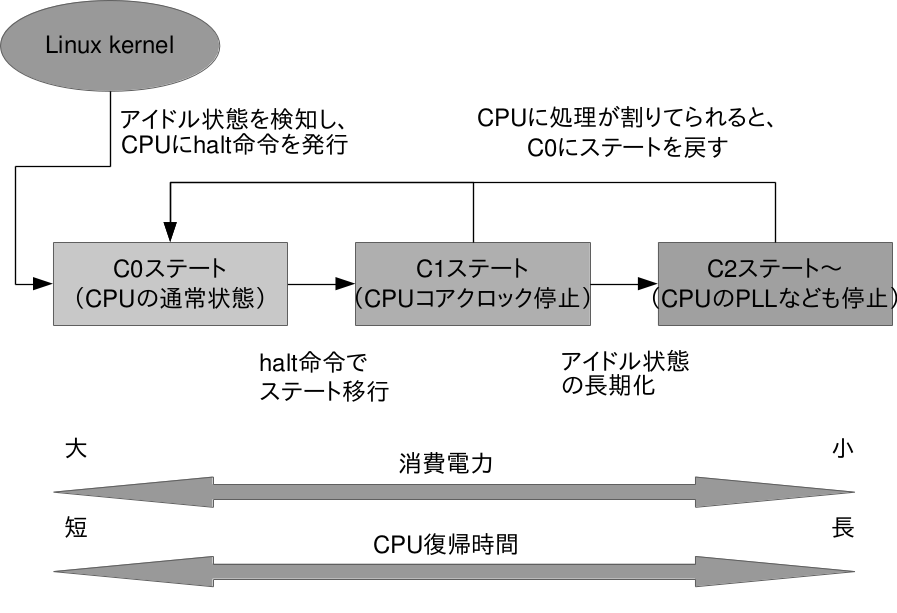
\includegraphics[width=0.5\hsize]{image201602/cpustate_mono.png}
\end{center}
\caption{CPU$B>uBVA+0\4J0W?^(B} 
\label{fig:cpustate}
\end{figure}

$B<B:]$N(BCPU$B$O(BC$B%9%F!<%H$@$1$G$O$J$/!"(BCPU$B$NEE05$d%/%m%C%/?t$J$I$b4XO"$7$F$-$^$9!#(B
Linux $B$N>l9g$O(BCPU$B<~GH?t%9%1!<%j%s%05!G=$r;H$&$3$H$G!"(BOS$B$,<+F0E*$K@)8f$G$-$k$h$&$K$J$C$F$$$^$9!#(B
$B$3$l$O(B Linux $B%+!<%M%k$N(B cpufreq $B$K$h$C$F<BAu$5$l$F$$$^$9!#(B
$B8=:_$N(B cpufreq $B$K@_Dj$5$l$F$$$kFbMF$r3NG'$9$k$K$O(B cpufrequtils $B%Q%C%1!<%8$GDs6!$5$l$F$$$k(B
cpufreq-info$B!J(B\fgref{fig:cpufreq-info}$B!K(B $B%3%^%s%I$r;H$$$^$9!#(B

\begin{figure}[htbp]
\begin{commandline}
$ cpufreq-info
cpufrequtils 008: cpufreq-info (C) Dominik Brodowski 2004-2009
Report errors and bugs to cpufreq@vger.kernel.org, please.
analyzing CPU 0:
  driver: intel_pstate
  CPUs which run at the same hardware frequency: 0
  CPUs which need to have their frequency coordinated by software: 0
  maximum transition latency: 0.97 ms.
  hardware limits: 800 MHz - 2.90 GHz
  available cpufreq governors: performance, powersave
  current policy: frequency should be within 800 MHz and 2.90 GHz.
                  The governor "powersave" may decide which speed to use
                  within this range.
  current CPU frequency is 1.90 GHz.
....
\end{commandline}

\caption{cpufreq-info $B<B9T7k2L(B}
\label{fig:cpufreq-info}
\end{figure}

$B$$$/$D$+9`L\$,$"$j$^$9$,!"=EMW$H$J$k$N$O(B $B!V(Bavailable cpufreq governors$B!W$H(B
$B!V(Bcurrent policy$B!W$G$9!#(B
available cpufreq governors $B$O(B CPU$B$ND4@02DG=$JB.EYD4@0L>!J%,%P%J!<!K$G$"$j!"(B
\tbref{tab:governors}$B$,MQ0U$5$l$F$$$^$9!#(B

\begin{table}[htb]
\begin{center}
\begin{tabular}{l|l}
$B%,%P%J!<(B & $BFbMF(B \\
ondemand &	CPU$BIi2Y$,Bg$-$$!"$^$?$O>.$5$$;~$K(BCPU$B%/%m%C%/$rBg$-$/$K@Z$jBX$($k(B \\
conservative &	CPU$BIi2Y$,Bg$-$$!"$^$?$O>.$5$$;~$K(BCPU$B%/%m%C%/$r=y!9$K@Z$jBX$($k(B \\
performance &	$B:GBg<~GH?t$G(BCPU$B$rF0:n$5$;$k(B \\
powersave &	$B:G>.<~GH?t$G(BCPU$B$rF0:n$5$;$k(B \\
userspace &	$B%f!<%6!<$,;XDj$7$?<~GH?t$G(BCPU$B$rF0:n$5$;$k(B \\
\end{tabular}
\caption{$B;XDj$G$-$k%,%P%J!<(B}
\label{tab:governors}
\end{center}
\end{table}

$B$3$l$i$O<B:]$K$O@_Dj$G$-$kCM%+!<%M%k$d4D6-$K$h$C$F0[$J$kE@$KCm0U$,I,MW$G$9!#(B
$B!V(Bcurrent policy$B!W$O8=:_@_Dj$5$l$F$$$k%,%P%J!<$,I=<($5$l$^$9!#(B

$B$3$N0J>e$+$i!">e5-$N7k2L$G$O(B

\begin{itemize}
\item CPU$B$,(B800MHz$B$+$i(B2.90GHz$B$^$G$r%5%]!<%H$7$F$$$k(B
\item powersave governor $B$GF0:n$7$F$$$k(B
\item $B:GBgCM$H:G>.CM$N%]%j%7!<@_Dj$K$h$j!"(B800MHz$B$+$i(B2.90GHz$B$N4V$GJQF0$5$;$F$$$k(B
\end{itemize}

$B$H$$$&$3$H$,$o$+$j$^$9!#(B

$B$3$l$i$r@_Dj$9$k$K$O(B sysfs $B7PM3$GA`:n$9$k$+!"(Bcpufrequtils $B$K4^$^$l$k(B
cpufreq-set $B%3%^%s%I$r;H$$$^$9!#(B

\begin{itemize}
\item $B%,%P%J!<$r@_Dj$9$k(B
  \begin{commandline}
   $ sudo cpufreq-set -c CPU$BHV9f(B -g $B%,%P%J!<L>(B
   $B$^$?$O(B
   $ sudo sh -c "echo $B%,%P%J!<L>(B > /sys/devices/system/cpu/cpuCPU$BHV9f(B/cpufreq/scaling_governor"
  \end{commandline}

\item $B:G>.%/%m%C%/$r@_Dj$9$k(B
  \begin{commandline}
   $ sudo cpufreq-set -c CPU$BHV9f(B -d $B%/%m%C%/CM(B
   $B$^$?$O(B
   $ sudo sh -c "echo $B%/%m%C%/CM(B > /sys/devices/system/cpu/cpuCPU$BHV9f(B/cpufreq/scaling_min_freq"
  \end{commandline}

\item $B:GBg%/%m%C%/$r@_Dj$9$k(B
  \begin{commandline}
   $ sudo cpufreq-set -c CPU$BHV9f(B -u $B%/%m%C%/CM(B
   $B$^$?$O(B
   $ sudo sh -c "echo $B%/%m%C%/CM(B > /sys/devices/system/cpu/cpuCPU$BHV9f(B/cpufreq/scaling_max_freq"
  \end{commandline}

\item $B8=:_$N%/%m%C%/$r@_Dj$9$k(B
  \begin{commandline}
   $ sudo cpufreq-set -c CPU$BHV9f(B -f $B%/%m%C%/CM(B
   $B$^$?$O(B
   $ sudo sh -c "echo $B%/%m%C%/CM(B > /sys/devices/system/cpu/cpuCPU$BHV9f(B/cpufreq/scaling_cur_freq"
  \end{commandline}

\end{itemize}

$B>e5-$N$h$&$K$7$F(BCPU$B%/%m%C%/$r@)8f$9$k$3$H$K$h$j!"4D6-$K$h$C$FL5BL$J$/(BCPU$B$rMxMQ$G$-$k$h$&$K$J$j$^$9!#(B
$B@_Dj$7$?CM$O:F5/F0$9$k$H>C$($k$N$G!"(B/etc/sysfs.conf $B$K@_Dj$7$F$*$/$+!"(Bcpufreq $B$r@_Dj$9$k%G!<%b%s(B cpufreqd
$B$r;H$&$H$h$$$G$7$g$&!#(B

\subsubsection{$BF0:n$7$F$$$k%G%P%$%9$N@_Dj(B}

$B;H$C$F$$$k8D!9$N%G%P%$%9$N@_Dj$b=EMW$H$J$j$^$9!#Nc$($PL5@~(BLAN$B$d(BBluetooth$B$r;H$o$J$$$N$KM-8z$K$7$F$$$k$H(B
$B$=$l$@$1$GEENO$r>CHq$7$F$7$^$$$^$9!#$h$C$F;HMQ$9$k4D6-$K1~$8$F$3$l$i$r@)8f$9$kI,MW$,=P$F$-$^$9!#(B

$B$3$3$G$O$h$/MxMQ$5$l$k%G%P%$%9$KBP$9$k@)8fJ}K!$K$D$$$F@bL@$7$^$9!#(B

\begin{itemize}

\item $B%i%C%W%H%C%W%b!<%I(B

Linux $B$N>l9g$O%+!<%M%k$N%b!<%I$H$7$F!"%i%C%W%H%C%W%b!<%I$,@_Dj$G$-$k$h$&$K$J$C$F$$$^$9!#(B
$B$3$l$O0J2<$N$h$&$K$7$F@_Dj$7$^$9!#(B

\begin{commandline}
$ sudo sh -c "echo 5 > /proc/sys/vm/laptop_mode"
\end{commandline}

$B$"$H(BNMI $B$N(Bwatchdog$B!J(Bnmi\_watchdog$B!K(B $B$bL58z2=$7$F$*$-$^$9!#$3$l$O$3$l$O%+!<%M%k%O%s%0%"%C%W$rDj4|E*$K%A%'%C%/$9$k5!9=(B
$B$r%3%s%H%m!<%k$9$k%U%i%0$G$9!#(B

\begin{commandline}
$ sudo sh -c "echo 0 > /proc/sys/kernel/nmi_watchdog"
\end{commandline}

\item USB

USB $B$O(B /sys/bus/usb/devices/ $B0J2<$KBP$7$F@_Dj$r9T$$$^$9!#(B
$BNc$($P!"(B/sys/bus/usb/devices/usb1 $B$KBP$7$F(B $BEE8;6!5k$r@Z$j$?$$>l9g$O(B /sys/bus/usb/devices/usb1/power/control
$B$r(Boff $B$K@_Dj$7$^$9!#<+F0E*$K%5%9%Z%s%I$5$;$?$$>l9g$K$O(B 
/sys/bus/usb/devices/usb1/power/autosuspend $B$KBP$7$F(B 1 $B$r@_Dj$7$^$9!#(B

\begin{commandline}
$ sudo sh -c "echo off > /sys/bus/usb/devices/usb1/power/control"
$ sudo sh -c "echo auto > /sys/bus/usb/devices/usb1/power/autosuspend"
\end{commandline}

$B@_Dj$r5/F0;~$KE,MQ$7$?$$>l9g$O!":F5/F0;~$K=i4|2=$5$l$F$7$^$&;v$H%G%P%$%9$N(BUSB$B0LCV$,JQ$o$k;v$,(B
$B$"$j$^$9$N$G!"(B udev $B$N(B rules $B%U%!%$%k$r;H$C$F@_Dj$9$k$N$,$h$$$G$7$g$&!#(B

\begin{commandline}
$B<B:]$O0l9T(B
$ cat /etc/udev/rules.d/70-my-usb-power.rules
ACTION=="add", SUBSYSTEM=="usb", ATTRS{idVendor}=="0x046d",
 ATTR{idProduct}=="0x08cb", TEST=="power/control", ATTR{power/control}="off"
\end{commandline}

$BCm0U$7$J$1$l$P$$$1$J$$E@$H$7$F$O(BUSB$B$r$J$s$G$b@_Dj$7$F$7$^$&$H%-!<%\!<%I$,F0:n$7$J$/$J$k2DG=@-$b$"$k$?$a!"(B
$B%Y%s%@!<(BID$B!"%G%P%$%9(BID$B$J$I$r3NG'$7$?>e$G@_Dj$7$^$7$g$&!#(B

\item $BL5@~(BLAN

$BL5@~(BLAN$B$O(B iw $B%Q%C%1!<%8$K4^$^$l$k(B iw $B%3%^%s%I$r;H$C$F@_Dj$7$^$9!#(B
$BL5@~(BLAN$B$,(Bwlan0$B$N>l9g$O(B $B0J2<$N$h$&$K@_Dj$9$k$3$H$K$h$C$F@)8f$G$-$^$9!#(B

\begin{commandline}
$ sudo iw dev wlan0 set power_save on
\end{commandline}

$B$3$l$b(Budev $B$N(B rules $B%U%!%$%k$r;H$C$F@_Dj$9$k$HNI$$$G$9!#(B

\begin{commandline}
$ cat /etc/udev/rules.d/70-my-wifi-power.rules
ACTION=="add", SUBSYSTEM=="net", KERNEL=="wlan*", RUN+="/usr/bin/iw dev %k set power_save on"
\end{commandline}

\item $B%5%&%s%I(B

$B%5%&%s%I$N>l9g$b(B sysfs $B7PM3$G@_Dj$7$^$9!#%I%i%$%P$K$h$C$F@_Dj=PMh$J$$>l9g$,$"$j$^$9$,!"(BINTEL $B$N%5%&%s%I(B
$B%3%s%H%m!<%i$N>l9g$O!"(Bpower\_save $B$,$"$k$N$G!"$3$l$r(B1$B$K@_Dj$9$k$3$H$K$h$C$F%Q%o!<%;!<%V%b!<%I$K@_Dj$G$-$^$9!#(B

\begin{commandline}
$ sudo sh -c "echo 1 > /sys/module/snd_hda_intel/parameters/power_save"
\end{commandline}

\item PCI/PCI-Express

PCI/PCI-Express $B$N>JEENO$K@_Dj$9$k$K$O(B power/control $B$r(B auto $B$K@_Dj$7$^$9!#(B
$B$3$N>l9g$b(B sysfs $B7PM3$G@_Dj$7$^$9!#(BPCI$B$b(BUSB$B$HF1MM$K@_Dj@h$,$I$N$h$&$J%G%P%$%9(B
$B$J$N$+3NG'$7$F$+$i@_Dj$9$k$h$&$K$7$^$7$g$&!#(B

\begin{commandline}
$ sudo sh -c "echo auto > /sys/bus/pci/devices/0000:00:00.0/power/control"
\end{commandline}

\end{itemize}

\subsubsection{$BF0:n$7$F$$$k%W%m%0%i%`$K$D$$$F(B}

$BF0:n$7$F$$$k%W%m%0%i%`$O(Btop$B%3%^%s%I$J$N$G$6$C$/$j$H$7$?(BCPU$B@jM-N($r3NG'$G$-$^$9$,!"<B:]$K(B
$B$I$l$0$i$$$NIQEY$G;H$o$l$F$F$$$k$N$+$o$+$j$^$;$s!#%"%$%I%k>uBV$G$"$k$K$b$+$+$o$i$:!"(BCPU$B3d$j9~$_$,B?$$(B
$B%W%m%0%i%`!&%W%m%;%9$,>JEENO$N8z2L$,F@$K$/$$$b$N$H$J$j$^$9$N$G!"$3$N$h$&$J%W%m%0%i%`!&%W%m%;%9$r(B
$BD4$Y$kI,MW$,$"$j$^$9!#$3$l$i$rD4$Y$k$K$O2<5-$G@bL@$9$k(B PowerTop $B$r;H$&$H$h$&$G$7$g$&!#(B

\subsection{$B>JEENO@_Dj$9$k$?$a$N%D!<%k(B}

$B@h$G$OD9!9$H=q$-$^$7$?$,!"CN<1$,$J$$%f!<%6$,>e5-$r0l$D$E$D$d$C$F$$$/$N$OHs>o$KBgJQ$G$9!#(B
Linux $B$G$O@lLg$NCN<1$,$J$/$H$b;H$C$F$$$k%^%7%s$r>JEENO>uBV$K@_Dj$G$-$k%D!<%k$,$$$/$D$+(B
$B=`Hw$5$l$F$$$^$9!#0J2<$G$O$=$l$i$N;H$$J}$K$D$$$F>R2p$7$^$9!#(B

\subsubsection{PowerTOP}

PowerTOP $B$O(BIntel$B$,3+H/$7$F$$$k%=%U%H%&%'%"$G!"%+!<%M%k!"%O!<%I%&%'%"!"%f!<%6%i%s%I$G@)8f2DG=$J>JEENO9`L\$r(B
$BM-8z$K$9$k%D!<%k$G$9!#%W%m%;%9$r4F;k$7$F!"(BCPU$BIi2Y$d%G%P%$%9%I%i%$%P$N;HMQ>u67$N%l%]!<%H$+$i%W%m%;%9$NA`:n(B
$B$r9T$&;v$,$G$-$^$9!#(B

\begin{enumerate}

\item $B%$%s%9%H!<%k(B

PowerTOP $B$O(BDebian $B$G$bDs6!$5$l$F$*$j!"(Bapt $B$G%$%s%9%H!<%k$G$-$^$9!#(B
\begin{commandline}
$ sudo apt-get install powertop
\end{commandline}

\item $B5/F0(B

$B5/F0$9$k$H(B\fgref{fig:powertop0}$B$N$h$&$J2hLL$,I=<($5$l$^$9!#(B
$B!V(BThe battery reports a discharge rate ...$B!W(B $B$K8=:_$N>CHqEENO$,(B
$BI=<($5$l!"8=:_F0:n$7$F$$$k%W%m%;%9$H;HMQ>u67$,$o$+$j$^$9!#(B
$BI.<T$N4D6-$G!"2?$b@_Dj$7$J$$>l9g$O(B 13W$B$N$h$&$G$9!#(B

\begin{figure}[H]
\begin{center}
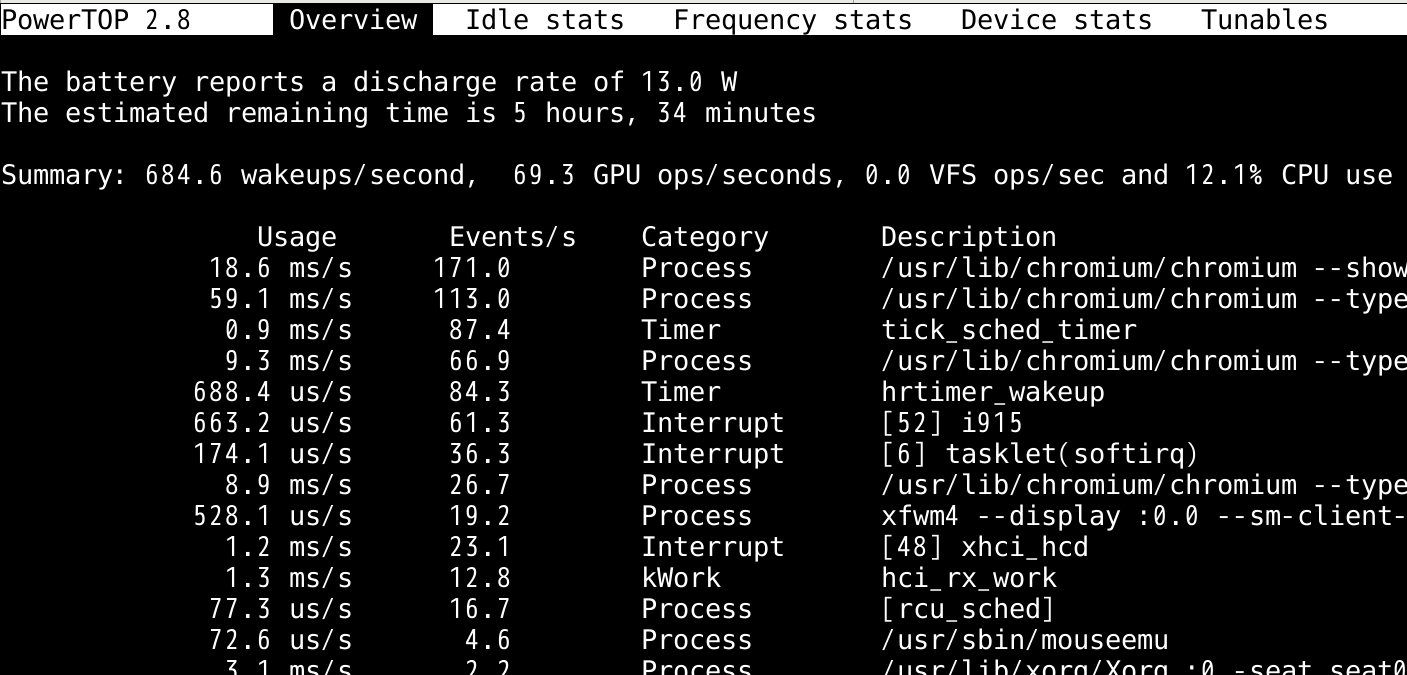
\includegraphics[width=0.5\hsize]{image201602/powertop_00.png}
\end{center}
\caption{PowerTOP$B5/F02hLL(B} 
\label{fig:powertop0}
\end{figure}

Tunables $B%?%V$rA*Br$9$k$HD4@02DG=$J%7%9%F%`$N@_Dj$,I=<($5$l$^$9(B(\fgref{fig:powertop1})$B!#(B
Bad$B$,>JEENO$KM-8z$J9`L\$K$b$+$+$o$i$:L58z$J@_Dj!"(B
Good $B$,4{$KM-8z$K$J$C$F$$$k@_Dj$H$J$C$F$$$^$9!#(B

\begin{figure}[H]
\begin{center}
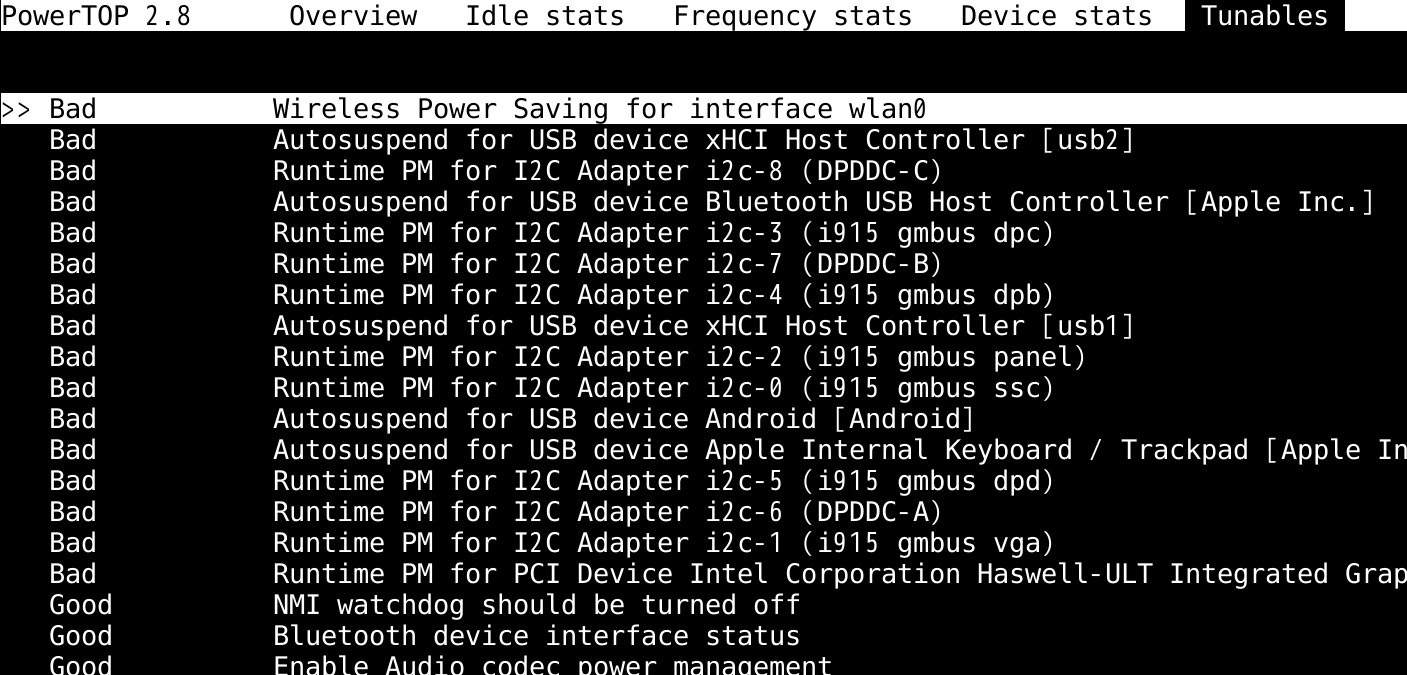
\includegraphics[width=0.5\hsize]{image201602/powertop_01.png}
\end{center}
\caption{Tunables$B2hLL(B} 
\label{fig:powertop1}
\end{figure}

$B$3$N>uBV$G$O$^$@%7%9%F%`$K:GE,2=$5$l$?@_Dj$K$J$C$F$$$J$$$?$a!"0lEY=*N;$7!"(B
$B%-%c%j%V%l!<%7%g%s$r9T$$$^$9!#(B

\item $B%-%c%j%V%l!<%7%g%s(B

$B@_Dj$9$k(BPC$B$N>uBV$r<hF@$9$k$?$a$K%-%c%j%V%l!<%7%g%s$r9T$$$^$9!#(B
$B<B9T$9$k$H%G%P%$%9$J$I$+$i;HMQ>u67$rFI$_<h$j!"%^%7%s$KBP$7$FE,@Z$J@_Dj$r(B
$B9T$$$^$9!#(B
$B%N!<%H(BPC$B$N>l9g$O$$$-$J$j%b%K%?!<$N%P%C%/%i%$%H$,>C$($k$N$GCm0U$7$^$7$g$&!#(B

\begin{commandline}
$ sudo powertop --calibrate
\end{commandline}

$B%-%c%j%V%l!<%7%g%s$,=*$o$k$H!"(B\texttt{/var/cache/powertop/saved\_parameters.powertop}
$B0J2<$K%G!<%?$,J]B8$5$l$^$9!#<!2s$N(BPowerTOP$B5/F0;~$+$i$O%-%c%j%V%l!<%7%g%s%G!<%?$r85$K(B
$B>JEENO$K$5$l$?4D6-$G5/F0$7$^$9!#(B

\item $B%-%c%j%V%l!<%7%g%s8e(B

$B%-%c%j%V%l!<%7%g%s8e$K5/F0$9$k$H!"(B
$B!V(BThe battery reports a discharge rate ...$B!W(B $B$N9`L\$KI=<($5$l$k>CHqEENOCM$,JQ$o$j!"%7%9%F%`(B
$BA4BN$G>JEENO$G2TF/$7$F$$$k$3$H$,3NG'$G$-$k$G$7$g$&!#(B

\item PowerTOP $B$N5/F0;~M-8z2=(B

PowerTOP $B$O5/F0$9$k$HJ]B8$5$l$F$$$k@_Dj$r85$K>JEENO>uBV$K$7$F$/$l$^$9$,!"(BPC$B$rN)$A>e$2$k$?$S$K(B
PowerTOP$B<+BN$rN)$A>e$2$kI,MW$,$"$j$^$9!#(B

$B5/F0;~$K<+F0E*$K(BPowerTOP $B$rN)$A>e$2$k$h$&$K$9$k$K$O!"0J2<$N$h$&$K(B systemd $B$N(B $B%f%K%C%H%U%!%$%k(B
$B$rMQ0U$7!"M-8z$K$7$F$*$-$^$9!#(B

\begin{commandline}
$ cat /etc/systemd/system/powertop.service

[Unit]
Description=PowerTOP

[Service]
Type=oneshot
ExecStart=/usr/bin/powertop
Environment="TERM=xterm"

[Install]
WantedBy=multi-user.target
\end{commandline}

\begin{commandline}
$ sudo systemctl enable powertop
\end{commandline}

\end{enumerate}

\subsubsection{TLP $B$r;H$C$?@_Dj(B}

PowerTOP $B$NB>$K(BTLP$B$H$$$&%D!<%k$b$"$j$^$9!#$3$l$O(B PowerTOP$B$N$h$&$K>\:Y$J%l%]!<%H$O(B
$B=P$7$F$/$l$^$;$s$,!"(BAC$B@\B3;~$J$I$N>u67$K1~$8$?%9%/%j%W%H$,=`Hw$5$l$F$*$j!"%$%s%9%H!<%k(B
$B$9$k$@$1$G$"$kDxEY>JEENO@_Dj$r9T$C$F$/$l$kJXMx$J%D!<%k$G$9!#(B
$B$b$A$m$s!"(BDebian $B$G$O%Q%C%1!<%82=$5$l$F$*$j!"(Bapt $B$G%$%s%9%H!<%k$G$-$^$9!#(B

\begin{commandline}
$ sudo apt-get install tlp
\end{commandline}

$BL5@~(BLAN$B$N@_DjEy$K(B NetworkManager $B$r;H$C$F$$$k$J$i(B tlp-rdw $B%Q%C%1!<%8$b%$%s%9%H!<%k$7$F$*$/$H(B
$BL5@~(BLAN$B!"(BBluetooth$B4XO"$N@_Dj$b9T$C$F$/$l$^$9!#(B
$B%G%U%)%k%H$N@_Dj$O(B /etc/default/tlp $B$K$"$j!"$3$N%U%!%$%k$rJQ99$7$F4D6-$K9g$o$;$?>JEENO@_Dj$r(B
$B9T$$$^$9!J(B\fgref{fig:TLP}$B!K!#@_Dj$O$h$/;H$o$l$k9`L\$7$+$J$/!";H$C$F$$$k4D6-$N@_Dj$,$J$$>l9g$b$"$j$^$9!#$3$N$h$&$J>l9g$O(B
T$B<+J,$G@_Dj$rDI2C$9$k$+!"@h$K@bL@$7$?$h$&$K(Bsysfs / procfs $B7PM3(B
$B$N@_Dj$rJLES9T$&I,MW$,$"$j$^$9!#(B


\begin{figure}[H]
\begin{center}
\begin{commandline}
# Set to 0 to disable, 1 to enable TLP.
TLP_ENABLE=1

# Operation mode when no power supply can be detected: AC, BAT
# Concerns some desktop and embedded hardware only.
TLP_DEFAULT_MODE=AC

# Seconds laptop mode has to wait after the disk goes idle before doing a sync.
# Non-zero value enables, zero disables laptop mode.
DISK_IDLE_SECS_ON_AC=0
DISK_IDLE_SECS_ON_BAT=2

# Dirty page values (timeouts in secs).
MAX_LOST_WORK_SECS_ON_AC=15
MAX_LOST_WORK_SECS_ON_BAT=60
...
\end{commandline}
\end{center}
\caption{/etc/default/tlp $BNc(B} 
\label{fig:TLP}
\end{figure}

TLP $B$O(B systemd $B$d$=$NB>(Binit$BMQ$N5/F0%U%!%$%k$,MQ0U$5$l$F$$$k$N$G(BPC$B5/F0;~$K@_Dj$,H?1G$5$l$k$N$b(B
$BNI$$E@$G$9!#(B

\subsubsection{$B>JEENO@_Dj8e(B}
\fgref{fig:powertop2}$B$,>JEENO@_Dj$7$?8e$K(B PowerTOP $B$G>CHqEENO$r3NG'$7$?FbMF$G$9!#(B
$B>CHqEENO$,(B13W $B$+$i(B 11W $B$K2<$,$C$F$$$k$3$H$,$o$+$j$^$9!#$^$?(BPC$B2TF/;~4V$b(B5$B;~4VH>$+$i(B6$B;~4V(B50$BJ,$K(B
$B?-$S$F$$$k$3$H$,$o$+$j$^$9!#(B

\begin{figure}[H]
\begin{center}
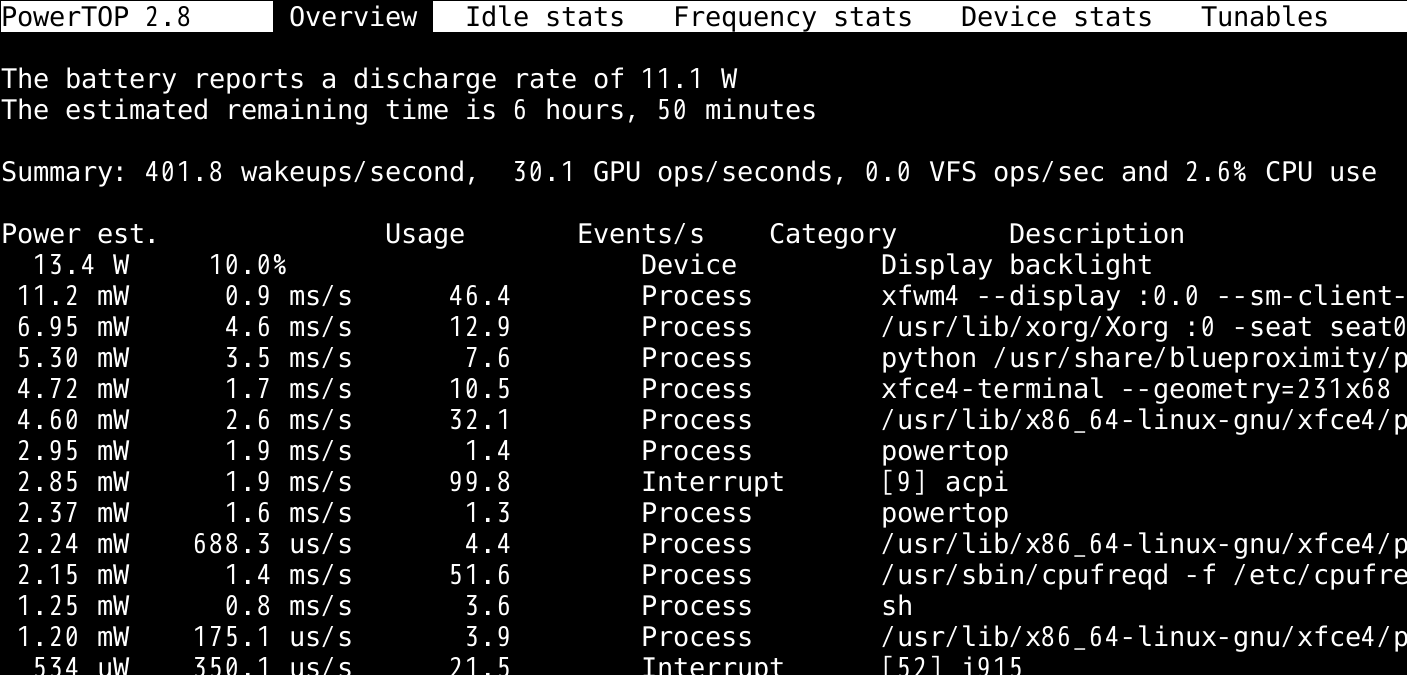
\includegraphics[width=0.5\hsize]{image201602/powertop_02.png}
\end{center}
\caption{$B>JEENO@_Dj8e(B} 
\label{fig:powertop2}
\end{figure}

\subsection{$B$^$H$a(B}

Debian $B$G$N>JEENO@_Dj$K$D$$$F@bL@$7$^$7$?!#(B
$B8=:_$N>uBV$r$H$j$"$($:3NG'$9$k$K$O(B cpufreq-info $B$r;H$$!"%+!<%M%k$N@_Dj$d%I%i%$%P$N@_Dj$O(B
sysfs $B$d(B proc fs $B7PM3$G@_Dj$7$^$9!#%W%m%0%i%`$d%W%m%;%9$N>\:Y$J>uBV$N3NG'$9$k$K$O(B PowerTOP
$B$r;H$$$^$9!#>JEENO@_Dj$G$-$k9`L\$b$o$+$j!"%f!<%6%$%s%?!<%U%'%$%9$+$i3F<o@_Dj$,$G$-$k$h$&$K$J$C$F$$$^$9!#(B
$B$^$?:FN)$A>e$2$9$k$H>JEENO@_Dj$r:F@_Dj$9$kI,MW$,$"$j$^$9$N$G!"(Bsysytem$BMQ$N(Bservice
$B%U%!%$%k$rJLESMQ0U$9$k$J$I$NBP:v$,I,MW$G$9!#(B
$B:Y$+$$@_Dj$r9T$o$J$/$F$b!"$H$j$"$($:>JEENO@_Dj$r9T$$$?$$>l9g$O(BTLP$B$r;H$&$N$,$h$$$G$7$g$&!#$?$@A4$F$N(B
PC$B$r%5%]!<%H$7$F$$$k$o$1$G$O$"$j$^$;$s$N$G!"4D6-$K9g$o$;$F%W%m%0%i%`$r=$@5$9$k$J$j$NBP1~$,I,MW$H$J$j$^$9!#(B

\dancersection{LibreOffice$B$N:G6a$NF08~$H(BDebian$B$G$N(BLibreOffice$B%Q%C%1!<%8$K$D$$$F(B}{$B1](B $B??<#(B}

\subsection{2015$BG/$N(BLibreOffice$B$r?6$jJV$C$F(B}
\begin{itemize}
\item %
LibreOffice Online(LOOL)$B$N3+H/$,K\3J3+;O(B
\item %
LibreOffice Viewer$B%j%j!<%9(B
\item %
$BJT=85!G=$O<B83E*$JCJ3,(B
\item %
$B3+H/(B/$B%j%j!<%9$b=gD4$K(B
\item %
$B5!G=LL0J30$G$b!"(BUX$B$N2~A1$K<h$jAH$_(B
\item %
$BAj8_1?MQ@-!J%U%#%k%?!K$N2~A1(B
\item %
2015$BG/(B9$B7n$K$O#5<~G/!*(B
\end{itemize}

\subsection{LibreOffice Online}
\begin{itemize}
\item %
$B$^$@$^$@3+H/Cf(B
\item %
UI$B$,(BHTML5$B!"%V%i%&%6$GJT=8$9$k(B
\item %
$BJ#?t%f!<%6!<$NF1;~JT=8(B
\item %
$B%5!<%P!<%W%m%0%i%`$H$7$FDs6!(B
\item %
$BC/$G$b%5!<%P!<$r$?$F$i$l$k(B
\item %
$B%[%9%F%#%s%0%5!<%S%9$b=P$F$/$k$N$G$O(B
\item ownCloud$B$NJT=82hLL$G(BLOOL$B$r;H$&%G%b(B
\url{https://www.youtube.com/watch?v=jPGBRu085Dw}
\end{itemize}

\subsection{$B%W%m%8%'%/%H$N>u67(B}
\begin{itemize}
\item %
Advisory Board$B!J8=:_(Bweb$B$G$O(B17$B!K(B
\item %
CIB, $B%_%e%s%X%s;T(B,Rusbitech$B$,$3$N(B1$BG/$G;22C(B
\item %
$B%"%/%F%#%V$J%3%_%C%?!<$OKh7n(B100$B?MDxEY(B
\item %
TDF$B$N%9%?%C%U$O(B6$BL>!J%a%s%P!<(B211$BL>!K(B
\item %
TDF$B%a%s%P!<0J30$G$b%"%/%F%#%V$J?M$OB?$$(B
\item %
$B%h!<%m%C%Q$G$O9T@/Cf?4$KF3F~$,?J9TCf(B
\item %
$B%$%?%j%"9qKI>J(B15$BK|Bf(B
\item %
$B%U%i%s%9FbL3>J(B24$BK|Bf!J$3$l$O0JA0$+$i!K(B
\item %
$B%$%.%j%9@/I\$b(BODF $BI8=`!"(BCollabora$B$H$b7@Ls$7(BLibreOffice$BF3F~$X(B
\item %
$BBfOQ$b(BODF$B?d?J!"<+<#BN$G(BLibreOffice$BF3F~(B
\end{itemize}

\subsection{$B:#G/$NF|K\$G$N3hF0(B}
\begin{itemize}
\item %
$BK]Lu(B
\item %
UI$B$NK]LuN($O9b$$(B,Help$B$O$^$9$^$9DI$$$D$$$F$J$$(B\\
$B!JK]LuN($O9b$/$F$b8mLu$r8+$D$1$F=$@5$7$-$l$F$J$$!"$H$N%D%C%3%_$"$j!K(B
\item %
$B1Q8l$N(BHelp$B$b<BAu$KDI$$$D$$$F$J$$%1!<%9$b(B
\item %
$B%I%-%e%a%s%H7OK]Lu$O%"%J%&%s%9$/$i$$(B
\item %
$BK]Lu::FI%9%W%j%s%H$r3+:E(B($B::FI$,N/$^$C$F$-$F$$$?(B+$B%k!<%k$N5DO@!K(B
\item %
$BIJ<AJ]>Z(B
\item %
HackFest (Bug$B%O%s%F%#%s%0(B)7$B2s(B
\item %
$B%/%i%C%7%e%P%0$J$I$$$/$D$+H/8+(B/$B%l%]!<%H(B
\end{itemize}

\subsection{$B:#G/$NF|K\$G$N3hF0(B2}
\begin{itemize}
%\item %
%$B%$%Y%s%H(B
\item %
$BF|K\8l%3%_%e%K%F%#$N%$%Y%s%H(B+$B%V!<%9=PE8$J$I(B46$B2s(B
\item %
HackFest $B$rA}$d$7$?!J(B10$B2s!K!"MhG/$b=EE@E*$K(B
\item %
QA$B$J$I=8$^$C$F$d$k$3$H$G:n6H$,$d$j$d$9$+$C$?(B
\item %
$B$^$@$^$@;22C<T$O>/$J$$(B
\item %
$B3+H/8~$1$b(B1$B2s!"(BLibreOffice$B$N%S%k%I%M%?$GD)@o(B
\item %
$B4X@>(BLibreOffice HackFest 2015-08-22($B3+H/(B)
\item %
LibreOffice Hackfest ($BK]Lu::FI%9%W%j%s%H(B) 2015-07-26 in $BEl5~(B
\end{itemize}

\subsection{LibreOffice Conference 2015}
\begin{itemize}
\item %
$B3+:ECO!'%G%s%^!<%/!&%*!<%U%9(B
\item %
$BF|;~!'(B2015/9/23($B?e(B)-25($B6b(B)
\item %
$BLs(B80$B$N%;%C%7%g%s(B
\item %
$B;22C<T!'Ls(B150$BL>(B
\item %
$BNcG/$h$jB?$a!"%"%8%"@*$bA}$($?(B
\item %
$BF|K\$+$i$O(B3$BL>(B
\item %
$B>.3^86$5$s!";3K\$5$s!"1](B
\item %
NLP$B%o!<%/%7%g%C%W(B
\item %
ITPro$B$G$N%+%s%U%!%l%s%9%l%]!<%H(B\url{http://itpro.nikkeibp.co.jp/atcl/column/15/102800252/}
\end{itemize}

%$B$H$j$H$a$J$$ItJ,$J$N$G!">JN,(B
%\subsection{$B3F8@8l$N%3%_%e%K%F%#(B}
%\item %
%LibreItalia$B!JHs1DMxCDBN!K(B
%\item %
%$B650i8~$1$b3hH/!'65;U8~$1!"J]8n<T8~$1!";R6!8~$1(B
%\item %
%$B%Y%H%J%`%3%_%e%K%F%#(B
%\item %
%$BJ*M}E*$J5wN%$,N%$l$F$$$k!#%k!<%k:n$j$r$7$?(B
%\item %
%MSO$B$O1Q8l(BUI$B$7$+$J$$$,!"2?$r$I$3$^$GK]Lu$9$k$+!)(B
%\item %
%LibreOffice$B$@$1$r$d$C$F$$$k?M$O$[$\$$$J$$(B
%\item %
%$BJ#?t$N%3%_%e%K%F%#$r$+$1$b$A(B
%\item %

%$B3+:E8e$J$N$G%l%]!<%H%Y!<%9$N;qNA$G99?7(B
\subsection{LibreOffice mini Conference 2016 in Japan$B$r3+:E$7$^$7$?(B}
\begin{itemize}
\item %
$BF|;~!'(B2016/1/9($BEZ(B) 13:00-18:00
\item %
$B>l=j!'(BGMO Yours!$B!J%0%i%s%U%m%s%HBg:e!K(B
\item %
$B;22C<T!'(B48$BL>(B
\item %
ITPro$B$G$N%+%s%U%!%l%s%9%l%]!<%H(B\url{http://itpro.nikkeibp.co.jp/atcl/column/14/090100053/013100122/}
\end{itemize}

\subsection{Debian$B$G$N(BLibreOffice$B%Q%C%1!<%8(B}

TDF$B$GDs6!$5$l$F$$$k%=!<%9%3!<%I$r(BTDF$BHG!"(B
Debian$B$G(Bapt-get source$B$G<hF@$G$-$k%=!<%9%3!<%I$r(BDebian$BHG$H!"$3$N;qNA$G$O8F$V$3$H$K$7$^$9(B
\subsection{TDF$BHG$N%=!<%9$rMn$H$7$F$_$k(B}
\begin{commandline}
$ tar -Jxvf libreoffice-4.3.3.2.tar.xz 
$ du -h libreoffice-4.3.3.2
931M libreoffice-4.3.3.2
\end{commandline}
Debian$BHG$N%=!<%9$r<hF@$9$k(B
Debian$B%Q%C%1!<%8$N%=!<%9$r<hF@$9$k!J4D6-!'0BDjHG(Bjessie$B!K(B
\begin{commandline}
$ sudo aptitude install dpkg-dev
$ apt-get source libreoffice

$ ls -lh
drwxr-xr-x 153 eno eno  48K 12$B7n(B 26 21:06 libreoffice-4.3.3
-rw-r--r--   1 eno eno 2.1M  9$B7n(B  5 03:25 libreoffice_4.3.3-2+deb8u2.debian.tar.xz
-rw-r--r--   1 eno eno  26K  9$B7n(B  5 03:25 libreoffice_4.3.3-2+deb8u2.dsc
-rw-r--r--   1 eno eno 308M  4$B7n(B  9  2015 libreoffice_4.3.3.orig-external.tar.xz
-rw-r--r--   1 eno eno 1.4M  4$B7n(B  9  2015 libreoffice_4.3.3.orig-helpcontent2.tar.xz
-rw-r--r--   1 eno eno 122M  4$B7n(B  9  2015 libreoffice_4.3.3.orig-translations.tar.xz
-rw-r--r--   1 eno eno 143M  4$B7n(B  9  2015 libreoffice_4.3.3.orig.tar.xz
\end{commandline}
\subsection{external$B$O!"B>$N(BOSS$B$N$3$H(B}
\begin{itemize}
\item %
Debian$BHG$O!"B>$N(BOSS$BK\BN$N%=!<%9%3!<%I$r4^$`(B
$B!I(Bexternal/tarballs/$B!I0J2<(B
Python3, hsqldb, poppler, $B3F<o%U%)%s%H$J$IBgNL$K(B
\item %
TDF$BHG$O!"B>$N(BOSS$B$X$N%Q%C%A$N$_(B
$B=i$a$F(Bmake$B$9$k;~$KB>$N(BOSS$B$NK\BN$O%@%&%s%m!<%I(B
$B$J$N$G(B1$B2sL\$N%S%k%I$O7k9=;~4V$,$+$+$k(B
\end{itemize}
\subsection{$B%U%!%$%k0lMw$N(Bdiff$B!J(BDebian$BHG$K$7$+$J$$$b$N!K(B}
\begin{commandline}
/.pc/$B!!0J2<(B745$B!!(B.pc/$B0J2<$O(Bquilt$B$N(BDebian$B8~$1=$@55-O?(B 
/bridges/$B!!0J2<(B7
/translations/$B0J2<!!(BTDF$BHG$OK]Lu!"%X%k%W$OJL$K$J$C$F$$$k(B
/helpcontent2/$B0J2<(B
/debian/$B0J2<(B131$B!!(Bdebian/$B0J2<$O(Bdebian$BFH<+%Q%C%A(B
/external/tarballs/$B0J2<(B109
/solenv/gbuild/platform/LINUX_AARCH64_GCC.mk$B!!$=$l0J30$K!"(B3$B%U%!%$%k$[$IDI2C$5$l$F$$$k(B...
/writerfilter/qa/cppunittests/rtftok/data/pass/sf_2063317381c4a46d642c79a4b1817dc0-101375-minimized.rtf
/writerfilter/qa/cppunittests/rtftok/data/pass/sf_2063317381c4a46d642c79a4b1817dc0-108116-minimized.rtf
\subsection{libreoffice-4.3.3$B$N%G%#%l%/%H%j9=@.(B}
$ du -h libreoffice-4.3.3/
...
2.7G libreoffice-4.3.3/
$BFb!"(Btranslations/$B0J2<$,(B1.5G$B$HBg$-$J3d9g$r@j$a$k(B

$ cd libreoffice-4.3.3/
$ du -h debian/
4.0K	debian/pyuno-for-2.7
44K	debian/scripts
488K	debian/patches
12K	debian/source
8.0K	debian/branding
12K	debian/tests/patches
24K	debian/tests
2.9M	debian/templates
8.0K	debian/upstream
5.0M	debian/
\end{commandline}
\subsection{libreoffice-4.3.3/debian/patches/$B$K4^$^$l$k%U%!%$%k(B}
\begin{itemize}
\item %
46$B$N%Q%C%A%U%!%$%k(B
\item %
$B%;%-%e%j%F%#(BFIX$B$N%Q%C%A$O(B6$B$D!"%;%-%e%j%F%#(BFIX$B$OBP1~$G$-$F$$$k$h$&(B
\footnote{\url{https://www.libreoffice.org/about-us/security/advisories/}}
\item %
libreoffice$B$N(Bmaster$B$+$i<h$j9~$_(B6$B$DDxEY!"$=$l0J30$N(Bmaster$B$+$i<h$j9~$_$b$"$k(B
\item %
$B$=$NB>!"(BDebian$B$N@_Dj$d%S%k%I<~$j$N%Q%C%A$G(B
$B!J$6$C$H$_$?46$8$G$O!K(BDebian$BFH<+$N5!G=$O$J$5$=$&(B
\end{itemize}

%Debian $B$G$NJQ99MzNr(B
%\begin{commandline}
%backport-rtf-fixes.diff (CVE-2014-9093)
%Bug 86449 - Crash importing malformed .rtf
%\end{commandline}

\subsection{Debian$B$N(BLibreOffice$B%P!<%8%g%s(B(2015$BG/(B12$B7n;~E@(B)}
\begin{itemize}
\item %
experimental: $B8=:_(B 1:5.1.0~rc1-1
LibreOffice$B$N3+H/HG!#(B5.1$B7O(BAlpha $B"*(B Beta $B"*%j%j!<%98uJd(B(RC)
\item %
sid$B!J(Bstretch$B$bF1$8!K(B: $B8=:_(B 1:5.0.4~rc2-2
LibreOffice$B$N:G?7HG(B(fresh)$B$N%j%j!<%98uJd$H%j%j!<%9HG(B
\item %
jessie(Stable) : $B8=:_(B 1:4.3.3-2+deb8u2
2$B2s%"%C%W%G!<%H(B (2015/3/26: CVE-2015-1774, 2015/8/28 : CVE-2014-4551,VE-2015-5213,CVE-2015-5212,CVE-2015-5214)
sid$B;~Be$K(B1$B2s%;%-%e%j%F%#(BFIX (2014/11/27 : CVE-2014-9093)
\item %
jessie-backports: $B8=:_(B 1:5.0.4~rc2-2
LibreOffice$B$N:G?7HG(B(fresh)$B$H$=$N%j%j!<%98uJd(B
$B0BDjHG(B(jessie)$B$G$b(BLibreOffice$B$N:G?7HG$,MxMQ$G$-$k(B
\end{itemize}
\begin{center}
Enjoy Debian and LibreOffice Life!
\end{center}

\subsection{$BCx<T>R2p(B}
\begin{itemize}
\item %
$B1]??<#!J$($N$-$7$s$8!K(B
\item %
LibreOffice$BF|K\8l%A!<%`%a%s%P!<(B(2011-$B8=:_(B)
$B<g$K%$%Y%s%HC4Ev!"(B2015$BG/$O(BLibreOffice$B%3%_%e%K%F%#%$%Y%s%H(B34$B2s$/$i$$3+:E(B/$B;22C(B
%\item %
%$B:#F|$_$?$$$J$N$O%+%&%s%H30$G$9(B
\item %
The Document Foundation$B%a%s%P!<(B(2014/4-$B8=:_(B)
\item %
$B%U%j!<$G(BLibreOffice$B$N%3%s%5%k(B/$B%5%]!<%H(B/$B%H%l!<%K%s%0(B
\item %
$B%"%$%/%i%U%H3t<02q<R$HAH$s$G(BLibreOffice$B%5%]!<%H%S%8%M%9(B
$B!J(BCollabora$B$N%5%]!<%H$N%j%;!<%k$H(BL1/L2$B%5%]!<%H!K$r3+;O(B
\end{itemize}

%201512
\dancersection{Debian $B%b%P%$%k(B wifi $B%k!<%?2=(B}{$BLnEg(B $B5.1Q(B}

\subsection{$B$O$8$a$K(B}

 $B:G6a$N%b%P%$%k%k!<%?$O!"(B7GBytes/$B7n!"(B300MBytes/$BF|$J$I$N!"0lDj$NDL?.NL$rD6$($k$H$?$A$^$ADL?.@)8B$,$+$+$C$F$7$^$$!"$H$F$b<BMQ$K$J$i$J$$$0$i$$$KDL?.BS0h$r9J$i$l$F$7$^$$$^$9!#(B
  
$B!!$?$^$?$^!"<j85$KDL?.@)8B$,Hs>o$K$f$k$$!J$H$$$&$+5$$K$J$i$J$$!K(BFOMA$B$N%b%G%`$,$"$j$^$7$?$N$G!"$3$A$i$H(BDebian$B$r;H$C$F%b%P%$%k%k!<%?$,:n$l$J$$$+$r;n$7$F$_$^$7$?!#$^$?!"(BLinux$B$GL5@~(BAP$B$r:n$k;~$N;EAH$_$K$D$$$F$b$A$g$C$HD4$Y$F$_$^$7$?!#(B
 


\subsection{$BMQ0U$9$k$b$N(B}

  $BMQ0U$9$k$b$N$O<!$N$H$*$j!#(B

  \begin{itemize}
  \item Debian$B$NF0$/%b%P%$%k(BPC
  \item DoCoMo$B<R(B L-05A ($B%b%G%`!#%G!<%?Dj3[@)$N7@Ls$G$"$k$3$H!#(B)
  \item BUFFALO WLI-UC-GNM2 ($BHw9M!'(BRalink$B@=(B Ralink RT3070$BEk:\!#(B900$B1_(B/1$B8D$0$i$$$N>.7?(BUSB$BL5@~(BLAN$B%"%@%W%?!K(B
  \end{itemize}    



\subsection{bridge$B$r:n$k(B}

  \begin{description}
    \item [Step 1-1] apt install bridge-utils
    \item [Step 1-2] vi /etc/network/interface$B$7$F0J2<$rDI5-(B
  \end{description}      
 /etc/network/interface$B$NDI5-ItJ,!'(B
\begin{commandline}
auto br0
iface br0 inet static
        address 192.168.0.1
        netmask 255.255.255.0
        bridge_ports none
        bridge_stp off
        bridge_fd 0
        bridge_maxwait 0
\end{commandline}

  \begin{description}
    \item [Step 1-3] ifup br0
    \item [Step 1-4] vi /etc/sysctl.d/bridge-filter-workaround.conf
  \end{description}      
/etc/sysctl.d/bridge-filter-workaround.conf$BCf?H!'(B
\begin{commandline}
net.bridge.bridge-nf-call-ip6tables = 0
net.bridge.bridge-nf-call-iptables = 0
net.bridge.bridge-nf-call-arptables = 0
\end{commandline}

  \begin{description}
    \item [Step 1-5] vi /etc/sysctl.d/forward-yes.conf
  \end{description}      
 /etc/sysctl.d/forward-yes.conf$BCf?H!'(B
\begin{commandline}
net.ipv4.ip_forward=1
\end{commandline}

  \begin{description}
  \item [Step 1-6] sysctl -p /etc/sysctl.d/bridge-filter-workaround.conf
  \item [Step 1-7] sysctl -p /etc/sysctl.d/forward-yes.conf
$B!!(B\end{description}

\begin{figure}[htbp]
\includegraphics[width=0.5\hsize]{image201512/bridge.eps}
\caption{bridge$B$N@_Dj$N>u67(B}
\end{figure}
  
\subsection{L-05A$BB&@_Dj(B}

  \begin{description}
    \item [Step 2-1] apt install ppp
    \item [Step 2-2] vi /etc/ppp/peers/l-05a
  \end{description}      


 /etc/ppp/peers/l-05a$B$NCf?H!'(B
\begin{commandline}
hide-password 
noauth 
connect "/usr/sbin/chat -v -f /etc/chatscripts/l-05a"
debug 
/dev/ttyACM0
115200
defaultroute
noipdefault 
user ""
remotename l-05a
ipparam l-05a
persist 
usepeerdns 
idle 300
\end{commandline}
  
  \begin{description}
    \item [Step 2-3] vi /etc/chatscripts/l-05a
  \end{description}      
 /etc/chatscripts/l-05a$B$NCf?H!'(B
\begin{commandline}
ABORT BUSY ABORT 'NO CARRIER' ABORT VOICE 
ABORT 'NO DIALTONE' ABORT 'NO DIAL TONE' 
ABORT 'NO ANSWER' ABORT DELAYED
'' ATZ
OK-AT-OK "ATDT*99***5#"
CONNECT \d\c
\end{commandline}

  \begin{description}
    \item [Step 2-4] chown root:dip /etc/ppp/peers/l-05a /etc/chatscripts/l-05a
    \item [Step 2-5] chmod 640 /etc/ppp/peers/l-05a /etc/chatscripts/l-05a
    \item [Step 2-6] vi /etc/ppp/ip-up.d/bridge-up
  \end{description}      
 /etc/ppp/ip-up.d/bridge-up$B$NCf?H!'(B
\begin{commandline}
#!/bin/sh
iptables -t nat -A POSTROUTING -o $PPP_IFACE \
-j MASQUERADE
iptables -A FORWARD -i br0 -o $PPP_IFACE -j ACCEPT
iptables -A FORWARD -o br0 -i $PPP_IFACE -j ACCEPT
\end{commandline}

  \begin{description}
    \item [Step 2-7] vi /etc/ppp/ip-down.d/bridge-down
  \end{description}      
 /etc/ppp/ip-down.d/bridge-down$B$NCf?H!'(B
\begin{commandline}
#!/bin/sh
PATH=/bin:/usr/bin:/sbin:/usr/sbin
iptables -t nat -D POSTROUTING -o $PPP_IFACE \
-j MASQUERADE
iptables -D FORWARD -i br0 -o $PPP_IFACE -j ACCEPT
iptables -D FORWARD -o br0 -i $PPP_IFACE -j ACCEPT
\end{commandline}

  \begin{description}
    \item [Step 2-8] chown 755 /etc/ppp/ip-up.d/bridge-up /etc/ppp/ip-up.d/bridge-down
    \item [Step 2-9] pon l-05a
  \end{description}      
 $B$3$l$G!"(BL-05a$B$O%0%m!<%P%k$K@\B3$5$l$k$h$&$K$J$j$^$9!#(B

\begin{figure}[htbp]
\includegraphics[width=0.5\hsize]{image201512/pppd.eps}
\caption{ppp$B$N@_Dj$N>u67(B}
\end{figure}

\subsection{$BJdB-!'(BL-05A$BB&%H%i%V%k%7%e!<%H(B}

 $B$D$J$,$i$J$$;~$O<!$N$H$*$j$G$9!#(B

 \begin{itemize}
 \item tail -f /var/log/debug /var/log/messages$B$K>\:Y$J%m%0$,=P$^$9!#$3$A$i$r8+$k$H2r7h$N$?$a$N%R%s%H$,8+$D$+$j$^$9!#(B
 \item pon l-05a$B$r$7$?8e!"(BttyACM0$B$,8+$D$+$i$J$$$H$$$&%(%i!<$,=P$k$3$H$,$"$j$^$9!#$3$N>l9g$O!"<!$N<jB3$-$r<h$k$H<#$j$^$9!#(B\\
 modprobe -r uas;modprobe uas;eject /dev/sr0
 \end{itemize} 



\subsection{hostapd$B$N@_Dj(B}

  $B$$$h$$$hL5@~(BAP$B$rN)$F$^$9!#(B

  \begin{description}
  \item [Step 3-1] apt install hostapd firmware-ralink
  \item [Step 3-2] $B$3$3$G!"(BWLI-UC-GNM2$B$r(BPC$B$K:9$79~$`!#(B
  \item [Step 3-3] lsmod$B$7$F0J2<$N%b%8%e!<%k$,%m!<%I$5$l$?$3$H$r3NG'!#(B
  \end{description}      
 lsmod$B$N7k2LH4?h(B
\begin{commandline}
rt2800usb              28672  0
rt2x00usb              24576  1 rt2800usb
rt2800lib              90112  1 rt2800usb
rt2x00lib              53248  3 rt2x00usb,rt2800lib,
                                rt2800usb
mac80211              630784  4 rt2x00lib,rt2x00usb,
                                rt2800lib
cfg80211              532480  4 mac80211,rt2x00lib
rfkill                 24576  5 cfg80211
\end{commandline}



\subsection{hostapd$B$N@_Dj(B}

  \begin{description}
  \item [Step 3-4] ip addr show$B$7$F!"(BwlxXXXXXXXXXXXX$B$H$$$&L>A0$N(BI/F$B$rC5$9!#(B
  \item [Step 3-5] vi /etc/hostapd/hostapd.conf
  \end{description}      

/etc/hostapd/hostapd.conf$B$NCf?H!'(B
\begin{commandline}
interface=wlxXXXXXXXXXXXX 
bridge=br0
driver=nl80211
hw_mode=g
ieee80211n=1
ssid=debianspot
wpa_passphrase=abcdef
macaddr_acl=0
wpa=2
channel=1
wpa_key_mgmt=WPA-PSK
wpa_pairwise=CCMP
logger_syslog=-1
logger_syslog_level=2
ctrl_interface=/var/run/hostapd
\end{commandline}


\subsection{hostapd$B$N@_Dj(B}

  \begin{description}
  \item [Step 3-6] chmod 600 /etc/hostapd/hostapd.conf
  \item [Step 3-7] systemctl start hostapd.service
  \end{description}      

  $B$3$l$GL5@~(BAP$B$,2TF/$7$^$9!#(Biphone/Android$BC<Kv$G8+$k$H!"(BSSID: debianspot$B$H$$$&(BSSID$B$,8+$($k$O$:$G$9!#$?$@!"$^$@!"(Bdhcp$B%5!<%S%9$rM-8z$K$7$F$$$J$$$?$a!"%Q%9%o!<%I$rF~$l$F$b@\B3$G$-$^$;$s!#(B

\begin{figure}[htbp]
\includegraphics[width=0.5\hsize]{image201512/hostapd.eps}
\caption{hostapd$B2TF/$N>u67(B}
\end{figure}

\subsection{DHCP$B$N@_Dj(B}

  $B:#2s4J0WE*$K(Bdhcp$B%5!<%P$rN)$F$k$?$a!"(Bdnsmasq$B$rMxMQ$7$^$9!#(B
  \begin{description}
  \item [Step 4-1] apt install dnsmasq
  \item [Step 4-2] vi /etc/dnsmasq.d/dhcp.conf
  \end{description}      

dhcp.conf$B$NCf?H!'(B
\begin{commandline}
interface=br0
bind-interfaces
dhcp-range=192.168.2.129,192.168.2.254,
255.255.255.0,1h
\end{commandline}
  

  \begin{description}
  \item [Step 4-3] systemctl start dnsmasq.service
  \end{description}      

  $B0J>e$G!"(Bdhcp$B%5!<%S%9$,(Bbr0$B7PM3$G3+;O$5$l!"L5;v!"L5@~(BAP$B$H$7$F2TF/$7$^$9!#(Biphone/Android$B$+$i$b(BSSID: debianspot$B$K@\B3$7!"%Q%9%o!<%I(B'abcdef'$B$rF~$l$k$H!"(BWPA2-PSK$B$K$F@\B3$5$l$^$9!#(B
  

\begin{figure}[htbp]
 \begin{minipage}{0.5\hsize}
\includegraphics[width=0.9\hsize]{image201512/dhcp.eps}
\caption{$BL5@~(BAP$B2TF/$N>u67(B}
 \end{minipage}
 \begin{minipage}{0.5\hsize}
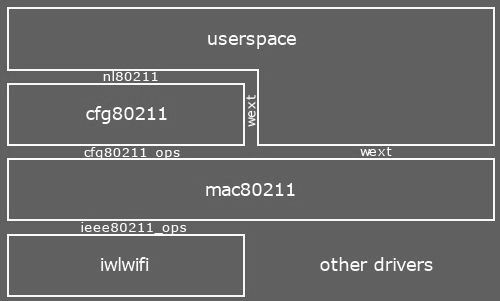
\includegraphics[width=0.9\hsize]{image201512/mac80211_arch_mono.jpg}
\caption{nl80211$B$N?^<((B}
 \end{minipage}
\end{figure}

\subsection{hostapd$B$O$I$N$h$&$K(BWLI-UC-GNM2$B$rA`:n$9$k$N$+!)(B}


  cfg8011$B$H(Bhostapd$B$ODL?.$r$7$F(BWLI-UC-GNM2$B$rA`:n$9$k$N$G$9$,!"$3$A$i$G;H$o$l$k(B
 $B%W%m%H%3%k$O!"(Blinux$B$N(BNETLINK$B$,MxMQ$5$l$^$9!#(B



%201601 kansai
\dancersection{VyOS$B$rF~$l$F(BAP$B$r9=C[$7$F$_$?!#(B}{$B$+$o$@$F$D$?$m$&(B}

\subsection{VyOS}

VyOS\footnote{\url{http://vyos.net}}$B$O(BLinux$B%Y!<%9$N%M%C%H%o!<%/%*%Z%l!<%F%#%s%0%7%9%F%`$G$9!#(B
$B%k!<%F%#%s%0!"%U%!%$%d!<%&%)!<%k!"(BVPN$B$N9=C[$K;HMQ$5$l$F$$$^$9!#(B

$B85!9$O(BVyatta$B<R$,3+H/$7$F$$$?(BVyatta Core$B$G$7$?$,3+H/85$,Gc<}$5$l$?8e$KDs6!$,=*N;$7$?$?$a!"(B
$B$3$3$+$i%U%)!<%/$73+H/$,3+;O$5$l$?$N$,(BVyOS$B$K$J$j$^$9!#(B

VyOS$B$O(BDebian$B$r%Y!<%9$K$7$F$*$j!":G?7%j%j!<%9$N(BVyOS 1.1.6 (Helium)$B$O(B
Debian 6 Squeeze$B$,%Y!<%9$H$J$C$F$$$^$9!#(B

\subsection{$B=i4|@_Dj(B}

$B%$%s%9%H!<%i$N(BISO$B%$%a!<%8$O(BLive CD$B$H$7$FDs6!$5$l$F$$$^$9$N$G(BUser Guide$B$N(BInstallation
\footnote{\url{http://vyos.net/wiki/User_Guide\#Installation}}
$B$N<j=gDL$j$K%$%s%9%H!<%k$r?J$a$^$9!#(B

$BB3$$$F%k!<%?$H$7$F;HMQ$9$k$?$a$N@_Dj$r9T$J$$$^$9!#$3$3$G$O(BUser Guide$B$N(BQuick Start Guide
\footnote{\url{http://vyos.net/wiki/User_Guide\#Quick_Start_Guide}}
$B$NDL$j$K@_Dj$7$^$9!#(B
$B$3$l$G30$HFb(B(192.168.0.1/24)$B$r7R$0%k!<%?$,$G$-$"$,$j$^$9!#(B

\subsection{$B%"%/%;%9%]%$%s%H$N9=C[(B}

$B%"%/%;%9%]%$%s%H$K;HMQ$9$kL5@~(BLAN$B%"%@%W%?$H$7$F(B
{\tt en:users:drivers [Linux Wireless]}
\footnote{\url{https://wireless.wiki.kernel.org/en/users/drivers}}
$B$r;29M$K!"(BLinux$B$,BP1~$7$F$*$j!"%"%/%;%9%]%$%s%H$H$7$FF0:n$9$k%"%@%W%?$rMQ0U$7$^$9!#(B

$B:#2s$O(BAtheros$B@=$N(BAR9280$B$r;H$$$^$9!#(B

$B$3$N%"%@%W%?$r@h$K@_Dj$7$?FbB&$N%M%C%H%o!<%/$KDI2C$9$k7A$G%"%/%;%9%]%$%s%H$r@_Dj(B
$B$7$^$9!#(B

$B<j=g$H$7$F$O%V%j%C%8$r:n@.$7$=$3$KFbB&$N%$%s%?!<%U%'!<%9(B(eth0)$B$H(B
$BL5@~(BLAN$B$N%$%s%?!<%U%'!<%9(B(wlan0)$B$rDI2C$7$^$9!#$3$N:]DI2C$9$k%$%s(B
$B%?!<%U%'!<%9$K(Baddress$B$,@_Dj$5$l$F$$$k$H%(%i!<$K$J$j$^$9$N$G@h$K(B
$B:o=|$7$^$9!#(B
\footnote{\url{http://orebibou.com/2015/01/apu1-c\%E3\%81\%AB\%E7\%84\%A1\%E7\%B7\%9Alan\%E3\%82\%A2\%E3\%83\%B3\%E3\%83\%86\%E3\%83\%8A\%E3\%82\%92\%E5\%8F\%96\%E3\%82\%8A\%E4\%BB\%98\%E3\%81\%91\%E3\%81\%A6vyos\%E3\%81\%AE\%E7\%84\%A1\%E7\%B7\%9Alan\%E3\%83\%AB\%E3\%83\%BC\%E3\%82\%BF\%E3\%83\%BC/}}

\begin{commandline}
vyos@vyos:~$ configure
vyos@vyos# delete interfaces ethernet eth1 address 192.168.0.1/24
vyos@vyos# set interfaces bridge br0
vyos@vyos# set interfaces ethernet eth1 bridge-group bridge br0
vyos@vyos# set interfaces wireless wlan0 bridge-group bridge br0
vyos@vyos# set interfaces bridge br0 address 192.168.0.1/24
vyos@vyos# commit
vyos@vyos# save
\end{commandline}
%% $

$BB3$$$F(Beth1$B$H$7$F@_Dj$7$?%5!<%S%9$r(Bbr0$B$KJQ99$7$F$*$-$^$9!#(B

\begin{commandline}
vyos@vyos# delete service dns forwarding listen-on eth1
vyos@vyos# set service dns forwarding listen-on br0
vyos@vyos# commit
vyos@vyos# save
\end{commandline}

$B$=$7$FL5@~(BLAN$B%"%/%;%9%]%$%s%H$N@_Dj$r9T$$$^$9!#(B

\begin{commandline}
vyos@vyos# set interfaces wireless wlan0 country JP
vyos@vyos# set interfaces wireless wlan0 mode g
vyos@vyos# set interfaces wireless wlan0 channel 10
vyos@vyos# set interfaces wireless wlan0 ssid vyos
vyos@vyos# set interfaces wireless wlan0 security wpa mode wpa2
vyos@vyos# set interfaces wireless wlan0 security wpa passphrase password
vyos@vyos# set interfaces wireless wlan0 type access-point
vyos@vyos# commit
vyos@vyos# save
\end{commandline}

$B$3$l$G(BIEEE802.11g$B$N%"%/%;%9%]%$%s%H$,$G$-$"$,$j$^$7$?!#(B

$B%"%/%;%9%]%$%s%H$K@\B3$G$-$J$$>l9g$O%"%/%;%9%]%$%s%H%G!<%b%s$N(Bhostapd$B$,5/F0$7$F(B
$B$$$J$$$+(Bdhcpd$B%5!<%P$,(Bbr0$B$rG'<1$7$F$$$J$$$3$H$,9M$($i$l$^$9$N$G!"$=$l$>$l$N(B
$B%G!<%b%s$r:F5/F0$7$F$/$@$5$$!#(B

$B$b$7$/$O0lEY:F5/F0$7$F$*$/$H$h$$$+$b$7$l$^$;$s!#(B

\begin{commandline}
vyos@vyos~$ sudo /opt/vyatta/sbin/hostapd-init start wlan0
\end{commandline}
%% $

\begin{commandline}
vyos@vyos~$ configure
vyos@vyos# run restart dhcp server
vyos@vyos# exit
\end{commandline}
%% $


\subsection{5GHz$BBS$H(BIEEE802.11n$B$N;HMQ(B}

$B:#2s!";HMQ$7$?L5@~(BLAN$B%"%@%W%?$O(B5GHz$BBS$H(BIEEE802.11n$B$KBP1~$7$F$$$^$9$N$G$3$l$i$r;HMQ(B
$B$G$-$k$h$&$K$7$F$_$^$9!#(B

\subsubsection{IEEE802.11a}

$B$^$:$O(B5GHz$BBS$N(BIEEE802.11a$B$N@_Dj$r9T$J$C$F$_$^$9!#(B

\begin{commandline}
vyos@vyos~$ configure
vyos@vyos# set interfaces wireless wlan0 mode a
vyos@vyos# set interfaces wireless wlan0 channel 36
vyos@vyos# commit
[ interfaces wireless wlan0 channel 36 ]
Channel 36 is not available for wlan0

[[interfaces wireless wlan0]] failed
Commit failed
[edit]
\end{commandline}
%% $

$B$H$J$j!"@_Dj$K<:GT$7$^$9!#(B

iw$B%3%^%s%I$G%A%c%s%M%k$r3NG'$9$k$H@_Dj$7$?%A%c%s%M%k$,(BBand 2$B$K$"$k$3$H$,(B
$B3NG'$G$-$^$9!#(B

\begin{commandline}
vyos@vyos:/opt/vyatta/sbin$ /usr/sbin/iw list
Wiphy phy0
	Band 1:

<snip>

	Band 2:
		Capabilities: 0x11ce
			HT20/HT40
			SM Power Save disabled
			RX HT40 SGI
			TX STBC
			RX STBC 1-stream
			Max AMSDU length: 7935 bytes
			DSSS/CCK HT40
		Maximum RX AMPDU length 65535 bytes (exponent: 0x003)
		Minimum RX AMPDU time spacing: 8 usec (0x06)
		HT TX/RX MCS rate indexes supported: 0-15
		Frequencies:
			* 5180 MHz [36] (15.0 dBm) (passive scanning, no IBSS)
			* 5200 MHz [40] (15.0 dBm) (passive scanning, no IBSS)
			* 5220 MHz [44] (15.0 dBm) (passive scanning, no IBSS)
			* 5240 MHz [48] (15.0 dBm) (passive scanning, no IBSS)

<snip>

\end{commandline}
%% $

$B$3$l$O@_Dj%9%/%j%W%H$,(BBand 2$B$N%A%c%s%M%k$r8+$F$$$J$$$?$a$G$9$N$G!"(B
$B$H$j$"$($:$3$NItJ,$rDY$7$F:FEYF1$8@_Dj$r9T$J$$$^$9!#(B

\begin{commandline}
vyos@vyos~$ configure
vyos@vyos# set interfaces wireless wlan0 mode a
vyos@vyos# set interfaces wireless wlan0 channel 36
vyos@vyos# commit
\end{commandline}
%% $

$B:#EY$O%(%i!<$J$/@_Dj$,40N;$7$^$9!#$7$+$7!"%"%/%;%9%]%$%s%H$,I=$o$l$:(B
hostapd$B%G!<%b%s$b5/F0$7$F$$$^$;$s!#(B

$B$3$l$O@_Dj$7$?%A%c%s%M%k$,!"(B{\tt (passive scanning, no IBSS)}$B$H$"$k$h$&$K!"(B
$B%Q%C%7%V%9%-%c%s>uBV$G$"$j%"%/%;%9%]%$%s%H$H$J$k$3$H$,$G$-$J$$$?$a$G$9!#(B

$B$=$3$G@_Dj%9%/%j%W%H$r:FEY=$@5$7!"%Q%C%7%V%9%-%c%s>uBV$N%A%c%s%M%k$b=|30$9$k(B
$B$h$&$K$7$^$9!#@h$N=$@5$H$"$o$;$F<!$N%Q%C%A$N$h$&$J46$8$K$J$j$^$9!#(B

\begin{commandline}
--- /opt/vyatta/sbin/wireless-config.pl.org	2016-01-23 05:09:41.455210793 +0000
+++ /opt/vyatta/sbin/wireless-config.pl	2016-01-23 05:26:43.960649746 +0000
@@ -83,10 +83,10 @@
 	while (<$iwcmd>) {
 	    chomp;
 	    next if /\(disabled\)/;
+	    next if /\(.*?(passive scanning|no IBSS).*?\)/;
 	    last unless /\* \d+ MHz \[(\d+)\]/;
 	    push @chans, $1;
 	}
-	last;
     }
     close $iwcmd;
     return @chans;
\end{commandline}
%% $

$B$3$3$^$G$N7k2L$G$O(B5GHz$BBS$G;HMQ$G$-$k%A%c%s%M%k$O0l$D$b$J$$$3$H$K$J$j$^$9!#(B

\subsubsection{$B%+!<%M%k%I%i%$%P$NJQ99(B}

{\tt en/users/Drivers/ath - Linux Wireless}$B$N(B
{\tt 5 GHz with world regulatory domain and beacon hints}
\footnote{\url{http://linuxwireless.org/en/users/Drivers/ath/\#A5_GHz_with_world_regulatory_domain_and_beacon_hints}}
$B$K$h$k$H(B5GHz$BBS$OA4$F%Q%C%7%V%9%-%c%s>uBV$H$J$C$F$$$k$h$&$G$9!#(B

$B$3$l$O3F9q!"CO0h$4$H$K;HMQ$G$-$k<~GH?tBS$,0[$J$k$?$a$@$H;W$o$l$^$9!#(B
$BF|K\$K$*$$$F$bL5@~(BLAN$B$G;HMQ$9$k(B5GHz$BBS$O!"2030$G;HMQ$G$-$k%A%c%s%M%k(B(W56)$B$H(B
$B;HMQ$G$-$J$$%A%c%s%M%k(B(W52, W53)$B!"5$>]%l!<%@$H43>D$9$k$?$a1?MQ@)8B$,$"$k(B
$B%A%c%s%M%k(B(W53, W56)$B$,$"$j$^$9!#(B

$B20Fb$G;HMQ$9$k%"%/%;%9%]%$%s%H$r9=C[$7$?$$$N$G!"$3$3$G$O20Fb$G5$>]%l!<%@$H43>D$7(B
$B$J$$%A%c%s%M%k(B(W52)$B$r%"%/%;%9%]%$%s%H$H$7$F;HMQ$G$-$k$h$&$K%+!<%M%k%I%i%$%P$rJQ(B
$B99$7$FBP1~$7$^$9!#(B

Debian$B%^%7%s>e$G(BVyOS$B$N%+!<%M%k%I%i%$%P$rJQ99$7$F%S%k%I$7$^$9!#(B

$B$^$:$O(B{\tt Rebuild VyOS kernel Step}\footnote{\url{http://vyos.net/wiki/Rebuild_VyOS_kernel_Step}}
$B$N<j=g$K=>$C$F%+!<%M%k%=!<%9%D%j!<$r<hF@$7$^$9!#(B

\begin{commandline}
$ git clone git://github.com/vyos/build-iso.git /path/to/build-iso
$ cd /path/to/build-iso
$ git submodule update --init pkgs/linux-image
$ cd checkout helium
\end{commandline}

W52$B$N%A%c%s%M%k$r%"%/%;%9%]%$%s%H$H$7$F;HMQ$G$-$k$h$&(BOpenWRT$B$N%Q%C%A(B
\footnote{\url{https://dev.openwrt.org/browser/trunk/package/kernel/mac80211/patches/403-world_regd_fixup.patch?order=name}}
$B$r;29M$K%I%i%$%P$rJQ99$7$^$9!#(B

\begin{commandline}
diff --git a/drivers/net/wireless/ath/regd.c b/drivers/net/wireless/ath/regd.c
index 1217c52..74ce3df 100644
--- a/drivers/net/wireless/ath/regd.c
+++ b/drivers/net/wireless/ath/regd.c
@@ -42,7 +42,8 @@ static int __ath_regd_init(struct ath_regulatory *reg);
 				NL80211_RRF_PASSIVE_SCAN | NL80211_RRF_NO_OFDM)
 
 /* We allow IBSS on these on a case by case basis by regulatory domain */
-#define ATH9K_5GHZ_5150_5350	REG_RULE(5150-10, 5350+10, 80, 0, 30,\
+#define ATH9K_5GHZ_5150_5350	REG_RULE(5150-10, 5240+10, 80, 0, 30, 0),\
+								REG_RULE(5260-10, 5350+10, 80, 0, 30,\
 				NL80211_RRF_PASSIVE_SCAN | NL80211_RRF_NO_IBSS)
 #define ATH9K_5GHZ_5470_5850	REG_RULE(5470-10, 5850+10, 80, 0, 30,\
 				NL80211_RRF_PASSIVE_SCAN | NL80211_RRF_NO_IBSS)
@@ -63,7 +64,7 @@ static int __ath_regd_init(struct ath_regulatory *reg);
 /* Can be used for:
  * 0x60, 0x61, 0x62 */
 static const struct ieee80211_regdomain ath_world_regdom_60_61_62 = {
-	.n_reg_rules = 5,
+	.n_reg_rules = 6,
 	.alpha2 =  "99",
 	.reg_rules = {
 		ATH9K_2GHZ_ALL,
@@ -73,7 +74,7 @@ static const struct ieee80211_regdomain ath_world_regdom_60_61_62 = {
 
 /* Can be used by 0x63 and 0x65 */
 static const struct ieee80211_regdomain ath_world_regdom_63_65 = {
-	.n_reg_rules = 4,
+	.n_reg_rules = 5,
 	.alpha2 =  "99",
 	.reg_rules = {
 		ATH9K_2GHZ_CH01_11,
@@ -84,7 +85,7 @@ static const struct ieee80211_regdomain ath_world_regdom_63_65 = {
 
 /* Can be used by 0x64 only */
 static const struct ieee80211_regdomain ath_world_regdom_64 = {
-	.n_reg_rules = 3,
+	.n_reg_rules = 4,
 	.alpha2 =  "99",
 	.reg_rules = {
 		ATH9K_2GHZ_CH01_11,
@@ -94,7 +95,7 @@ static const struct ieee80211_regdomain ath_world_regdom_64 = {
 
 /* Can be used by 0x66 and 0x69 */
 static const struct ieee80211_regdomain ath_world_regdom_66_69 = {
-	.n_reg_rules = 3,
+	.n_reg_rules = 4,
 	.alpha2 =  "99",
 	.reg_rules = {
 		ATH9K_2GHZ_CH01_11,
@@ -104,7 +105,7 @@ static const struct ieee80211_regdomain ath_world_regdom_66_69 = {
 
 /* Can be used by 0x67, 0x68, 0x6A and 0x6C */
 static const struct ieee80211_regdomain ath_world_regdom_67_68_6A_6C = {
-	.n_reg_rules = 4,
+	.n_reg_rules = 5,
 	.alpha2 =  "99",
 	.reg_rules = {
 		ATH9K_2GHZ_CH01_11,
\end{commandline}

$B$=$7$F!"%S%k%I4D6-$H$7$F(Bcowbuilder$B$G(Bsqueeze$B4D6-$rMQ0U$7$F%S%k%I$7$^$9!#(B
\footnote{\url{https://gist.github.com/hiroyuki-sato/201032fe75d2cf9f5801} \\
\url{https://gist.github.com/higebu/b4ee62b32c517b6598b2}
}

\begin{commandline}
$ sudo cowbuilder \
  --create --distribution squeeze \
  --basepath /var/cache/pbuilder/base-vyos-squeeze-amd64.cow
$ sudo cowbuilder \
  --login \
  --bindmount /path/to/build-iso \
  --basepath /var/cache/pbuilder/base-vyos-squeeze-amd64.cow/
# apt-get install devscripts kernel-package python debhelper bc
# cd /path/to/build-iso/pkgs/linux-image
# ./debian/bin/build-flavour.sh amd64-vyos
# cd ../../
# make linux-image
\end{commandline}

$B%S%k%I$,40N;$9$k$H(B/path/to/build-iso/pkgs$B0J2<$K(Bdeb$B%U%!%$%k$,@8@.$5$l$F$$$^$9$N$G(B
$B$3$N(Bdeb$B%Q%C%1!<%8$r%$%s%9%H!<%k$7$F%I%i%$%P$r99?7$7$^$9!#(B

\subsubsection{IEEE802.11a ($B:F@_Dj(B)}

$B:FEY!"(BIEEE802.11a$B$N@_Dj$r9T$J$$$^$9!#(B

$B$^$:$O(Biw$B%3%^%s%I$G(BW52$B$N%A%c%s%M%k$,%Q%C%7%V%9%-%c%s>uBV$H$J$C$F$$$J$$$3$H$r(B
$B3NG'$7$^$9!#(B

\begin{commandline}
vyos@vyos:~$ /usr/sbin/iw list
Wiphy phy0
	Band 1:

<snip>

	Band 2:
		Capabilities: 0x11ce
			HT20/HT40
			SM Power Save disabled
			RX HT40 SGI
			TX STBC
			RX STBC 1-stream
			Max AMSDU length: 7935 bytes
			DSSS/CCK HT40
		Maximum RX AMPDU length 65535 bytes (exponent: 0x003)
		Minimum RX AMPDU time spacing: 8 usec (0x06)
		HT TX/RX MCS rate indexes supported: 0-15
		Frequencies:
			* 5180 MHz [36] (15.0 dBm)
			* 5200 MHz [40] (15.0 dBm)
			* 5220 MHz [44] (15.0 dBm)
			* 5240 MHz [48] (15.0 dBm)
			* 5260 MHz [52] (17.0 dBm) (passive scanning, no IBSS, radar detection)

<snip>

\end{commandline}
%% $

$B:FEY(BIEEE802.11a$B$N@_Dj$r9T$J$($P40N;$G$9!#(B

\subsubsection{IEEE802.11n}

$BB3$$$F(BIEEE802.11n$B$K@_Dj$rJQ99$7$^$9!#(B

\begin{commandline}
vyos@vyos~$ configure
vyos@vyos# set interfaces wireless wlan0 mode n
vyos@vyos# commit
\end{commandline}
%% $

$B%(%i!<$J$/@_Dj$,40N;$7$^$9$,!"<B:]$K$O@_Dj$K<:GT$7$F$*$j%"%/%;%9%]%$%s%H(B
$B$H$7$F2TF0$7$F$$$^$;$s!#(B

{\tt hostapd.conf}\footnote{\url{https://w1.fi/cgit/hostap/tree/hostapd/hostapd.conf}}
$B$N@_DjNc$K=>$($P(BIEEE802.11n$B$r(B5GHz$BBS$G;HMQ$9$k$K$O!"(Bieee80211n=1$B$H$7$?>e$G(B
hw\_mode=a$B$H@_Dj$7$J$1$l$P$$$1$^$;$s!#(B

$B@8@.$5$l$?@_Dj%U%!%$%k(B(/var/run/hostapd/wlan0.cfg)$B$r3NG'$9$k$H(B
ieee80211n=1$B$H$J$C$F$$$^$9$,!"(Bhw\_mode=g$B$H$J$C$F$$$^$9!#(B
$B@_Dj%U%!%$%k@8@.%9%/%j%W%H$KLdBj$,$"$j$^$9$N$G=$@5$7$^$9!#(B

$B$3$N=$@5$G(B5GHz$BBS$G(BIEEE802.11n$B$O;HMQ$G$-$k$h$&$K$J$j$^$9$,!"(BIEEE802.11n$B$K$O3HD%(B
$B%b!<%I$,$"$j$^$9$N$G$G$-$l$P$3$l$b;HMQ$G$-$k$h$&$K$7$F$_$^$9!#(B

$B$7$+$7!"$I$&$d$i(BVyOS$B$O(BIEEE802.11n$B$N3HD%%b!<%I$KBP1~$7$F$$$J$$$h$&$G!"@hDx$N@_Dj(B
$B%U%!%$%k@8@.%9%/%j%W%H$K$bF~NO%$%s%?!<%U%'!<%9B&$N%9%/%j%W%H$K$bBP1~$7$?=hM}$,$"(B
$B$j$^$;$s!#(B

$B%"%@%W%?$K$"$o$;$F@_Dj$G$-$k$h$&$K=$@5$7$F$$$/$N$OBgJQ$G$9$N$G!"$3$3$G$O@_Dj%U%!(B
$B%$%k@8@.%9%/%j%W%H$KD>=q$-$9$k$3$H$GBP1~$7$^$9!#$?$@!"%A%c%s%M%k%\%s%G%#%s%0$N@_(B
$BDj$O;HMQ$9$k%A%c%s%M%k$K$"$o$;$FJQ99$9$kI,MW$,$"$j$^$9!#%A%c%s%M%k$rJQ99$9$kEY$K(B
$B%9%/%j%W%H$r=q$-49$($k$N$OBgJQ$G$9$N$G$3$NE@$K$@$1BP1~$7$F$*$-$^$9!#(B

$B$3$3$^$GBP1~$5$;$?@_Dj%U%!%$%k@8@.%9%/%j%W%H$NJQ99$O<!$N%Q%C%A$N$h$&$K$J$j$^$9!#(B
ht\_capab$B$O$4;HMQ$N%"%@%W%?$K$"$o$;$FBP1~$5$;$kI,MW$,$"$j$^$9$N$G$4Cm0U$/$@$5$$!#(B

\begin{commandline}
vyos@vyos:~$ diff -u /opt/vyatta/sbin/wireless-hostapd.pl{.org,}
--- /opt/vyatta/sbin/wireless-hostapd.pl.org	2016-01-23 08:55:16.208240635 +0000
+++ /opt/vyatta/sbin/wireless-hostapd.pl	2016-01-23 10:29:52.095371845 +0000
@@ -98,8 +98,21 @@
 
 my $hw_mode = $config->returnValue('mode');
 if ( $hw_mode eq 'n' ) {
-    print "hw_mode=g\n";
-    print "ieee80211n=1\n"
+    if ( (34 <= $chan) and ($chan <=165) ) {
+        print "hw_mode=a\n";
+    } else {
+        print "hw_mode=g\n";
+    }
+    print "ieee80211n=1\n";
+    my @CH_HT40_PLUS = qw(1 2 3 4 5 6 7 8 9 36 44 52 60);
+    my @CH_HT40_MINUS = qw(5 6 7 8 9 10 11 12 13 40 48 56 64);
+    my $ht_capab = "[SHORT-GI-40][TX-STBC][RX-STBC1][DSSS_CCK-40]";
+    if ( grep {$_ eq $chan} @CH_HT40_PLUS ) {
+        $ht_capab = $ht_capab . "[HT40+]";
+    } elsif ( grep {$_ eq $chan} @CH_HT40_MINUS ) {
+        $ht_capab = $ht_capab . "[HT40-]";
+    }
+    print "ht_capab=$ht_capab\n"
 } else {
     print "hw_mode=$hw_mode\n";
 }
\end{commandline}
%% $

$B$3$l$G!":FEY(BIEEE802.11n$B$N@_Dj$r9T$J$($P40N;$G$9!#(B

\subsection{$B$^$H$a(B}

VyOS$B$G(B2GHz$BBS$NL5@~(BLAN$B%"%/%;%9%]%$%s%H9=C[$O4JC1$K$G$-$^$9!#(B

$B$7$+$7!"(B5GHz$BBS$d(BIEEE802.11n$B$r;HMQ$9$k>l9g$O>/$7<j4V$G$9!#(B
$B%9%/%j%W%H$NLdBj$O(BVyOS$B8GM-$NLdBj$G$9$,!"%I%i%$%P$K$D$$$F$OB>$N(BLinux$B%G%#%9%H%j%S%e!<(B
$B%7%g%s$G$bF1$8LdBj$KD>LL$9$k$H;W$$$^$9!#(B{\tt en:users:drivers [Linux Wireless]}
$B$J$I$r;29M$KLdBj$N>/$J$$L5@~(BLAN$B%"%@%W%?$r;HMQ$9$k$3$H$,9=C[$N6aF;$+$H;W$$$^$9!#(B

%201601 kansai $B<}O?L5$7(B
%GNUHurd$B$N%$%s%9%H!<%k$7$F$_$?!#$H!"(BX$B%5!<%P$NN)$A>e$2$KD)@o(B $B@n9>(B $B9@(B
%GNUHurd$B$K$D$$$F$O!"869F$O:n$C$F$J$$$N$G!":#2s$O%Q%9$H$N$3$H!#(B

%201605 tokyo
%-------------------------------------------------------------------------------
\dancersection{Buffalo Linkstation $B8~$1(B Debian Installer}{Roger Shimizu}
%-------------------------------------------------------------------------------

\subsection{$B;O$a$K(B}
VGA/HDMI port $B$d(B Keyboard $B$J$IIU$$$F$J$$5!4o!"Nc$($P%5!<%P8~$1$F(BPC$B!"$=$l$+$i(B ARM $B3+H/%\!<%I$J$I$N5!4o$K!"$I$&$d$C$F(B Debian $B$rF~$l$F$*$/$G$7$g$&$+!)(B
RAID $BIU$-$N(B Buffalo Linkstation NAS $B$rNc$H$7$F!">R2pCW$7$^$9!#(B

\subsection{Buffalo Linkstation $B$NNr;K(B}

\begin{itemize}
\item $BBh#0@$Be(B: Linkstation / Kuro-Box
\item $BBh#1@$Be(B: Linkstation HG / Kuro-Box HG
	\begin{itemize}
	\item PowerPC architecture
	\item IDE/PATA $B$N$_(B (SATA $B$,$J$7(B)
	\item $B8=:_$"$C$F$b;H$$$E$i$$$H;W$$$^$9(B
	\end{itemize}
\item $BBh#2@$Be(B\footnote{MIPS$B$N(BModel$B$b=P$?$1$l$I!"(BModel$B?t$,>/$J$$$7!"=P$F$9$0%G%9%3%s$K$J$C$F$7$^$C$?$N$G!"$3$A$i>JN,$5$;$FD:$-$^$9!#(B}: 
Kuro-Box Pro / Linkstation Live / Linkstation LS-GL/LS-WTGL/LS-WSGL/LS-QL
	\begin{itemize}
	\item ARM architecture
		\begin{itemize}
		\item Debian Etch$B$^$G(B: arm OABI (Old ABI)
		\item Debian Lenny$B$+$i(B: armel EABI (new Embedded ABI)
		\end{itemize}
	\item Marvell orion5x 5182 chipset; SATA interface
	\end{itemize}
\item $BBh#3@$Be(B: Linkstation LS-XHL/LS-CHL/LS-WXL \& Linkstation LS-VL/LS-WVL/LS-QVL, etc
	\begin{itemize}
	\item Marvell kirkwood 6281 / 6282 chipset
	\item armel architecture $B$J$N$G!"Bh#2@$Be$H(B rootfs $B$N8_49@-$,$"$j!"$^$?(B Debian Kernel 4.4 $B$+$iF1$8!V(B-marvell$B!W$H$N(B flavour $B$G6&DL$KBP1~$5$l$^$9!#(B
\footnote{HDD$B$r0[$J$k7?HV$N5!4o$KF~$l$kA0$K!"(Bflash-kernel$B$GE,@Z$J(BDTB$B$r(BuImage.buffalo$B$KF~$lCV$+$J$$$H9T$1$^$;$s!#(B}
	\end{itemize}
\item $BBh#4@$Be(B: LS-210/LS-220/LS-410/LS-420, etc
	\begin{itemize}
	\item Marvell armada-370 chipset
	\item armhf architecture (hard-float)
	\item $B;DG0$J$,$i!"(BLinux Kernel $B$NJ}$,$^$@BP1~$5$l$F$J$$$h$&$G$9!#(B
	\end{itemize}
\end{itemize}

\subsection{Debian Installer $B$N>R2p(B}

\begin{itemize}
\item Debian Installer ($BN,$O(B D-I $B$H$J$j$^$9(B)$B$G$O!"MM!95!4o$K(B Debian $B$r%$%s%9%H!<%k$7$F$/$l$k%D!<%k$H$J$j$^$9!#(B
	\begin{itemize}
	\item $BHs(B Linux $B$J(B OS $B$G$bBP1~$5$l$k!"Nc$((B kFreeBSD $B$d(B GNU/Hurd $B$J$I(B
	\item $B%a%G%#%"$O(B CD/DVD $B$K8B$i$l$:!"(BPXE netboot $B$d(B u-boot $B$J$IMM!9=@Fp$J%$%s%9%H!<%k%a%G%#%"$rDs6!$5$l$F$*$j$^$9!#(B
	\item $B%b%K%?!<$J$II=<(%G%P%$%9$,IU$$$F$J$$5!4o$G$bBP1~$5$l$k(!(!(Bnetwork-console $B%$%a!<%8(B\\
	$B!!"M(B $B$A$g$&$I(B Buffalo Linkstation $B$J$I(B NAS $B5!4o$K8~$1(B
	\end{itemize}
\item $B8=:_(B D-I $B$KBP1~$5$l$F$$$k(B Linkstation $B%j%9%H(B\footnote{d-i daily image $B$,4^$^$l$k(B}:
	\begin{itemize}
	\item Kuro-Box Pro / Linkstation Pro/Live
	\item Linkstation LS-GL / LS-WSGL / LS-WTGL
	\item Linkstation LS-XHL / LS-CHLv2 / LS-WXL / LS-WSXL / LS-VL / LS-WVL / LS-QVL\\
	$B!!"M(B armel $B$NBh#2@$Be$HBh#3@$Be$O$[$H$s$IBP1~$5$l$F$^$9(B
	\end{itemize}
\end{itemize}

\subsection{Linkstation$B$X(B Debian $B$N(B $B%$%s%9%H!<%k;EJ}(B}

\subsubsection{Linkstation $B$K(B Debian Installer $B$r5/F0$5$;$k(B}
Buffalo Linkstation $B$G$O!"(Bu-boot $B$H$$$&(B boot loader $B$,!"(B1$BHVL\$N(B partition (/dev/sda1 $BKt$O(B /dev/md0) $B$KJ]B8$5$l$k(B kernel $B$H(B initrd $B$rFI$_9~$s$G5/F0$r9T$$$^$9!#(B
$B$=$l$+$i!"(BD-I $B%$%a!<%8$r(B1$BHVL\$N(B partition $B$KCV$$$H$1$P!"(BDebian Installer $B$,5/F0$5$l$^$9!#(B
$B<j=g$O2<5-$NDL$j$H$J$j$^$9!#(B
\begin{itemize}
\item 1$BHVL\$N(B partition $B$r%U%)!<%^%C%H$9$k(B\footnote{1$BHVL\$N(B partition $B$O(B ext2/ext3 $B$K8B$i$l$^$9!#(B}($B4{$KB8:_$9$k$J$i>JN,2D(B)
\item D-I kernel/initrd $B%$%a!<%8$r!"(B1$BHVL\$N(B partition $B$K%3%T!<$9$k!#(BD-I $B%$%a!<%8$O2<5-(BURL$B$G%@%&%s%m!<%I=PMh$^$9!#(B
	\begin{itemize}
	\item https://d-i.debian.org/daily-images/armel/daily\\/orion5x/network-console/buffalo
	\item https://d-i.debian.org/daily-images/armel/daily\\/kirkwood/network-console/buffalo
	\end{itemize}
\item D-I kernel/initrd image $B$rF~$l$?(B HDD $B$r(B Linkstation $B$K<h$jIU$1$^$9!#(B
\item Linkstation $B$r5/F0$7!"(BDHCP $B$G(B IP Address $B$r3d$jEv$F$i$l$k$^$G;C$/BT$C$F!"$=$l$+$i3d$jEv$F$i$l$?(B IP Address $B$K(B SSH $B$G@\B3$7$^$9!#(B
\item $B2hLL$K1h$C$F!"DL>o$J(B Debian Install $B9T$&$3$H$,=PMh$^$9!#(B
\end{itemize}

\subsubsection{$B>\:Y$J<j=g(B: HDD Partition $B$N:n@.(B}
Linkstation$B$N(BHDD$B$r(BLinkstation$B$+$i30$7!"(BSATA-USB$B%"%@%W%?!<$J$IJ}K!7PM3$G(BPC$B$K@\B3$7$^$9!#Nc$($P!"$=$N(B HDD $B$,(B /dev/sdc $B$H$7$F@bL@$7$^$9!#(B
LS-WXL/WSXL/WVL/QVL $B$J$I(B RAID $B5!4o$N>l9g$O!"$9$Y$F$N(B HDD $B$rF1$8(B partition $B$K$7$F$bNI$$$G$9!#(B
\begin{commandline}
$ sudo parted /dev/sdc
(parted) mklabel gpt
(parted) mkpart boot 2048s 1024MiB
(parted) mkpart root 1024MiB 6144MiB
(parted) mkpart swap 6144MiB 6400MiB
(parted) mkpart data 6400MiB -1
# $B2<5-$N%3%^%s%I$O(B RAID $B9=@.$N5!<o$@$1I,MW$H$J$j$^$9!#(B
(parted) set 1 raid on
(parted) set 2 raid on
(parted) set 3 raid on
(parted) set 4 raid on
\end{commandline}

\subsubsection{$B>\:Y$J<j=g(B: HDD Partition $B$N3NG'(B}
\begin{itemize}
\item Partition $B$r:n$C$?$i!"3NG'$9$k$H$3$&$J$j$^$9!#(B
\end{itemize}
\begin{commandline}
(parted) print
Model: SAMSUNG HM250HI (scsi)
Disk /dev/sdc: 250GB
Sector size (logical/physical): 512B/512B
Partition Table: gpt
Disk Flags:
Num Start   End     Size    File sys  Name  Flags
 1  1049kB  1074MB  1073MB            boot  raid
 2  1074MB  6442MB  5369MB            root  raid
 3  6442MB  6711MB  268MB             swap  raid
 4  6711MB  250GB   243GB             data  raid

# $B:G8e$K(Bparted$B$r=*N;$5$;$^$9!#(B
(parted) quit
\end{commandline}
\begin{itemize}
\item RAID $B9=@.$N>l9g$OB>$N(B HDD $B$bF1$8$h$&$K%;%C%H$7$F$/$@$5$$!#(B
\end{itemize}

\subsubsection{$B>\:Y$J<j=g(B: boot image $B$N%;%C%H(B}
\begin{itemize}
\item boot image kernel/initrd $B$rBh#1HVL\(B partition $B$K%3%T!<$7$^$9!#(B($BNc$(!"(BLS-WXL $B$N%$%a!<%8(B)
\item RAID $B$NJ#?t(BHDD$B$N>l9g$O!"G0$N$?$a$9$Y$F(BHDD$B$r%3%T!<$7$^$7$g$&!#(B\footnote{$B$3$N;~E@$K!V(Bmdadm --create$B!W$G(B RAID $B$N9=@.$r$7$J$/$F$bNI$$$G$9!#(BInstall$B$N:]$K(B RAID $B$N:n@.$r9T$$$^$9!#(B}
\end{itemize}
\begin{commandline}
$ sudo mkfs.ext3 /dev/sdc1
$ sudo mount /dev/sdc1 /mnt
$ wget https://d-i.debian.org/daily-images/armel\
  /daily/kirkwood/network-console/buffalo/ls-wxl\
  /uImage.buffalo
$ wget https://d-i.debian.org/daily-images/armel\
  /daily/kirkwood/network-console/buffalo/ls-wxl\
  /initrd.buffalo
$ sudo cp *.buffalo /mnt
$ sudo umount /mnt
\end{commandline}

\subsubsection{$B>\:Y$J<j=g(B: SSH $B$G@\B3(B}
\begin{itemize}
\item HDDs $B$r(B Linkstation $B$KLa$7$F!"5/F0$5$;$^$9!#(B
\item $B;C$/BT$D$H!"(BAndroid/iOS $B%"%W%j!V(BFing$B!W$N$h$&$J(B IP/port scanner $B$G(B Linkstation $B$K3d$jEv$F$?(B IP $B$r8+$D$1$^$9!#$^$?!"(BDHCP $B%5!<%PB&$N%m%0$G$b(B
\item IP $B$rJ,$+$k$H!"(BSSH $B%3%^%s%I$rC!$/$H(B debian installer $B2hLL$,=P$FMh$k!'(B
\end{itemize}
\begin{commandline}
$ ssh installer@<IP address of Linkstation>
\end{commandline}
\begin{itemize}
\item D-I $B$N%G%U%)%k%H%Q%9%o!<%I$O!V(Binstall$B!W$H$J$j$^$9!#(B
\item command line $B$GA`:n$d(B log $B3NG'$J$I$N$?$a!"$b$&0lK\(B SSH $B$r@\B3$7$F$bNI$$$G$9!#(B
\end{itemize}

\subsubsection{RAID $B9=@.8~$1(B Install $B;~$NCm0U;v9`(B}
\begin{itemize}
\item LS-GL/CHL/XHL/VL $B$J$I(BRAID$B9=@.$G$O$J$$5!<o$@$H%9%-%C%W$/$@$5$$!#(B
\item $B$b$7(B RAID $B$N@_Dj$,8+$D$+$i$J$$>l9g$O!"(BD-I Partman $B$N2hLL$+$i0lC6!V%P%C%/!W$7!"!V(BDownload installer components$B!W$K(B partman-md $B$d(B sata-modules $B$J$I%b%8%e!<%k$rA*Br$7$F$+$i!"=PMh$k$h$&$K$J$j$^$9!#(B
\item $B$b$7(B D-I $B$G(B RAID $B$r?75,$K:n@.$9$k>l9g!"0lHVL\$N(B /dev/md0 $B$O(B metadata=0 (version 0.90) $B$K@_Dj$7$J$$$H:F5/F0$7$J$/$J$j$^$9!#860x$O(B u-boot $B$,Bh#1HVL\(B partition $B$N(B kernel/initrd $B$rFI$_9~$^$J$/$J$k$?$a!#8=:_(B partman-md $B$K@_Dj=PMh$J$/$F(B\footnote{\url{https://bugs.debian.org/815569}}$B!"(Bcommand line $B$K$7$^$7$g$&!'(B
\begin{commandline}
# mdadm --create /dev/md0 --level=1 --raid-devices=2 \
  --metadata=0 /dev/sda1 /dev/sdb1
\end{commandline}
\item $B$^$?$O(B ($BB>$N(B HDD $B$,8e$K$7$^$9(B)
\begin{commandline}
# mdadm --create /dev/md0 --level=1 --raid-devices=2 \
  --metadata=0 /dev/sda1 missing
\end{commandline}
\item /dev/md0 $B0J30$N(B RAID $B$O(B partman-md $B$G@_Dj$7$F$bNI$$$G$9!#(B
\item RAID $B$r?75,$K:n@.$9$k(B (create) $B$HF14|2=$N:n6H$,$9$0$K;O$a$5$l!"$H$F$b=E$/$F!"?J9TCf(B Debian Install $B$N:n6H$K1F6A$J$i$J$$$h$&$K(B /dev/md0 $B0J30$NF14|2=$NB.EY$r@)8B$+$1$?J}$,NI$$$G$9!'(B
\end{itemize}
\begin{commandline}
# echo 100 > /sys/block/md{1,2,3}/md/sync_speed_max
\end{commandline}
\begin{itemize}
\item $B%$%s%9%H!<%k$,=*$o$C$F:F5/F0$7$?$i!"(BRAID $B$NF14|2=$N:n6H$O<+F0E*$K:F3+$5$l$k$N$G!"$=$N8e$N:n6H$OFC$KI,MW$"$j$^$;$s!#(B
\end{itemize}

\subsubsection{Debian Install $B8e$N@_Dj(B}
\begin{itemize}
\item u-boot $B4D6-JQ?t$r3NG'!&JQ99$N$?$a!"%3%^%s%I(B fw\_printenv / fw\_setenv $B$N@_Dj(B
\footnote{u-boot $B4D6-JQ?t$rJQ99$9$k$H5/F0$7$J$$>l9g$,$"$j!"=$I|<jCJ$,$"$^$j$J$/$F!"5$$r$D$1$^$7$g$&!#(B}
	\begin{itemize}
	\item $B$[$H$s$I$N5!<o$O2<5-$N@_Dj$,:Q$_$G$9!'(B
	\end{itemize}
\begin{commandline}
$ sudo echo /dev/mtd2 0x00000 0x10000 0x10000 \
	> /etc/fw_env.config
\end{commandline}
	\begin{itemize}
	\item Kuro-Box Pro $B$O(B mtd/flash $B$N?t$,0[$J$k$N$G!"2<5-$N@_Dj$K$7$F$/$@$5$$!#(B
	\end{itemize}
\begin{commandline}
$ sudo echo /dev/mtd5 0x00000 0x10000 0x10000 \
	> /etc/fw_env.config
\end{commandline}
\item $BB>$N5!4o$G(B Linkstation $B$N5/F0%m%0$r3NG'$9$k$?$a(B($B$"$k$$$O!":F5/F0ITG=$N:]$K%G%P%C%0<jCJ$H$7$F(B)$B!"(Bnetconsole $B$N@_Dj(B
	\begin{itemize}
	\item Linkstation $BB&$N@_Dj!'(B
	\end{itemize}
\begin{commandline}
$ sudo cat << EOT >> /etc/initramfs-tools/modules
marvell
mv643xx_eth
netconsole netconsole=@192.168.11.5/,6666@192.168.11.1/
mvmdio
EOT

$ sudo update-initramfs -u
\end{commandline}
	\begin{itemize}
	\item $BB>$N5!4o$G%m%0<}=8$9$k%3%^%s%I!'(B
	\end{itemize}
\begin{commandline}
$ sudo ip a add 192.168.11.1/24 dev eth0
$ nc -l -u -p 6666 | tee ~/netconsole.log
\end{commandline}
\end{itemize}


\subsection{$B=*$o$j$K(B}

Kernel $B$N(B Device-Tree $B$rBP1~$7$?$j!"(BDebian-Installer $B$K%Q%C%A$rEj$2$?$j!"(BLinkstation $B$K(B Debian Install $B$O$d$C$H=PMh$k$h$&$K$J$j$^$7$?!#(B
$B:#8e$O(B Debian Installer $B$r0z$-B3$-2~A1!&?J2=$r9T$C$F9T$-$?$$$H;W$$$^$9!#(B
\begin{itemize}
\item Debian Installer $B$K(B GNU/screen $BKt$O(B tmux $B$rBP1~$9$k(B
\footnote{\url{https://lists.debian.org/debian-boot/2016/02/msg00547.html}}\footnote{\url{https://bugs.debian.org/819397}}\footnote{\url{https://bugs.debian.org/819988}}
	\begin{itemize}
	\item SSH $B@\B3$,@Z$l$F$b!"(Binstaller $B$,%P%C%/%0%i%&%s%I$K2s$;$F!"(BSSH $B$G:F@\B3$9$k$H85$N>uBV$K:F3+$G$-$^$9!#(B
	\item $B%7%'%k$d%m%0$J$I$h$jJXMx$K%"%/%;%9=PMh$^$9!#(B
	\end{itemize}
\item partman-md $B$X(B RAID $B$N(B metadata $B;XDj$G$-$k$h$&$K!"BP1~$9$k(B\footnote{\url{https://bugs.debian.org/815569}}$B!#(B
\item $BBh#4@$Be!"(Barmhf/armada-370 $B$N(B Linkstation $B$rBP1~$9$k(B
\end{itemize}

%201602 tokyo
\dancersection{tilegx$B$H$$$&(BCPU$B%"!<%-%F%/%A%c8~$1$N(BDebian$B%Q%C%1!<%80\?"(B}{wskoka}

\subsection{$B$O$8$a$K(B}

\subsubsection{tilegx $B$C$F$J$s$@(B}
Tilera$B<R$,3+H/$7$?%M%C%H%o!<%/MQES$K@_7W$5$l$?%^%k%A%3%"(BCPU$B$N$3$H!#(B
$BB?$/$O%[%9%H%5!<%P$K(BPCI-E$B%\!<%I$rAuCe$7$F%"%/%;%i%l!<%?$N$h$&$K;H$&!#(B
$B%0%l!<%I$O(B9,16,36,72$B%3%"$,$"$j$=$l$>$l(B24,28,40,80Gbps$B$NE>AwB.EY$r;}$D!#(B
PCI-E$B$N%$%s%?!<%U%'%$%9$OEE8;6!5k$,%a%$%s$G@)8f$O%[%9%H(BOS$B$+$i9T$&!#(B
CPU-ASIC$B$N4X78$K6a$$!#(B
$B%\!<%IFb$G$OFHN)$7$F(BRedHat$B$N(BOS$B$,5/F0$7$F$$$k$i$7$$!#(B
$B%"%W%j$O>&MQ$N3+H/%D!<%k(B(MDE)$B$rMQ$$$F:n@.$9$k!#(B
$BHs>o$K9b2A$J$?$a0lHL$KN.DL$9$k$3$H$O$[$H$s$IL5$$!#(B
Linux$B%+!<%M%k$,%5%]!<%H$5$l$F$$$F!"%/%m%9%3%s%Q%$%kMQ$N(BGCC$B$,%U%j!<$G8x3+$5(B
$B$l$F$$$k!#(B
$B%"!<%-%F%/%A%cL>$O!V(Btilegx$B!W(B $B!#(B
NIC$B$N%G%P%$%9%I%i%$%P$O(BCPU$B0MB8$H$J$k$?$a%+!<%M%k$K$O4^$^$l$J$$!#(B
$BDL>o$O3+H/%D!<%k$N4D6-$K<BAu$5$l$F$$$k$b$N$r;H$&!#(B
2015$BG/(B12$B7n$K(BQEMU$B$G%5%]!<%H$5$l$?!#(B 

\subsubsection{$B$J$K$,$$$$$N(B}
ASIC$B$J$I$G$NB.EY8~>e$O;H$($k5!G=$K@)8B$,$"$k$?$aF0E*$J4D6-$K$O(B
$BIT8~$-$G(BFPGA$B$J$I$rMxMQ$9$kI,MW$,$"$k!#(B
$B$^$?!"%5!<%P(BOS$B$G2TF/$7$F$$$k%"%W%j%1!<%7%g%s$NDL?.$O%[%9%H(BCPU,$B%P%9(B,
$B%$%s%?!<%U%'%$%9$J$I2p$7$F9T$&$?$aB.EY%\%H%k%M%C%/$,H/@8$7$d$9$/9bB.(B
$B$KDL?.$9$k$?$a$K$O9b2A$JIt:`$r$=$m$($kI,MW$,$"$k!#(B
$B$9$Y$F$r%=%U%H%&%'%"$G@)8f$79bB.$JDL?.$r9T$($k$h$&$K@_7W$5$l$?(BCPU
$B$J$iBgNL$N%H%i%U%#%C%/=hM}$r=@Fp$KBP1~$G$-$k!#(B 

\subsubsection{$B<B5!$O$I$3$K(B}
$B$4$/0lIt$NBeM}E9$GHNGd$5$l$F$$$k$,!"$[$H$s$I$,>&MQ$N3+H/4D6-$J$?(B
$B$a%i%$%;%s%9NA$,2C;;$5$l$FHs>o$K9b2A$J5!:`$H$J$C$F$$$k!#(B
$B$=$NB>!"NL;:%b%G%k$N%k!<%?$H$7$FHNGd$5$l$F$$$k5!<o$,$"$k!#(B 

\subsubsection{$B%*!<%W%s%=!<%9$K$J$i$J$$$N(B}
GCC$B$,%a!<%+!<$+$i8x3+$5$l$F$$$k$N$G!"(BLinux$B%+!<%M%k$d3F<o%*!<%W%s(B
$B%=!<%9$N%"%W%j%1!<%7%g%s$r%S%k%I$9$k$3$H$O2DG=!#(B
$B$7$+$7<B9T4D6-$,$[$H$s$IB8:_$7$J$$$N$G>&MQ0J30$K:n$i$l$k$3$H$,$J(B
$B$$!#(B
$B3+H/4D6-(B(MDE)$B$r;H$C$F:n@.$7$?$b$N$O>&MQ%i%$%;%s%9$,E,MQ$5$l$k$?(B
$B$a0lHL$K8x3+$5$l$k$3$H$O$J$/!"(Btilegx$B$r%5%]!<%H$7$?4D6-$O$^$@$J$$$,(B
QEMU$B$,BP1~$7$?$3$H$K$h$j:#8e$K4|BT$,$G$-$k!#(B 

\subsubsection{OS$B4D6-$C$F$I$&$d$C$F:n$k$N(B}
x86\_64$B$N(BOS$B$G%/%m%9%3%s%Q%$%k$9$k$3$H$+$i;O$a$^$9!#(B
$B:G=i$O%+!<%M%k$G<!$K3F<o%i%$%V%i%j$H3+H/%D!<%k%A%'!<%s%V!<%HItJ,$O(B
BusyBox$B$r;H$&$HJXMx!#(B
$B6qBNE*$K$O(Bglibc,busybox,binutils,zlib,gcc,make,bash,tar,perl...$B$J$I$N$9$Y(B
$B$F$r%=!<%9$+$i%S%k%I$9$k$3$H$K$J$k!#(B
$B$"$kDxEYI,MW$J%D!<%kN`$,B7$&$H%M%$%F%#%V%3%s%Q%$%k$,2DG=!#(B
$BA4It$N0MB84X78$r2r7h$G$-$k$^$G$K$O$+$J$j$NNL$,I,MW!#(B 

\subsubsection{$B:G>.$N%V!<%H%7!<%1%s%9(B}
$B%+!<%M%k$,5/F0$7$F$+$i%m%0%$%s%W%m%s%W%H$NI=<($^$G$O(B
$B%+!<%M%k=hM}40N;(B  $B"*(B /sbin/init $B"*(B /etc/inittab $B"*(B /etc/rc $B"*(B login
$B$N$h$&$JN.$l$K$J$k!#(B
inittab$B$K%3%s%=!<%k@\B3$N%Q%i%a!<%?$H(Brc$B$X$N%j%s%/$r5-=R$7(B
init$B$KEO$5$l(Brc$B$N%9%?!<%H%"%C%W=hM}$r9T$C$?8e$K(Blogin$B$G%W%m%s%W%H$,I=<((B
$B$5$l$k!#(B
init$B$H(Blogin$B$O(Bbusybox$B$GBeMQ2DG=!#(B 

\subsubsection{$B%=!<%9$+$i$7$+%$%s%9%H!<%k$G$-$J$$$N(B}
$B:G=i$O$=$&$9$k$7$+$"$j$^$;$s$,%S%k%I:Q$_$N4D6-$r(B
$B%Q%C%1!<%82=$7$F:FMxMQ$9$k$3$H$O2DG=!#(B
configure,make,make  install $B$,L5;v$KDL$C$?$i(B
make install DESTDIR=[$B%G%#%l%/%H%j(B] 
$B$GCj=P$7$?%G!<%?$r05=L$7$FJ]B8$9$k$3$H$,$G$-$k!#(B
rpm$B$d(Bdeb$B$J$I$N%Q%C%1!<%8$K$9$k$K$OB?$/$N%D!<%k$,I,MW$G(B
$BFC$K(Brpm$B%Q%C%1!<%8$r:n$k$?$a$N%3%^%s%I(B(rpmbuild)$B$r:n@.$9$k$K$O(B
$BFq0WEY$,9b$$$,(Bdeb$B%Q%C%1!<%8$J$iHf3SE*MF0W$K:n$k$3$H$,$G$-$k!#(B 

\subsubsection{deb$B%Q%C%1!<%8$N$D$/$j$+$?$O(B}
$B@5<0$K$O(BDebian $B?7%a%s%F%J!<%,%$%I$K=q$+$l$F$$$kDL$j$NJ}K!$G(B
$B8x<0%5%$%H$+$i%=!<%9$r%@%&%s%m!<%I$7$F2rE`$7(Bdpkg-buildpackage$B$G%S%k%I$9$k!#(B
$B$7$+$7(Btilegx$B$N(Bdebian$B4D6-<+BN$,L5$/(Bdpkg-buildpackage$B$,:G=i$O;H$($J$$$N$G(B
dpkg$B$r%=!<%9$+$i%$%s%9%H!<%k$9$kI,MW$,$"$k!#(B
dpkg$B$r%S%k%I$9$k$H$-$K(Bcputable$B$K(Btilegx$B$rDI2C$9$k!#(B
$B$3$l$r$d$i$J$$$H(Bunknown architecture$B$H$J$C$F$7$^$$%S%k%I$,=PMh$F$b(B
$B$[$H$s$I$,IT40A4$J$b$N$K$J$k!#(B
$B$3$l$K$h$j!V(Btilegx-linux-gnu$B!W$H$7$F07$&$h$&$K$J$k!#(B
$B8x3+$5$l$F$$$k%/%m%9%3%s%Q%$%kMQ$N(BGCC$B$O!V(Btilegx-unknown-linux-gnu$B!W(B
$B$H$J$C$F$$$k$?$a$3$l$H6hJL$9$kI,MW$,$"$k!#(B 

\subsection{$B%U%k%9%/%i%C%A(B}
\subsubsection{GCC$B$NF~<j(B}
$B%a!<%+%5%$%H$+$i(Btilegx-x86\_64.tar.bz2$B$r%@%&%s%m!<%I$7$F2rE`$7$?$i(B
tilegx-x86\_64$B$H$$$&%U%)%k%@$K%D!<%k%A%'!<%s0l<0$,$"$k!#(B
$B%G%#%l%/%H%j$r4D6-JQ?t$K@_Dj$9$l$P%/%m%9%3%s%Q%$%k$,2DG=!#(B
\begin{commandline}
PATH=$PATH:/usr/src/tilegx-x86_64/bin/export
LD_LIBRARY_PATH=/usr/src/tilegx-x86_64/lib 
\end{commandline}

\subsubsection{$B%+!<%M%k%3%s%Q%$%k(B}
$B%*%U%#%7%c%k$N!V(BLinux Kernel Archives$B!W$+$i%+!<%M%k%=!<%9$r(B
download$B$7(Bconfig$B$r@_Dj$7$?$i%S%k%I3+;O!#(B
\begin{commandline}
make ARCH=tilegx menuconfig
make ARCH=tilegx CROSS_COMPILE=tilegx-unknown-linux-gnu-
\end{commandline}
$B40Av8e$K=P$F$-$?(Bvmlinux$B$,5/F0MQ$N%+!<%M%k$H$J$k!#(B
NAND$B=q$-49$(MQ$K(Binitramfs$B$r(Bram$B%I%i%$%V$+$i5/F0$5$;$k$b$N$H(B
$B30It%9%H%l!<%8$d(BNAND$B%I%i%$%V$+$iDL>o5/F0$5$;$k$b$N$,I,MW!#(B
$BFC$K;XDj$,$J$1$l$P:G8e$K(B/sbin/init$B$X=hM}$,0z$-EO$5$l$k!#(B
$B8e$KI,MW$J%+!<%M%k%X%C%@$b:n$C$F$*$/!#(B 

\subsubsection{$B%f!<%6!<%i%s%I$N:n@.(B}
OS$B5/F0MQ$N(Brootfs$B4D6-$r9=C[$9$k$?$a:GDc8BI,MW$J$b$N$O(B
$B3F<o%k!<%H%G%#%l%/%H%j$H%Q%9%o!<%I%U%!%$%k$d%G%P%$%9>pJs$rI=<($9$k$?(B
$B$a$N%7%s%\%j%C%/%j%s%/$"$H$O5/F0$KI,MW$J<B9T%U%!%$%kN`!#(B
\begin{commandline}
mkdir -p bin root dev sys ram lib mnt tmp etc/lib sbin usr var proc opt var/opt var/tmp usr/share usr/share/lib mnt home 
touch etc/passwd etc/shadow etc/gshadow etc/group etc/fstab etc/inittab etc/rc
ln -s /proc/mounts etc/mtab 
\end{commandline}
$B%+!<%M%k%X%C%@(B,BusyBOX$BK\BN$H%3%^%s%IMQ%7%s%\%j%C%/%j%s%/$rG[CV!#(B
\\
inittab$B$K$O!V(B::sysinit:/etc/rc$B!W$H(B
$B!V(Bconsole::respawn:/sbin/getty  -L 115200 console$B!W$J$I$r=q$$$F$*$/!#(B
BusyBOX$B$r;H$&$H%m%0%$%sItJ,$d0lHLE*$J%3%^%s%I3F<o$,;H$($k$?$aJLES(B
$B%i%$%V%i%j$H%P%$%J%j$rG[CV$9$l$P:GDc8B$N<B9T4D6-$H$7$FF0:n$9$k!#(B 

\subsubsection{$B%M%$%F%#%V%3%s%Q%$%k4D6-$N@0Hw(B}
$B?7$?$K5/F0$7$?4D6-$G%S%k%I$r9T$&$?$a$KI,MW$J$b$N$O%/%m%9%3%s%Q%$%k(B
$B$G:n$C$F$*$/!#(B 
\\
gcc, glibc, make, binutils, zlib
\\
$B$J$I$,$"$l$P(B
\\
bash, tar, xz, gcc, sed, patch, bzip2, unzip60, perl, m4, libtool, binutils, gmp, ncurses, texinfo, gettext, coreutils, newlib, libelf, libiconv, flex, bison, libpcap, libpipeline, attr, libcap, libxml2, pth, libgpg-error, libassuan, libksba, libffi, npth, gawk, pkg-config, glibc, expat, Python, autoconf, automake, git, glib, file, openssl, readline, lua, termcap, gdb, cmake, libgcrypt, gnupg, libssh2, Linux-PAM, shadow, cracklib, libsocket, prngd, openssh, tcl, tk, sqlite-autoconf, vim, acl, curl, bind, util-linux, dhcp, ntp, bc, inetutils, kmod, rsync, nettle, gnutls, wget, apr, apr-util, pcre, libtirpc, libevent, libnfsidmap, rpcbind, LVM, nfs-utils, fuse, gperf, parted, boost, dovecot, at, subversion, icu, llvm, gsl, zabbix, httpd, php, mysql, nspr, nss, cpio, popt, libarchive, BerkeleyDB, rpm, expect, bridge-utils, otp, LINC, dropbear, lagopus, eudev, SoftEther, nginx, php-fpm, webmin
\\
$B$H$$$C$?=gHV$G%S%k%I(B/$B%$%s%9%H!<%k$9$k$3$H$,$G$-$?!#(B 
configure$B$N0z?t$O$[$\(Bprefix=/usr$B$K$J$k$,Nc30$b$"$k$N$G(B
Linux from Scratch\footnote{\url{http://www.linuxfromscratch.org/} \url{http://lfsbookja.osdn.jp/}}$BEy$r;29M!#(B

$B$*$*$h$=$3$NJU$j$^$GE~C#$9$k$H<+A0$G%+!<%M%k$,%3%s%Q%$%k$G$-$k$h$&(B
$B$K$J$k!#(B 
\subsection{Debian$B0\?"(B}
\subsubsection{$B0\?"$N%a%j%C%H(B}
$B<B9T4D6-$rMQ0U$9$k$?$a$KETEY%=!<%9$+$iF~$l$F$$$?$N$G$O(B
$BMxMQHO0O$,@)8B$5$l$k$?$a%Q%C%1!<%8$+$i<j7Z$KF3F~$G$-$k4D6-$,(B
$BI,MW$J$N$G(Byum$B$d(Bapt-get$B$GMQES$K1~$8$?4D6-9=C[$,$G$-$k$3$H$rL\E*$H(B
$B$7$?!#(B
$B$5$i$K%=!<%9$+$i$N%$%s%9%H!<%k$O(Bconfigure$B%*%W%7%g%s$r(B
$B$I$&$9$k$+$NG:$_$,?T$-$J$$$N$G3F%"%W%jF1;N$NO"7H$r1_3j$K9T$&$?$a(B
$B$K$O%G%#%9%H%j%S%e!<%7%g%s$NF3F~$,I,?\$K$J$k!#(B 
\subsubsection{deb$B%Q%C%1!<%8$N:n@.(B}
$B%Q%C%1!<%8$r:n@.$9$kN.$l$O8x<0%5%$%H$+$i%=!<%9(B3$BE@%;%C%H(B\footnote{dsc,orig.tar.xz,debian.tar.xz}$B$r%@%&%s%m!<%I(B $B!#(B 
dpkg-source -x ****.dsc $B%3%^%s%I$G2rE`(B $B%G%#%l%/%H%j$K0\F0$7$F(B dpkg-buildpackage -uc -b 
\\
$B$3$l$,L5;v40Av$9$k$H%Q%C%1!<%8$,=PMh$"$,$k!#(B
$B$7$+$70MB84X78$,2r7h=PMh$F$J$$$&$A$O@.8y$9$k$3$H$O5)$G$"$k$?$a(B
$B<jF0$G(Bmake$B$rB39T$7%$%s%9%H!<%k$7$F4D6-$r@0Hw$7B3$1$k!#(B 
\subsubsection{$B<jF0$G$N%Q%C%1!<%82=$NNc(B}
\begin{itemize}
\item make install$B$,@.8y$9$k>l9g!"(Bcheckinstall$B$r;H$&(B
\item buildpackage$B$,DL$i$J$$>l9g$O(Bdh\_auto\_configure$B$+$i(Bmake$B$r9T$&!#(B 
\item make$B$b=*$o$i$J$$>l9g$O$=$l$^$G$K=PMh$?%i%$%V%i%j$d%P%$%J%j$r=8$a$F<jF0$G%Q%C%1!<%8$K$9$k!#(B
\item $BB>%"!<%-%F%/%A%cMQ$N%Q%C%1!<%8$r2rBN$7(B\footnote{$B2rBNMQ%3%^%s%I!'(B ar xv ****.deb ; tar xf data.tar.xz }$B!"(B
control$B%U%!%$%k$r=q$-49$($FN.MQ$9$k(B
\item dh\_gencontrol$B$G(Bcontrol$B%U%!%$%k$r:n$C$F!"%Q%C%1!<%8%s%0$9$k%U%!%$%k%j%9%H$r8x<0%5%$%H$G3NG'$7!"(Bdh\_builddeb$B$G:n@.(B
\end{itemize}

%201603 tokyo
%-------------------------------------------------------------------------------
\dancersection{Debian$B$N0\?":n6HMQ$N%$%s%U%i$r<Z$j$k$K$O(B}{$BNS(B $B7rB@O:!J(B@kenhys$B!K(B}
%-------------------------------------------------------------------------------

\index{lets-use-porterbox}

\subsection{$B$O$8$a$K(B}

$B$=$N$X$s$K@8$($F$$$k(BDebian$B;H$$$K$H$C$F!"%a%s%F%J%s%9$7$F$$$k%Q%C%1!<%8$N%P%0%l%]!<%H$H$$$&$N$O$"$j$,$?$$$b$N$G$9!#$J$<$J$i!"5$$E$$$F$$$J$+$C$?LdBj$r%P%0%l%]!<%H$r$-$C$+$1$K2~A1$G$-$k$+$i$G$9!#$=$N0lJ}$G!"<B5!$r;}$C$F$$$J$+$C$?$j$9$k$H!"$$$/$iJs9p$7$F$b$i$($F$b!"<j85$K4D6-$,$J$/$F$D$i$$;W$$$r$9$k$3$H$,$"$j$^$9!#(B

$B:#2s$O(BDebian$B$N0\?":n6HMQ$N%$%s%U%i$r<Z$j$k5!2q$,$"$C$?$N$G$=$NFbMF$r>R2p$7$^$9!#(B\footnote{2016$BG/(B3$B7n8=:_$N>pJs$G!"8=:_$G$O<c435-=R$,8E$/$J$C$F$$$k2U=j$,$"$j$^$9!#3:Ev2U=j$K$OCm5-$rF~$l$F$"$j$^$9!#(B}

\subsection{porterbox$B$H$O2?$+!)(B}

porterbox$B$O0\?":n6HMQ$N%Y%"%a%?%k%5!<%P!<$NAm>N$G$9!#(BDebian$B3+H/<T$J$iC/$G$b;H$($k$3$H$K$J$C$F$$$^$9!#(BDebian$B$G$O$5$^$6$^$J%"!<%-%F%/%A%c$r%5%]!<%H$7$F$$$k$N$G!"%"!<%-%F%/%A%c$4$H$K%5!<%P!<$,MQ0U$5$l$F$$$^$9!#(B

Debian$B$N3+H/$KMQ$$$i$l$F$$$k%5!<%P!<$N%j%9%H$O(B\url{https://db.debian.org/machines.cgi}$B$+$iF~<j$9$k$3$H$,$G$-$^$9!#$?$@$7!"0\?":n6HMQ$N%5!<%P!<0J30$N$b$N$b4^$^$l$F$$$k$?$a!"(Bporterbox$B$N$_CN$j$?$$$H$-$K$O8~$-$^$;$s!#(B

$B$=$s$J$H$-$KJXMx$J$N$,!"(Bporterbox$B%3%^%s%I$G$9!#(B\url{https://github.com/jbernard/porterbox}$B$+$iF~<j$9$k$3$H$,$G$-$^$9!#%7%s%W%k$J(BPython$B%9%/%j%W%H$G!"$3$l$r<B9T$9$k$H0\?":n6HMQ$N%5!<%P!<$N%j%9%H$,F@$i$l$^$9!#(B

\begin{commandline}
$ ./porterbox
Architecture       Hostname                 Access
--------------------------------------------------------------------
armel              abel.debian.org          public
arm64              asachi.debian.org        public
amd64              barriere.debian.org      public
mipsel             etler.debian.org         public
hurd-i386          exodar.debian.net        public (non-DSA-machine)
kfreebsd-amd64     falla.debian.org         public
kfreebsd-i386      fischer.debian.org       public
armhf              harris.debian.org        [unknown]
mips               minkus.debian.org        public
sparc64            notker.debian.net        public (non-DSA-machine)
powerpc            partch.debian.org        public
powerpc            pizzetti.debian.org      [unknown]
ppc64el            plummer.debian.org       [unknown]
sh4                sh4.g15.jp               public (non-DSA-machine)
sh4                sumotsu.debian.net       public (non-DSA-machine)
armhf              turfan.debian.net        public (non-DSA-machine)
s390x              zelenka.debian.org       public

Found 17 machines
\end{commandline}

\subsection{$B$J$<(Bporterbox$B$r<Z$j$?$N$+!)(B}

$B$_$J$5$s$*$J$8$_!"(BFTBFS\footnote{Fails To Build From Source$B!#$"$^$jAx6x$7$?$/$J$$KbK!$N8@MU!#(BGCC-6$B$X$N0\9T$G$"$J$?$b$?$V$sL51o$G$O$$$i$l$J$$!#(B}$B$G$9!#%P%0%l%]!<%H$,$-$^$7$?!#$7$+$bHs(Bx86\_64$B%"!<%-%F%/%A%c$G$9!#<B5!$J$IEvA3$"$j$^$;$s!#(B

$B$7$+$b!"0J2<$N4D6-$GLdBj$,$"$k$3$H$,$o$+$C$F$$$^$7$?!#(B

\begin{itemize}
\item mips
\item mipsel
\item m68k
\end{itemize}

$B$U$D$&$N(BDebian$B;H$$$K$O!"$J$+$J$+$D$i$$4D6-$G$9!#(BQEMU$B$r;H$($P$$$$$N$+$H$b;W$$$^$7$?$,!"$"$^$j$=$NJ}LL$KL@$k$/$J$+$C$?$?$a!"$?$^$?$^$=$NB8:_$rCN$C$?(Bporterbox$B$r<Z$j$k$3$H$K$7$^$7$?!#(B

\subsection{$B$I$&$d$C$F<Z$j$?$i$$$$$N$+!)(B}

$B%2%9%H%"%+%&%s%H$N?=@A$K$D$$$F$O!"%I%-%e%a%s%H$,$^$H$a$i$l$F$$$^$9!#!J$?$@$7!"8=:_$G$O$3$N>pJs$O8E$/$J$C$F$$$F!"(B\url{https://nm.debian.org/}$B$+$i(Bporterbox$B$N%2%9%H%"%+%&%s%H$N?=@A$r9T$($k$h$&$K$J$C$F$$$k$H$N$3$H$G$9!#JXMx$K$J$j$^$7$?$M!#$=$N$?$a!"0JA0$O$3$&$@$C$?$H$$$&>R2p$K$H$I$a$^$9!#!K(B

\begin{itemize}
\item Guest Access to porter machines\footnote{\url{https://dsa.debian.org/doc/guest-account/}}
\end{itemize}

$B$6$C$/$j$^$H$a$k$H0J2<$NDL$j$G$9!#(B

\begin{description}
\item [Step 1.] Debian$B3+H/<T$rC5$9(B
\item [Step 2.] porterbox$B$N%"%+%&%s%H?=@A%a!<%k$r(BDebian$B3+H/<T$KAwIU$9$k(B
\item [Step 3.] Debian$B3+H/<T$K$h$j(Brt.debian.org$B$X%A%1%C%H$r5/I<$7$F$b$i$&(B
\item [Step 4.] $B$R$?$9$i:B$7$FBT$D(B
\item [Step 5.] LDAP $B%2!<%H%&%'%$(B(db.debian.org)$B$r7PM3$7$F(Bssh$B80$rEPO?$9$k(B
\end{description}

$B:G=i$N(BStep 1.$B$G$O%9%]%s%5!<$7$F$/$l$k(BDebian$B3+H/<T$rC5$7$^$9!#$5$9$,$K$I$3$NGO$N9|$@$+$o$+$i$J$$?M$K$^$G%5!<%P!<$r5$A0$h$/B_$7$F$/$l$?$j$O$7$^$;$s!#<!$N(BStep 2.$B$G$OI,MW;v9`$r5-F~$7$?%"%+%&%s%H?=@A%a!<%k$r%9%]%s%5!<$9$k$3$H$K$3$3$m$h$/1~$8$F$/$l$?(BDebian$B3+H/<T$X$HAw$j$^$9!#%"%+%&%s%HL>$d!"(BDMUP$B$X$NF10U!"<Z$j$?$$%5!<%P!<$d$=$NM}M3$J$I$r$7$?$?$a$^$9!#(B

Step 3.$B$G$O%9%]%s%5!<$7$F$/$l$?(BDebian$B3+H/<T$K$*4j$$$7$F(B\url{http://rt.debian.org}$B$K$=$N$?$a$N%A%1%C%H$r5/I<$7$F$b$i$$$^$9!#$3$N%A%1%C%H$O4pK\E*$K$U$D$&$N(BDebian$B;H$$$K$O8+$l$^$;$s!#$"$H$O!"$R$?$9$i(BDSA$B$NCf$N?M$,%"%+%&%s%H$rMQ0U$7$F$/$l$k$N$rBT$A$^$9!#(B

$B%"%+%&%s%H$NMQ0U$,$G$-$k$H!"%a!<%k$GCf$N?M$+$iDLCN$,FO$-$^$9!#0J2<$N$h$&$J%3%^%s%I(B\footnote{ldapscripts$B%Q%C%1!<%8$,I,MW$G$9!#(B}$B$r<B9T$9$k$H!"<B:]$K?=@A$7$?%"%+%&%s%H$NMQ0U$,$G$-$F$$$k$+3NG'$G$-$^$9!#(B

\begin{commandline}
$ ldapsearch -LLL -b dc=debian,dc=org -x -h db.debian.org uid=($B?=@A$7$?%f!<%6!<L>(B) \
  allowedHost dn: uid=($B?=@A$7$?%f!<%6!<L>(B),ou=users,dc=debian,dc=org
allowedHost: minkus.debian.org 20160427
allowedHost: etler.debian.org 20160427
\end{commandline}    

$B>e5-$NNc$@$H!"(Bminkus\footnote{$B%[%9%HL>$NM3Mh$O:n6J2H!&7`>l;X4x<T!&%t%!%$%*%j%K%9%H$G$"$k(BLeon Fedorovich Minkus$B$+$i!#(B}$B$H(Betler\footnote{$B%[%9%HL>$NM3Mh$O:n6J2H!&%*!<%\%(AU<T$G$"$k(BAlvin Derald Etler$B$+$i!#(BCPU$B$ON6?D(B3$B9f(B by $BCf9q2J3X1!$@$C$?$j$7$^$9!#(B}$B$,;H$($k$3$H$,$o$+$j$^$9!#(B

$B:G8e$KK:$l$F$O$J$i$J$$$N$,!"(Bssh$B80$NEPO?$G$9!#<!$N$h$&$K$7$F!"(Bssh$B80$rEPO?$7$^$9!#(B

\begin{itemize}
\item $B8x3+80$N@hF,$K(Ballowed\_hosts=...$B$rF~$l$k!J(B...$B$O?=@A$7$?%[%9%HL>!K(B
\item $B8x3+80$r(Bgpg --armor --sign$B$G=pL>$9$k(B
\item changes@db.debian.org$B$K=pL>$7$?FbMF$r%a!<%k$9$k(B
\end{itemize}

$B$=$l$>$l$N%5!<%P!<$KEAGE$9$k$^$G$7$P$i$/BT$A$^$7$g$&!#%m%0%$%s$G$-$k$h$&$K$J$C$F$$$k$O$:$G$9!#(B

\subsection{$B$*$o$j$K(B}

$B:#2s$O!"(BDebian$B$N%$%s%U%i$N$R$H$D$G$"$k(Bporterbox$B$r<Z$j$kJ}K!$r>R2p$7$^$7$?!#<B4D6-$rMQ0U$9$k$N$,Fq$7$$>l9g$K$O!"$<$R3hMQ$9$k$H$h$$$N$G$O$J$$$G$7$g$&$+!#(B1$BEY$N?=@A$K$D$-!"(B3$B%v7n$/$i$$<Z$j$i$l$^$9!#(B

\begin{thebibliography}{1}
\bibitem{ref:kde-devel-debian}$B!V(BDebian$B$N%$%s%U%i$r<Z$j$k$K$O!W(B $BBh(B137$B2sEl5~%(%j%"(BDebian$BJY6/2q;qNA(B,\url{http://slide.rabbit-shocker.org/authors/kenhys/tokyodebian-porterbox-20160305/}
\end{thebibliography}

%201601 tokyo
\dancersection{Debian$B$G!"(BLinux ftrace$B$^$o$j$r$$$8$C$F$_$?(B}{$BLnEg(B $B5.1Q(B}

\subsection{$B$O$8$a$K(B}

 Linux$B%+!<%M%k$N%G%P%C%0;Y1g5!G=$G?M5$$N$"$k$b$N$K!"(Bftrace$B$H$$$&;EAH$_$,$"$j$^$9!#:#2s$O(BDebian unstable$B$GDs6!$5$l$F$$$k(Blinux-4.3.3$B$rMxMQ$7$F!"(Bftrace$B$r;H$C$F$_$^$9!#(B
  


\subsection{ftrace$B$H$O(B}

  Linux$B%+!<%M%kFbIt$N<B9T%H%l!<%9$r8zN(E*$K<h$l$k$h$&$K$7$?%G%P%C%0;Y1g5!9=$H$J$j$^$9!#%+!<%M%kFbIt$N(BC$B$N4X?tC10L$G%H%l!<%9$,<h$l$?$j$7$^$9!#(B

  $B?M5$$,$"$k$;$$$+!"5!G=3HD%$,$I$s$I$sB3$$$F$$$^$9!#:G6a$G$O!"%f!<%6%W%m%;%9$N%H%l!<%9$b<h$l$k5!G=$,DI2C$5$l$k!"(Bkprobe$B$H$NO"7H$J$I$,DI2C$5$l$F$$$^$9!#(B

$B!!(BDebian$B$N%P%0DY$7$K!"@'Hs3hMQ$7$F$_$F$O$$$+$,$G$7$g$&!*(B
  


\subsection{ftrace$BCm0UE@(B}

  $BI>2ACf$K2?EY$+7P83$7$?$N$G$9$,!"0lIt$N(Bftrace$B$N5!G=(B(uevent,kprobe)$B$K$F!"%W%m!<%V$N<jB3$-$r=q$-4V0c$($?$j$9$k$H!"%+!<%M%kA4BN$,FMA3%O%s%0%"%C%W$7$?$j!"%^%7%s$,FMA3%j%V!<%H$9$k$3$H$,$"$j$^$7$?!#(B

$B!!MxMQ$K$"$?$C$F$O!"I,$:==J,$K;vA0$KF0:n$r8!>Z$7$F$+$i!"=EMW$J%5!<%P>e$J$I$G<B9T$9$k;v$r$*$9$9$a$7$^$9!#$b$A$m$s!"=EMW$G$J$$%5!<%P>e$J$i!"$$$/$i$G$b;n9T:x8m$/$@$5$$$^$;!J>P!K(B
  


\subsection{$B$h$/CN$i$l$F$$$k;H$$J}$K$D$$$F(B}

 $B%+!<%M%kFbIt$N4X?t$N<B9T%H%l!<%9$r<h$C$F$_$^$9!#$J$*!"<B9T$K$"$?$C$F$O(Broot$B8"8B$,I,MW!#(B
  
 \begin{commandline}
 # cd /sys/kernel/debug/tracing
 # echo function > current_tracer
 # head -15 trace$B!!(B
   $B$b$7$/$O!"(B
 # cat trace_pipe
 \end{commandline}   
 
$B7k2L!'(B
 \begin{commandline}
# tracer: function
#
# entries-in-buffer/entries-written: 205013/84652723   #P:4
#
#                              _-----=> irqs-off
#                             / _----=> need-resched
#                            | / _---=> hardirq/softirq
#                            || / _--=> preempt-depth
#                            ||| /     delay
#           TASK-PID   CPU#  ||||    TIMESTAMP  FUNCTION
#              | |       |   ||||       |         |
     ksoftirqd/2-18    [002] ..s. 34273.981969: _raw_read_lock_bh
                                                     <-ppp_input
     ksoftirqd/2-18    [002] ..s. 34273.981969: _raw_spin_lock_bh
                                                     <-ppp_input
     ksoftirqd/2-18    [002] ..s. 34273.981969: ppp_receive_frame
                                                     <-ppp_input
     ksoftirqd/2-18    [002] ..s. 34273.981969: ppp_receive_nonmp_frame
                                                      <-ppp_input
$B"(;fLL$NET9g$G!"0lIt2~9T$rF~$l$F$$$^$9!#(B $B$^$?!"(B<-XXX$B$O(BXXX$B$,8F$S=P$785!#(B
 \end{commandline}   

 $B%+!<%M%kFbIt$NFCDj$N4X?t$N8F$S=P$7$r%H%l!<%9$7$F$_$^$9!#0J2<$N%3%^%s%I%i%$%s$O@hDx$NB3$-$NA`:n$+$i$H$J$j$^$9!#(B
 \begin{commandline}
 $B0lC6!"%H%l!<%9$r;_$a$k!#(B
 # echo nop > current_tracer
 schedule$B4X?t$N8F$S=P$7$N$_<h$k!#(B
 # echo schedule > set_ftrace_filter
$B!!:F3+$7$F$_$k(B
 # echo function > current_tracer
 # head -15 trace$B!!(B
   $B$b$7$/$O!"(B
 # cat trace_pipe
 \end{commandline}   
$B"((B $B%H%l!<%9$r;_$a$k$K$O!"(Btracing\_on$B%U%!%$%k$K(B0$B$d(B1$B$r=q$-9~$s$G;_$a$k$N$,K\<0$i$7$$$N$G$9$,!":#2s$O4J0W$K(Bnop$B$r;XDj$7$F;_$a$F$$$^$9!#(B

$B7k2L!'(B
 \begin{commandline}
# tracer: function
#
# entries-in-buffer/entries-written: 205173/1017318   #P:4
#
#                              _-----=> irqs-off
#                             / _----=> need-resched
#                            | / _---=> hardirq/softirq
#                            || / _--=> preempt-depth
#                            ||| /     delay
#           TASK-PID   CPU#  ||||    TIMESTAMP  FUNCTION
#              | |       |   ||||       |         |
   $B!!!!!!!!(B<idle>-0     [001] .N.. 35985.931338: schedule
   $B!!!!!!!!!!!!!!!!!!!!!!!!!!!!!!!!!!!!!!!!(B<-schedule_preempt_disabled
   $B!!(B    threaded-ml-30937 [001] .... 35985.931365: schedule
   $B!!!!!!!!!!!!!!!!!!!!!!!!!!!!(B<-schedule_hrtimeout_range_clock.part.23
$B!!!!!!!!(B   <idle>-0     [001] .N.. 35985.935088: schedule
   $B!!!!!!!!!!!!!!!!!!!!!!!!!!!!(B<-schedule_preempt_disabled
$B!!(B   kworker/1:1-30635 [001] .... 35985.935118: schedule
   $B!!!!!!!!!!!!!!!!!!!!!!!!!!!!(B<-worker_thread
 $B!!!!!!!!(B  <idle>-0    [001] .N.. 35985.937301: schedule
   $B!!!!!!!!!!!!!!!!!!!!!!!!!!!!(B<-schedule_preempt_disabled
$B"(;fLL$NET9g$G!"0lIt2~9T$rF~$l$F$$$^$9!#(B $B$^$?!"(B<-XXX$B$O(BXXX$B$,8F$S=P$785!#(B
 \end{commandline}   

 $B%+!<%M%kFbIt$NFCDj$N4X?t$N8F$S=P$7$r%H%l!<%9$7$F$_$^$9!#0J2<$N%3%^%s%I%i%$%s$O@hDx$NB3$-$NA`:n$+$i$H$J$j$^$9!#(B
 \begin{commandline}
 $B0lC6!"%H%l!<%9$r;_$a$k!#(B
 # echo nop > current_tracer
 schedule$B4X?t$N8F$S=P$7$N$_<h$k!#(B
 # echo schedule > set_ftrace_filter
$B!!:F3+$7$F$_$k(B
 # echo function > current_tracer
 # head -15 trace$B!!(B
   $B$b$7$/$O!"(B
 # cat trace_pipe
 \end{commandline}   

 $BJdB-(B:
\begin{itemize}
 \item set\_ftrace\_filter$B$K$O!"(B*$B$N%o%$%k%I%+!<%I$,MxMQ$G$-!"Nc$($P!"(B
   \begin{itemize}
   \item \verb+echo '*lock*' > set_ftrace_filter+
   \item \verb+echo 'ppp*' > set_ftrace_filter+     
   \end{itemize}
   $B$H$$$&;XDj$,2DG=$G$9!#(B\verb+*lock*+$B$O(Block$B$rL>A0$K4^$`4X?t$,%H%l!<%9$5$l$k$h$&$K$J$j$^$9!#(B\verb+ppp*+$B$O9TF,$,(Bppp$B$G;O$^$k4X?t$,%H%l!<%9$5$l$k$h$&$K$J$j$^$9!#(B
 \item $B%H%l!<%9$+$i=|30$9$k4X?t$r;XDj$9$k>l9g$O!"(B\verb+set_ftrace_notrace+$B$K;XDj$9$k$H9gCW$7$?$b$N$,%H%l!<%9$+$i=|30$5$l$^$9!#(B
\end{itemize}

 $B;29M!'(Bset\_ftrace\_filter$B$K;XDj2DG=$J4X?t0lMw(B
 \begin{commandline}
#  lv available_filter_functions
run_init_process
try_to_run_init_process
do_one_initcall
match_dev_by_uuid
name_to_dev_t
rootfs_mount
...$BCfN,(B($BAjEvNL$"$k!K(B...  
 \end{commandline}   

 $B%3!<%k%D%j!<$r$H$C$F$_$^$9!#0J2<$N%3%^%s%I%i%$%s$O@hDx$NB3$-$NA`:n$+$i$H$J$j$^$9!#(B
  
 \begin{commandline}

 # echo nop > current_tracer
 $B%U%#%k%?$r0lC6%/%j%"(B
 # echo > set_ftrace_filter
 # echo do_sys_open > set_graph_function
 # echo  function_graph > current_tracer
 # head -15 trace$B!!(B
   $B$b$7$/$O!"(B
 # tail -f trace   
 \end{commandline}   
 
$B7k2L!'(B
 \begin{commandline}
# tracer: function_graph
#
# CPU  DURATION                  FUNCTION CALLS
# |     |   |                     |   |   |   |
 2)               |  do_sys_open() {
 2)               |    getname() {
 2)               |      getname_flags() {
 2)               |        kmem_cache_alloc() {
 2)   0.151 us    |          _cond_resched();
 2)   1.725 us    |        }
 2)               |        __do_page_fault() {
 2)   0.194 us    |          down_read_trylock();
 2)   0.090 us    |          _cond_resched();
 2)               |          find_vma() {
 2)   0.191 us    |            vmacache_find();
 \end{commandline}   

  \begin{itemize}
    \item  $BB>$K$b!"3d$j9~$_$,D9;~4V;_$a$i$l$?4X?t$N%H%l!<%9(B(irqsoff)$B$,$"$j$^$9$,!"(B
      Debian$B$NI8=`$N(Blinux-image$B%Q%C%1!<%8$G$OM-8z$K$O$J$C$F$$$^$;$s!#(B\verb+lv /boot/config-`uname -r`+$B$G8=:_2TF/Cf$N(Blinux$B%+!<%M%k$N%S%k%I;~$N@_Dj$,3NG'$G$-$^$9!#(B\verb+# CONFIG_IRQSOFF_TRACER is not set+$B$d!"(B\verb+# CONFIG_SCHED_TRACER is not set+$B$H$"$k$+$H;W$$$^$9!#(B
    \item $BB>$KMxMQ$G$-$k%H%l!<%9$O!"(B\verb+available_tracers+$B%U%!%$%k$r3NG'$9$k$H$h$$$H;W$$$^$9!#(B
$B!!(B\end{itemize}
  

  $B:#2s>R2p$7$?0J>e$N$h$/CN$i$l$F$$$k;H$$J}$N%A%e!<%H%j%"%k$O!"(BLWN$B$N5-;v$,NI$$$G$9!#(B
  \footnote{Ftrace: The hidden light switch\url{https://lwn.net/Articles/608497/}
  Debugging the kernel using Ftrace\url{https://lwn.net/Articles/365835/}\url{https://lwn.net/Articles/366796/}
  Secrets of the Ftrace function tracer\url{https://lwn.net/Articles/370423/}}

\subsection{$B%f!<%6%W%m%;%9$N%H%l!<%9$r$d$C$F$_$k(B}

  $B:G6a$N%+!<%M%k$N(Bftrace$B$O!"(B''use user-level statically defined tracing (USDT) probe''$B$H$$$&%f!<%6%W%m%;%9B&$N%H%l!<%9$r<h$l$k5!G=$,$"$j$^$9!#$^$:$O$3$A$i$r>R2p$7$^$9!#(B

  $B<B:]$K$O!"(B\verb+uprobe_events+$B%U%!%$%k$rA`:n$9$k$N$G$9$,!"4X?t$N%(%s%H%j%]%$%s%H$N%a%b%j%"%I%l%9$r;XDj$7$J$1$l$P$J$i$J$$$J$I$N;H$$>!<j$NLdBj$,$"$k$?$a!"(Bperf-tool$B$H$$$&%D!<%k7PM3$GA`:n$9$kJ}K!$K$D$$$F=R$Y$^$9!#(B

  
 $B$H$3$m$G!"(BDebian unstable$B$K$O!"$3$N(Bperf-tool$B$,%Q%C%1!<%82=$5$l$F$$$k$N$G$9$,!";DG0$J$,$i(B2015$BG/(B1$B7n;~E@$N(Bupstream$B$N%=!<%9$G$"$k$?$a!"(BUSDT probe$B$KBP1~$7$?%3%^%s%I$,F~$C$F$$$^$;$s(B\footnote{bug report$B>e$2$F$*$-$^$9!#(B}$B!#;EJ}$,L5$$$N$G!"(Bupstream$B$+$i%=!<%9$r0z$CD%$C$F$/$k$3$H$K$7$^$9!#$J$*!"%7%'%k%9%/%j%W%H$G$9$N$G!"<j85$K;}$C$F$/$k$@$1$G;H$($^$9!#(B
  
  
 $B%=!<%9$NF~<j$H=`Hw(B
 \begin{commandline}
   $ git clone https://github.com/brendangregg/perf-tools.git
   $ cd perf-tools/bin
   $ su root
   #
$B!!(B\end{commandline}
   
$B!!;n$7$K!"(BDebian unstable$BA4BN$N%W%m%;%9$rBP>]$K!"(Blibc$BCf$N(Bopen$B4X?t$r8F$S=P$7$r%U%!%$%kL>$b4^$a$F%H%l!<%9$7$F$_$^$9!#(B

 \begin{commandline}
   # ./uprobe 'p:/lib/x86_64-linux-gnu/libc-2.21.so:open
   +0(%di):string'
   gkrellm-2283  [001] d... 32718.873326: open:
   $B!!!!!!!!!!!!!!!!!!!!!!(B(0x7f5543ecf640) arg1="/proc/loadavg"
   gkrellm-2283  [001] d... 32718.969105: open:
   $B!!!!!!!!!!!!!!!!!!!!!!(B(0x7f5543ecf640) arg1="/proc/loadavg"
   gkrellm-2283  [001] d... 32719.064968: open:
   $B!!!!!!!!!!!!!!!!!!!!!!(B(0x7f5543ecf640) arg1="/proc/loadavg"
	 ....$BCfN,(B...
$B!!"(;fLL$NET9g$G2~9T$rF~$l$F$$$^$9!#(B
 \end{commandline}
  

 uprobe$B$N0z?t$NJ88@$K$D$$$F$N@bL@$O!"(Blinux$B%=!<%9$N(B\verb+Documentation/trace/uprobetracer.txt+$B$K$=$N@bL@$,$"$j$^$9!#(B

 $B@h$N%Z!<%8$NNc$O!"(B\verb+/lib/x86_64-linux-gnu/libc-2.21.so+$B$K4^$^$l$k(Bopen$B4X?t$K$D$$$F!"4X?t$NBh0l0z?t$NJ8;zNs$,3JG<$5$l$F$$$k>l=j$N;XDj!J(BCPU$B$N(Bdi$B%l%8%9%?$,;X$7<($9@h$N%*%U%;%C%H(B0$BHVCO$rJ8;zNs%G!<%?$H$$$&;XDj$G!K(B\footnote{AMD64$B%"!<%-%F%/%A%c$G$O@53N$K$O!"(Bedi$B%l%8%9%?$G$9$,!"8=>u$G$O(Bdi$B$H;XDj$9$k$h$&$G$9!#(B}$B$rI=<($;$h$H$$$&0UL#$H$J$j$^$9!#(B
 
  
 uprobe$B$O%H%l!<%9>r7o$b;XDj$G$-!"Nc$($P!"(B/var/log/$B0J2<$N%U%!%$%k$r(Bopen$B$7$?%W%m%;%9$N$_$r%H%l!<%9I=<($;$h$H$$$&;XDj$O!"(B
\begin{commandline}
  # ./uprobe 'p:/lib/x86_64-linux-gnu/libc-2.21.so:open
  $B!!(B file=+0(%di):string' 'file ~ /var/log/*'
\end{commandline}

$B$H$J$j$^$9!#(B

  

\subsection{kprobe$B7PM3$N(Bftrace$B$r;H$C$F$_$k(B}

  linux 3$B7ONs$N%+!<%M%k$G$"$l$P!"(Bftrace$B$O(Bkprobe$B5!G=$r3hMQ$7$?%H%l!<%9$r<h$k$3$H$,=PMh$^$9!#(B
$B%H%l!<%9>r7o$K(Bkprobe$B$G;XDj$G$-$k$h$&$J>r7o$r;XDj$G$-$k$N$G!"(Bkprobe$B$KB$7A$,?<$$>l9g$O!"$3$A$i$,$h$$$+$b$7$l$^$;$s!#(B

  $B$3$3$G$O!"@h$[$IF~<j$7$?(Bperf-tool$B$K:-Jq$5$l$F$$$k(Bkprobe$B$rMxMQ$7$F$_$^$9!#(B
  
  
  $B;H$C$F$_$k!'(B
\begin{commandline}
  # ./kprobe 'p:myopen do_sys_open
  $B!!!!!!!!(Bfilename=+0(%si):string'  
  gkrellm-2283  [000] d...   511.849329: myopen:
  $B!!(B(do_sys_open+0x0/0x220) filename="/proc/loadavg"
  gkrellm-2283  [000] d...   511.945166: myopen:
  $B!!(B(do_sys_open+0x0/0x220) filename="/proc/loadavg"
  gkrellm-2283  [000] d...   512.040938: myopen:
  $B!!(B(do_sys_open+0x0/0x220) filename="/proc/loadavg"
  ...$BCfN,(B...
$B!!"(;fLL$NET9g$G2~9T$rF~$l$F$$$^$9!#(B
\end{commandline}  

  

\subsection{ftrace$B$K$D$$$F$5$i$K>\$7$/CN$k(B}

 $BB>$K$b:G?7%+!<%M%k$K$O$$$/$D$b$3$3$G$O8l$i$l$J$$5!G=$,(Bftrace$B$K<BAu$5$l$F$$$^$9!#$5$i$K>\$7$/CN$j$?$$J}$O(B\verb+Documentation/trace/+$B0J2<$N%U%!%$%k$rFI$`$H$h$$$H;W$$$^$9!#(B
 Linux$B%+!<%M%k$N(Bftrace$B5!G=$O$$$m$$$m$H6/NO$G$9!#:#2s>R2p=PMh$J$+$C$?!"5!G=$b$^$@$^$@B8:_$7$^$9!#>-Mh!"(BLinux$B%+!<%M%k$N5sF0$rDI$$$+$1$kI,MW$,=P$F$-$?;~$K!"(Bftrace$B$G=PMh$k$3$H$r$5$5$C$HD4::$G$-$k$h$&$K$J$C$F$$$k$H!"2?$+$HJXMx$+$H;W$$$^$9!#(B

%201602 kansai
\dancersection{$BJY6/2q;qNA$NJb$-J}(B}{$B$+$o$@$F$D$?$m$&(B}

\subsection{$B$O$8$a$K(B}

$BEl5~%(%j%"(B/$B4X@>(BDebian$BJY6/2q$G$O!"3+:E;~$N%;%C%7%g%s$NFbMF$r$^$H$a$?;qNA$r:};R$^$?(B
$B$O(BPDF$B$G;vA0G[I[;qNA$H$7$FG[I[$7$F$$$^$9!#(B
$B$3$N;qNA$K$O(BDebian$B$K4X$9$kM-1W$J>pJs$,$^$H$^$C$F$$$^$9!#(B
$B:#2s$O$=$N;qNA$N=j:_!"JT=8J}K!$J$I$K$D$$$F@bL@$7$^$9!#(B

\subsection{$BFI$`$K$O(B}

$BKh7n3+:E$7$F$$$kEl5~%(%j%"(B/$B4X@>(BDebian$BJY6/2q$G;vA0G[I[$7$F$$$^$9$N$GJY6/2q$K;22C$9(B
$B$l$P$=$N>l$G;qNA$,<j$KF~$j$^$9!#(B

$B2a5n$N;qNA$O(BPDF$B$,8x3+$5$l$F$$$^$9!#(B

\begin{itemize}
\item PDF

  \url{http://tokyodebian.alioth.debian.org/pdf/}
\end{itemize}

$B3F3+:E7n$NFbMF$K$D$$$F$OJY6/2q3+:E0FFb%Z!<%8$r3NG'$7$F$/$@$5$$!#(B

\begin{itemize}
\item $BEl5~%(%j%"(BDebian$BJY6/2q(B

  \url{https://tokyodebian.alioth.debian.org/}
\item $B4X@>(BDebian$BJY6/2q(B

  \url{https://wiki.debian.org/KansaiDebianMeeting/}
\end{itemize}

$B$^$?!"H>G/$K0l2s0l:}$K$^$H$a!V$"$s$I$-$e$a$s$F$C$I(B $B$G$S$"$s!W$H$7$FM-;V$G;fG^BN$K(B
$B0u:~$7$FM-=~$GG[I[$7$F$$$^$9!#$=$N(BPDF$B$b8x3+$5$l$F$$$^$9!#(B

\begin{itemize}
\item $B$"$s$I$-$e$a$s$F$C$I(B $B$G$S$"$s(B

  \url{https://tokyodebian.alioth.debian.org/undocumenteddebian.html}
\end{itemize}

\subsubsection{$B4X@>(BDebian$BJY6/2q;qNA$N(BTips}

kozo2$B$5$s$K$h$C$F4X@>(BDebian$BJY6/2q;qNA$N(BHTML$BHG$,:n@.8x3+$5$l$F$$$^$9!#(B
$B%V%i%&%6$GI=<(!"8!:w$,$G$-$^$9$N$G(BPDF$B$O$A$g$C$H$H$$$&J}$O$3$A$i$r$I$&$>!#(B
KansaiDebianMeeting Archives
\footnote{\url{https://wiki.debian.org/KansaiDebianMeeting/Archives}}
$B$N(BHTML$BHG$N1\Mw$K%j%s%/$,$"$j$^$9!#(B

$BKhG/(B12$B7n$O0lG/$N?6$jJV$j$r9T$J$C$F$*$j!"(B12$B7n$N;qNA$K$O$=$l$^$G$K3+:E$7$?%H%T%C%/(B
$B$N0lMw$,7G:\$5$l$F$$$^$9!#(B

\subsection{$B%=!<%9$O(B}

$BJY6/2q;qNA$O(B\TeX{}$B$G:n@.$5$l$F$*$j!"$=$N%=!<%9$O(BGPL-2+$B$N$b$H(BAlioth$B$G8x3+$5$l$F$$(B
$B$^$9!#(B

\url{http://anonscm.debian.org/cgit/tokyodebian/monthly-report.git/}

$B%=!<%9$+$i(BPDF$B$r@8@.$9$k$K$O(B\LaTeX{}$B4D6-$,I,MW$K$J$j$^$9!#(BDebian sid$B$G%=!<%9<hF@$+(B
$B$i(BPDF$B@8@.$^$G$O<!$N<j=g$K$J$j$^$9!#(B

\begin{commandline}
$ apt install texlive-lang-japanese texlive-latex-extra \
              texlive-generic-recommended texlive-fonts-recommended \
              ghostscript-x lv
$ git clone https://anonscm.debian.org/git/tokyodebian/monthly-report.git
$ cd monthly-report
$ cp git-pre-commit.sh .git/hooks/pre-comit
$ make
\end{commandline}
%$

$B%j%]%8%H%j$N(Bclone$B$+$i!"(B\TeX{} Live$B$N%$%s%9%H!<%k!"A4(BPDF$B$N@8@.$H$+$J$j;~4V$,$+$+$j(B
$B$^$9$N$G$N$s$S$j$HBT$A$^$9!#(B

\subsection{$B4X@>(BDebian$BJY6/2q$N;qNA$r:n$C$F$_$k(B}

$B%F%s%W%l!<%H%U%!%$%k(B {\tt kansairesume.tex.template} $B$r%3%T!<$7$F3+:E7n$N%U%!%$%k(B
$B$r:n@.$7$^$9!#%U%!%$%kL>$NL?L>5,B'$O(B{\tt debianmeetingresumeYYYYMM-kansai.tex}$B$H(B
$B$J$j$^$9!#2hA|$J$I$NDI2C%U%!%$%k$,$"$k>l9g$O!"(B{\tt imageYYYYMM}$B%G%#%l%/%H%j$K3JG<(B
$B$9$k$3$H$K$J$C$F$$$^$9!#$3$N%G%#%l%/%H%j$OEl5~%(%j%"(BDebian$BJY6/2q$H6&M-$7$F$$$kE@(B
$B$KCm0U$7$F$/$@$5$$!#(B

$B$3$3$+$i(B\TeX{}$B%U%!%$%k$rJT=8$7$F$$$/$3$H$K$J$j$^$9$,!"$h$/;H$&JY6/2qMQ$N3HD%$r(B3$B$D(B
$B>R2p$7$^$9!#$=$NB>$N3HD%$K$D$$$F$O(B{\tt kansaimonthlyreport.sty}$B$r;2>H$7$F$/$@$5(B
$B$$!#(B

\begin{itemize}
\item dancersection

  \verb|\section{}|$B$NBe$o$j$K(B\verb|\dancersection{$BBjL>(B}{$BL>A0(B}|
  $B$N$h$&$K;H$$$^$9!#L\<!$X$N7G:\$d(BDebian$B%m%4I=<($J$I$r9T$J$C$F$/$l$^$9!#(B
\item commandline

  $B%3%^%s%I=PNO$J$I$N0zMQ$K;H$$$^$9!#(B
\begin{verbatim}
\begin{commandline}
$ uname -a
Linux snare 4.3.0-1-amd64 #1 SMP Debian 4.3.5-1 (2016-02-06) x86_64 GNU/Linux
\end{commandline}
\end{verbatim}
\begin{commandline}
$ uname -a
Linux snare 4.3.0-1-amd64 #1 SMP Debian 4.3.5-1 (2016-02-06) x86_64 GNU/Linux
\end{commandline}
%$
\item debianbug

  Debian BTS$B$X$N8@5Z$K;H$$$^$9!#(B

  \verb|\debianbug{815970}|

  \debianbug{815970}
\end{itemize}

$B$"$H$O$"$J$?$NJ8>O$H(B\LaTeX{}$B$NNO<!Bh$G$9!#(B

\subsection{$B$^$H$a(B}

$BJY6/2q;qNA$N<hF@!":n@.$K$D$$$F@bL@$7$^$7$?!#(B
\LaTeX{}$B4D6-$r@0$($k$N$,<j4V$+$b$7$l$^$;$s$,!"0lC6@0$($F$7$^$($P<j85$G(BDebian$BJY6/(B
$B2q;qNA$,;2>H$G$-$k$h$&$K$J$j$^$9!#:n@.<j=g$b3P$($F$7$^$($P$"$H$OJY6/2q$GH/I=$9$k(B
$B$@$1$G$9!#(B

%201602 kansai$B!!<}O?L5$7(B
%$B<~2sCY$l$G(BDocker$B?($C$F$_$?(B $BARI_(B $B8g(B
%$BH/I=$O(B Emacs $B>e$G9T$C$?$?$a!"869F$O(B org-mode $B%9%?%$%k$N%F%-%9%H%U%!%$%k$N$?$a(B

%201604 tokyo skip

%201605 kansai $B$b$/$b$/2q$N$?$aL5$7(B

%-------------------------------------------------------------------------------
\dancersection{Debian Trivia Quiz}{$BLnEg(B $B5.1Q(B}
%-------------------------------------------------------------------------------

$B$H$3$m$G!"$_$J$5$s(B Debian $B4XO"$NOCBj$K$*$$$D$$$F$$$^$9$+!)(BDebian$B4XO"$NOC(B
$BBj$O%a!<%j%s%0%j%9%H$r$h$s$G$$$k$HDI@W$G$-$^$9!#$?$@$h$s$G$$$k$@$1$G$O$O(B
$B$j$"$$$,$J$$$N$G!"M}2rEY$N%F%9%H$r$7$^$9!#FC$K0l?M$@$1$G$O0UL#$,$o$+$i$J(B
$B$$$H$3$m$b$"$k$+$bCN$l$^$;$s!#$_$s$J$G0l=o$KFI$s$G$_$^$7$g$&!#(B

$B:#2s$N=PBjHO0O$O(B\url{debian-devel-announce@lists.debian.org} $B$d(B \url{debian-devel@lists.debian.org}$B$KEj9F$5$l$?(B
$BFbMF$H(BDebian Project News$B$+$i$G$9!#(B

\begin{multicols}{2}
%; whizzy-master ../debianmeetingresume201311.tex
% $B0J>e$N@_Dj$r$7$F$$$k$?$a!"$3$N%U%!%$%k$G(B M-x whizzytex $B$9$k$H!"(Bwhizzytex$B$,MxMQ$G$-$^$9!#(B
%

\santaku
{2015/10/22$B$N(BDPN$B$N%a!<%k$+$iDj4|E*$K$J$,$l$F$$$?$$$/$D$+$N%H%T%C%/$,(BWeb$B$N$_$K7G<($5$l$k$h$&$K$J$j$^$7$?!#$I$3$K7G<($5$l$k!)(B}
{http://www.debian.or.jp/}
{http://www.debian.org/}
{http://bits.debian.org/}
{C}
{2015/10/22$B$N(BDPN$B$N%a!<%k$+$i!"=>MhN.$l$F$$$?(BDPN$B$N%a!<%k$N9=@.$,:~?7$5$l$^$7$?!#$3$A$i$KH<$$!"%;%-%e%j%F%#$K$D$$$F$N%"%J%&%s%9$H!"?7$7$$(BDD/DM$B$N%"%J%&%s%9$O!"(BDPN$B$N%a!<%k$K$O4^$^$l$:!"(BWeb$B%Z!<%8$K7G:\$5$l$k$N$_$H$J$j$^$7$?!#(B}

\santaku
{2015/11/7$B$K$F!"$H$"$k%$%s%9%?%s%H%a%C%;%s%8%c!<MQ%W%m%H%3%k$N%5!<%S%9$,A4(BDebian Developer$B$G;H$($k$h$&$K$J$C$?$H$N%"%J%&%s%9$,$"$j$^$7$?!#%W%m%H%3%k$NL>A0$O<!$N$I$l!)(B}
{XMPP}
{IRC}
{IP Messanger}
{A}
{XMPP$B$O%*!<%W%s$J%$%s%9%?%s%H%a%C%;%s%8%c!<MQ%W%m%H%3%k$N#1$D!#$J$*!"(BDebian$B4X78<T$NMxMQ$K$"$?$C$F>\$7$/$O!"(Bhttp://rtc.debian.org$B$r;2>H!#(B}

\santaku
{2015/10/30$B$K$F!"(BDebian$B$K$F!"(B2$B2sL\$N8xJg$,9T$o$l$?Lr$^$o$j$O<!$N$I$l!)(B}
{2016 DPN}
{technical commitee}
{2016 Debian JP$B2qD9(B}
{B}
{2$BL>$[$I!"(BDebian Developer$B$NJ}$G(Btechnical comittee$B$G3hLv$G$-$kJ}Jg=8$H$N$3$H$G$9!#8=?&(Btechnical comittee$B$N?M$i$,!"(B2015/12/31$B$GG$4|$,@Z$l$F$7$^$&$H$$$&$3$H$G!"$=$l$^$G$K8uJd<T$r5s$2$kI,MW$,$"$k$H$N$3$H$G$9!#(B}



%; whizzy-master ../debianmeetingresume201311.tex
% $B0J>e$N@_Dj$r$7$F$$$k$?$a!"$3$N%U%!%$%k$G(B M-x whizzytex $B$9$k$H!"(Bwhizzytex$B$,MxMQ$G$-$^$9!#(B
%

\santaku
{2016/2/3$B$K$F!"(Bdebtag$B$N(Btag$BIU$1$K$D$$$F$NJQ99$,N.$l$^$7$?!#0J2<$N$I$l!)(B}
{tag$BIU$1GQ;_(B}
{tag$BIU$1$K$D$$$F%f!<%6G'>ZIU$-$K$9$k(B}
{tag$B$N%l%S%e!<$r$5$i$K6/8G$K$9$k(B}
{B}
{debtag$B$rJT=8$G$-$k%5%$%H$,$$$m$$$m%j%K%e!<%"%k$9$k$H$$$&%"%J%&%s%9$,N.$l!"<B:]$$$/$D$b<B9T$5$l$?$h$&$G$9!#$^$:!"F?L>$K$h$k(Btag$BIU$1$NJT=8$rGQ;_$7!"Be$o$j$K(Bsso.debian.org$B$K$h$k%7%s%0%k%5%$%s%*%s$G%f!<%6G'>Z$7$J$$$HJT=8=PMh$J$$$h$&$K$7$?$H$N$3$H!#$^$?!"(Btag$BJT=8$N(BURL$B$,JQ99$K$J$C$F$*$j!"(Bhttps://debtags.debian.org/$B$H$J$j$^$7$?!#B>$K$b$$$m$$$mJQ99$,=P$F$$$^$9$N$G!">\$7$/$O(Bhttps://lists.debian.org/debian-devel-announce/2016/02/msg00000.html $B;2>H!#(B}

\santaku
{2016/1/12$B$K$F!"(Bdebian sid$B$K(Bphp$B$N?7$7$$%P!<%8%g%s$rF~$l$?7o$,%"%J%&%s%9$5$l$^$7$?!#$I$N%P!<%8%g%s!)(B}
{php 7.0}
{php 5.6}
{php$B$C$F2?!)(B}
{A}
{php7.0$B$,(Bdebian sid$B$K$F%j%j!<%9$5$l$^$7$?!#$A$J$_$K!"(Bphp7$B$NL\6L5!G=$OBgI}$J<B8zB.EY2~A1$G$9!#$3$l$G<!4|0BDjHG%P!<%8%g%s$G$"$k(Bstrech$B$G!"(Bphp7$B$,MxMQ$G$-$k8+9~$_$,$H$F$b9b$/$J$C$F$-$^$7$?$M!*(B}

\santaku
{dbgsym$B%Q%C%1!<%8$G$9$,!"$3$A$i$rJ]4I$9$k%_%i!<@h$O$I$3$G$7$g$&!)(B}
{mirrors.debian.org}
{debug.mirrors.debian.org}
{ftp.jp.debian.org}
{B}
{debhelper 9.20151219$B0J9_$K$F!">o$K%G%P%C%0MQ%7%s%\%k$r<}$a$?%Q%C%1!<%8!JL>A0$O%Q%C%1!<%8L>(B-dbgsym)$B$r@8@.$9$k$h$&$K$J$j$^$7$?!#$3$N(B-dbgsym$B%Q%C%1!<%8$NJ]4I@h$,%"%J%&%s%9$5$l!"(Bhttp://debug.mirrors.debian.org/debian-debug/$B$H!"(Bhttp://snapshot.debian.org/archive/debian-debug/$B$K$J$C$?$h$&$G$9!#(B}


%; whizzy-master ../debianmeetingresume201311.tex
% $B0J>e$N@_Dj$r$7$F$$$k$?$a!"$3$N%U%!%$%k$G(B M-x whizzytex $B$9$k$H!"(Bwhizzytex$B$,MxMQ$G$-$^$9!#(B
%

\santaku
{LTS$B%5%]!<%H$,;O$^$C$?(BDebian 7 (wheezy)$B!#(BDebian 6 (squeeze)$B$+$i%5%]!<%H$9$k%"!<%-%F%/%A%c!<$,A}$($^$7$?!#A}$($?%"!<%-%F%/%A%c$N@5$7$$AH$_9g$o$;$O$I$l$G$7$g$&$+!)(B}
{armel $B$H(B armhf}
{armel $B$H(B arm64}
{mipsel $B$H(B ppc64el}
{A}
{wheezy$B$N(BLTS$B%5%]!<%H3+;OD>A0$K(Barmel/armhf$B$r(BLTS$B%5%]!<%H$KDI2C$9$k$+5DO@$,?J$_!"$a$G$?$/(Barmel/armhf$B$,(BLTS$B%5%]!<%H$5$l$k$3$H$K$J$j$^$7$?!#5DO@$O0J2<$N%9%l%C%I$X$I$&$>!#(B \url{https://lists.debian.org/debian-lts/2016/04/msg00045.html}}

\santaku
{Debian GNU/Linux$B$G(Bapt$B$K$h$kG[I[$,;O$^$C$?(Bzfsutils-linux$B%Q%C%1!<%8!#$I$N%3%s%]!<%M%s%H$GDs6!$5$l$F$$$k$G$7$g$&$+!)(B}
{a main}
{b contrib}
{c non-free}
{B}
{ZFS$B$N%=!<%9%3!<%I$O(BCDDL$B$H$$$&%i%$%;%s%9$G8x3+$5$l$F$$$k$?$a!"(BGPLv2$B$G$"$k(BLinux$B%+!<%M%k$N%=!<%9%3!<%I$K%^!<%8$7$F(B(linux$B$H$7$F(B)$B:FG[I[$9$k$3$H$,$G$-$J$$!"$H$5$l$F$-$?7P0^$,$"$j$^$9!#$D$$$K%i%$%;%s%9LdBj$,2r7h$5$l!"(Bcontrib$B$H$7$F(BZFS$B$N%=!<%9%3!<%I$rG[I[$7(Bdkms$B$K$F%S%k%I$7$FMxMQ$9$k7A$KMn$ACe$-$^$7$?!#>\:Y$O0J2<$N(Bweb$B%Z!<%8$H%Z!<%8Fb$N%j%s%/$r$I$&$>!#(B \url{https://bits.debian.org/2016/05/what-does-it-mean-that-zfs-is-in-debian.html}}

\end{multicols}

% $B:w0z(B
%\printindex
\clearpage
\begin{center}
$BK\;qNA$N%i%$%;%s%9$K$D$$$F(B
\end{center}

$BK\;qNA$O%U%j!<!&%=%U%H%&%'%"$G$9!#$"$J$?$O!"(BFree Software
Foundation $B$,8xI=$7$?(BGNU GENERAL PUBLIC LICENSE$B$N(B "$B%P!<%8%g%s#2(B"$B$b$7$/$O$=$l0J9_(B
$B$,Dj$a$k>r9`$K=>$C$FK\%W%m%0%i%`$r:FHRI[$^$?$OJQ99$9$k$3$H$,$G$-(B
$B$^$9!#(B

$BK\%W%m%0%i%`$OM-MQ$H$O;W$$$^$9$,!"HRI[$K$"$?$C$F$O!";T>l@-5Z$SFC(B
$BDjL\E*E,9g@-$K$D$$$F$N0EL[$NJ]>Z$r4^$a$F!"$$$+$J$kJ]>Z$b9T$J$$$^(B
$B$;$s!#>\:Y$K$D$$$F$O(BGNU GENERAL PUBLIC LICENSE $B$r$*FI$_$/$@$5$$!#(B

\begin{multicols}{2}
 \begin{fontsize}{6}{6}
 \begin{verbatim}
            GNU GENERAL PUBLIC LICENSE
               Version 2, June 1991

 Copyright (C) 1989, 1991 Free Software Foundation, Inc.
    51 Franklin St, Fifth Floor, Boston, MA  02110-1301  USA
 Everyone is permitted to copy and distribute verbatim copies
 of this license document, but changing it is not allowed.

                Preamble

  The licenses for most software are designed to take away your
freedom to share and change it.  By contrast, the GNU General Public
License is intended to guarantee your freedom to share and change free
software--to make sure the software is free for all its users.  This
General Public License applies to most of the Free Software
Foundation's software and to any other program whose authors commit to
using it.  (Some other Free Software Foundation software is covered by
the GNU Library General Public License instead.)  You can apply it to
your programs, too.

  When we speak of free software, we are referring to freedom, not
price.  Our General Public Licenses are designed to make sure that you
have the freedom to distribute copies of free software (and charge for
this service if you wish), that you receive source code or can get it
if you want it, that you can change the software or use pieces of it
in new free programs; and that you know you can do these things.

  To protect your rights, we need to make restrictions that forbid
anyone to deny you these rights or to ask you to surrender the rights.
These restrictions translate to certain responsibilities for you if you
distribute copies of the software, or if you modify it.

  For example, if you distribute copies of such a program, whether
gratis or for a fee, you must give the recipients all the rights that
you have.  You must make sure that they, too, receive or can get the
source code.  And you must show them these terms so they know their
rights.

  We protect your rights with two steps: (1) copyright the software, and
(2) offer you this license which gives you legal permission to copy,
distribute and/or modify the software.

  Also, for each author's protection and ours, we want to make certain
that everyone understands that there is no warranty for this free
software.  If the software is modified by someone else and passed on, we
want its recipients to know that what they have is not the original, so
that any problems introduced by others will not reflect on the original
authors' reputations.

  Finally, any free program is threatened constantly by software
patents.  We wish to avoid the danger that redistributors of a free
program will individually obtain patent licenses, in effect making the
program proprietary.  To prevent this, we have made it clear that any
patent must be licensed for everyone's free use or not licensed at all.

  The precise terms and conditions for copying, distribution and
modification follow.

            GNU GENERAL PUBLIC LICENSE
   TERMS AND CONDITIONS FOR COPYING, DISTRIBUTION AND MODIFICATION

  0. This License applies to any program or other work which contains
a notice placed by the copyright holder saying it may be distributed
under the terms of this General Public License.  The "Program", below,
refers to any such program or work, and a "work based on the Program"
means either the Program or any derivative work under copyright law:
that is to say, a work containing the Program or a portion of it,
either verbatim or with modifications and/or translated into another
language.  (Hereinafter, translation is included without limitation in
the term "modification".)  Each licensee is addressed as "you".

Activities other than copying, distribution and modification are not
covered by this License; they are outside its scope.  The act of
running the Program is not restricted, and the output from the Program
is covered only if its contents constitute a work based on the
Program (independent of having been made by running the Program).
Whether that is true depends on what the Program does.

  1. You may copy and distribute verbatim copies of the Program's
source code as you receive it, in any medium, provided that you
conspicuously and appropriately publish on each copy an appropriate
copyright notice and disclaimer of warranty; keep intact all the
notices that refer to this License and to the absence of any warranty;
and give any other recipients of the Program a copy of this License
along with the Program.

You may charge a fee for the physical act of transferring a copy, and
you may at your option offer warranty protection in exchange for a fee.

  2. You may modify your copy or copies of the Program or any portion
of it, thus forming a work based on the Program, and copy and
distribute such modifications or work under the terms of Section 1
above, provided that you also meet all of these conditions:

    a) You must cause the modified files to carry prominent notices
    stating that you changed the files and the date of any change.

    b) You must cause any work that you distribute or publish, that in
    whole or in part contains or is derived from the Program or any
    part thereof, to be licensed as a whole at no charge to all third
    parties under the terms of this License.

    c) If the modified program normally reads commands interactively
    when run, you must cause it, when started running for such
    interactive use in the most ordinary way, to print or display an
    announcement including an appropriate copyright notice and a
    notice that there is no warranty (or else, saying that you provide
    a warranty) and that users may redistribute the program under
    these conditions, and telling the user how to view a copy of this
    License.  (Exception: if the Program itself is interactive but
    does not normally print such an announcement, your work based on
    the Program is not required to print an announcement.)

These requirements apply to the modified work as a whole.  If
identifiable sections of that work are not derived from the Program,
and can be reasonably considered independent and separate works in
themselves, then this License, and its terms, do not apply to those
sections when you distribute them as separate works.  But when you
distribute the same sections as part of a whole which is a work based
on the Program, the distribution of the whole must be on the terms of
this License, whose permissions for other licensees extend to the
entire whole, and thus to each and every part regardless of who wrote it.

Thus, it is not the intent of this section to claim rights or contest
your rights to work written entirely by you; rather, the intent is to
exercise the right to control the distribution of derivative or
collective works based on the Program.

In addition, mere aggregation of another work not based on the Program
with the Program (or with a work based on the Program) on a volume of
a storage or distribution medium does not bring the other work under
the scope of this License.

  3. You may copy and distribute the Program (or a work based on it,
under Section 2) in object code or executable form under the terms of
Sections 1 and 2 above provided that you also do one of the following:

    a) Accompany it with the complete corresponding machine-readable
    source code, which must be distributed under the terms of Sections
    1 and 2 above on a medium customarily used for software interchange; or,

    b) Accompany it with a written offer, valid for at least three
    years, to give any third party, for a charge no more than your
    cost of physically performing source distribution, a complete
    machine-readable copy of the corresponding source code, to be
    distributed under the terms of Sections 1 and 2 above on a medium
    customarily used for software interchange; or,

    c) Accompany it with the information you received as to the offer
    to distribute corresponding source code.  (This alternative is
    allowed only for noncommercial distribution and only if you
    received the program in object code or executable form with such
    an offer, in accord with Subsection b above.)

The source code for a work means the preferred form of the work for
making modifications to it.  For an executable work, complete source
code means all the source code for all modules it contains, plus any
associated interface definition files, plus the scripts used to
control compilation and installation of the executable.  However, as a
special exception, the source code distributed need not include
anything that is normally distributed (in either source or binary
form) with the major components (compiler, kernel, and so on) of the
operating system on which the executable runs, unless that component
itself accompanies the executable.

If distribution of executable or object code is made by offering
access to copy from a designated place, then offering equivalent
access to copy the source code from the same place counts as
distribution of the source code, even though third parties are not
compelled to copy the source along with the object code.

  4. You may not copy, modify, sublicense, or distribute the Program
except as expressly provided under this License.  Any attempt
otherwise to copy, modify, sublicense or distribute the Program is
void, and will automatically terminate your rights under this License.
However, parties who have received copies, or rights, from you under
this License will not have their licenses terminated so long as such
parties remain in full compliance.

  5. You are not required to accept this License, since you have not
signed it.  However, nothing else grants you permission to modify or
distribute the Program or its derivative works.  These actions are
prohibited by law if you do not accept this License.  Therefore, by
modifying or distributing the Program (or any work based on the
Program), you indicate your acceptance of this License to do so, and
all its terms and conditions for copying, distributing or modifying
the Program or works based on it.

  6. Each time you redistribute the Program (or any work based on the
Program), the recipient automatically receives a license from the
original licensor to copy, distribute or modify the Program subject to
these terms and conditions.  You may not impose any further
restrictions on the recipients' exercise of the rights granted herein.
You are not responsible for enforcing compliance by third parties to
this License.

  7. If, as a consequence of a court judgment or allegation of patent
infringement or for any other reason (not limited to patent issues),
conditions are imposed on you (whether by court order, agreement or
otherwise) that contradict the conditions of this License, they do not
excuse you from the conditions of this License.  If you cannot
distribute so as to satisfy simultaneously your obligations under this
License and any other pertinent obligations, then as a consequence you
may not distribute the Program at all.  For example, if a patent
license would not permit royalty-free redistribution of the Program by
all those who receive copies directly or indirectly through you, then
the only way you could satisfy both it and this License would be to
refrain entirely from distribution of the Program.

If any portion of this section is held invalid or unenforceable under
any particular circumstance, the balance of the section is intended to
apply and the section as a whole is intended to apply in other
circumstances.

It is not the purpose of this section to induce you to infringe any
patents or other property right claims or to contest validity of any
such claims; this section has the sole purpose of protecting the
integrity of the free software distribution system, which is
implemented by public license practices.  Many people have made
generous contributions to the wide range of software distributed
through that system in reliance on consistent application of that
system; it is up to the author/donor to decide if he or she is willing
to distribute software through any other system and a licensee cannot
impose that choice.

This section is intended to make thoroughly clear what is believed to
be a consequence of the rest of this License.

  8. If the distribution and/or use of the Program is restricted in
certain countries either by patents or by copyrighted interfaces, the
original copyright holder who places the Program under this License
may add an explicit geographical distribution limitation excluding
those countries, so that distribution is permitted only in or among
countries not thus excluded.  In such case, this License incorporates
the limitation as if written in the body of this License.

  9. The Free Software Foundation may publish revised and/or new versions
of the General Public License from time to time.  Such new versions will
be similar in spirit to the present version, but may differ in detail to
address new problems or concerns.

Each version is given a distinguishing version number.  If the Program
specifies a version number of this License which applies to it and "any
later version", you have the option of following the terms and conditions
either of that version or of any later version published by the Free
Software Foundation.  If the Program does not specify a version number of
this License, you may choose any version ever published by the Free Software
Foundation.

  10. If you wish to incorporate parts of the Program into other free
programs whose distribution conditions are different, write to the author
to ask for permission.  For software which is copyrighted by the Free
Software Foundation, write to the Free Software Foundation; we sometimes
make exceptions for this.  Our decision will be guided by the two goals
of preserving the free status of all derivatives of our free software and
of promoting the sharing and reuse of software generally.

                NO WARRANTY

  11. BECAUSE THE PROGRAM IS LICENSED FREE OF CHARGE, THERE IS NO WARRANTY
FOR THE PROGRAM, TO THE EXTENT PERMITTED BY APPLICABLE LAW.  EXCEPT WHEN
OTHERWISE STATED IN WRITING THE COPYRIGHT HOLDERS AND/OR OTHER PARTIES
PROVIDE THE PROGRAM "AS IS" WITHOUT WARRANTY OF ANY KIND, EITHER EXPRESSED
OR IMPLIED, INCLUDING, BUT NOT LIMITED TO, THE IMPLIED WARRANTIES OF
MERCHANTABILITY AND FITNESS FOR A PARTICULAR PURPOSE.  THE ENTIRE RISK AS
TO THE QUALITY AND PERFORMANCE OF THE PROGRAM IS WITH YOU.  SHOULD THE
PROGRAM PROVE DEFECTIVE, YOU ASSUME THE COST OF ALL NECESSARY SERVICING,
REPAIR OR CORRECTION.

  12. IN NO EVENT UNLESS REQUIRED BY APPLICABLE LAW OR AGREED TO IN WRITING
WILL ANY COPYRIGHT HOLDER, OR ANY OTHER PARTY WHO MAY MODIFY AND/OR
REDISTRIBUTE THE PROGRAM AS PERMITTED ABOVE, BE LIABLE TO YOU FOR DAMAGES,
INCLUDING ANY GENERAL, SPECIAL, INCIDENTAL OR CONSEQUENTIAL DAMAGES ARISING
OUT OF THE USE OR INABILITY TO USE THE PROGRAM (INCLUDING BUT NOT LIMITED
TO LOSS OF DATA OR DATA BEING RENDERED INACCURATE OR LOSSES SUSTAINED BY
YOU OR THIRD PARTIES OR A FAILURE OF THE PROGRAM TO OPERATE WITH ANY OTHER
PROGRAMS), EVEN IF SUCH HOLDER OR OTHER PARTY HAS BEEN ADVISED OF THE
POSSIBILITY OF SUCH DAMAGES.

             END OF TERMS AND CONDITIONS

        How to Apply These Terms to Your New Programs

  If you develop a new program, and you want it to be of the greatest
possible use to the public, the best way to achieve this is to make it
free software which everyone can redistribute and change under these terms.

  To do so, attach the following notices to the program.  It is safest
to attach them to the start of each source file to most effectively
convey the exclusion of warranty; and each file should have at least
the "copyright" line and a pointer to where the full notice is found.

    <one line to give the program's name and a brief idea of what it does.>
    Copyright (C) <year>  <name of author>

    This program is free software; you can redistribute it and/or modify
    it under the terms of the GNU General Public License as published by
    the Free Software Foundation; either version 2 of the License, or
    (at your option) any later version.

    This program is distributed in the hope that it will be useful,
    but WITHOUT ANY WARRANTY; without even the implied warranty of
    MERCHANTABILITY or FITNESS FOR A PARTICULAR PURPOSE.  See the
    GNU General Public License for more details.

    You should have received a copy of the GNU General Public License
    along with this program; if not, write to the Free Software
    Foundation, Inc., 51 Franklin St, Fifth Floor, Boston, MA  02110-1301 USA


Also add information on how to contact you by electronic and paper mail.

If the program is interactive, make it output a short notice like this
when it starts in an interactive mode:

    Gnomovision version 69, Copyright (C) year  name of author
    Gnomovision comes with ABSOLUTELY NO WARRANTY; for details type `show w'.
    This is free software, and you are welcome to redistribute it
    under certain conditions; type `show c' for details.

The hypothetical commands `show w' and `show c' should show the appropriate
parts of the General Public License.  Of course, the commands you use may
be called something other than `show w' and `show c'; they could even be
mouse-clicks or menu items--whatever suits your program.

You should also get your employer (if you work as a programmer) or your
school, if any, to sign a "copyright disclaimer" for the program, if
necessary.  Here is a sample; alter the names:

  Yoyodyne, Inc., hereby disclaims all copyright interest in the program
  `Gnomovision' (which makes passes at compilers) written by James Hacker.

  <signature of Ty Coon>, 1 April 1989
  Ty Coon, President of Vice

This General Public License does not permit incorporating your program into
proprietary programs.  If your program is a subroutine library, you may
consider it more useful to permit linking proprietary applications with the
library.  If this is what you want to do, use the GNU Library General
Public License instead of this License.
 \end{verbatim}
 \end{fontsize}
\end{multicols}

\begin{center}
$B%=!<%9%3!<%I$K$D$$$F(B
\end{center}

$B$3$N%W%m%0%i%`$O(B tex $B$G5-=R$5$l$?$b$N$G$9!#%=!<%9%3!<%I$O(B
\begin{center}
  \url{git://anonscm.debian.org/tokyodebian/monthly-report.git}
\end{center}
$B$+$i<hF@$G$-$^$9!#(B

\begin{center}
Debian $B%*!<%W%s%f!<%:%m%4(B $B%i%$%;%s%9(B
\end{center}

\begin{multicols}{2}
 \begin{fontsize}{6}{6}
 \begin{verbatim}

Copyright (c) 1999 Software in the Public Interest
Permission is hereby granted, free of charge, to any person
obtaining a copy of this software and associated documentation
files (the "Software"), to deal in the Software without restriction,
including without limitation the rights to use, copy, modify, merge,
publish, distribute, sublicense, and/or sell copies of the Software,
and to permit persons to whom the Software is furnished to do so,
subject to the following conditions:

The above copyright notice and this permission notice shall be
included in all copies or substantial portions of the Software.

THE SOFTWARE IS PROVIDED "AS IS", WITHOUT WARRANTY OF ANY
KIND, EXPRESS OR IMPLIED, INCLUDING BUT NOT LIMITED TO THE
WARRANTIES OF MERCHANTABILITY, FITNESS FOR A PARTICULAR PURPOSE AND
NONINFRINGEMENT. IN NO EVENT SHALL THE AUTHORS OR COPYRIGHT HOLDERS
BE LIABLE FOR ANY CLAIM, DAMAGES OR OTHER LIABILITY, WHETHER IN
AN ACTION OF CONTRACT, TORT OR OTHERWISE, ARISING FROM, OUT OF OR
IN CONNECTION WITH THE SOFTWARE OR THE USE OR OTHER DEALINGS IN
THE SOFTWARE.
 \end{verbatim}
 \end{fontsize}
\end{multicols}

% $BLdBj$H2sEz$,F1$8$_$R$i$-$K$J$i$J$$$h$&$K$9$k(B
%\cleartoevenpage
%-------------------------------------------------------------------------------
\dancersection{Debian Trivia Quiz $BLdBj2sEz(B}{$BLnEg(B $B5.1Q(B}
%-------------------------------------------------------------------------------
\\
{\small
 Debian Trivia Quiz $B$NLdBj2sEz$G$9!#(B $B$"$J$?$O2?Ld$o$+$j$^$7$?$+!)(B \\
 %$B2sEz$O(Bdebianmeetingresume2016-natsu.jqz$B$H$$$&%U%!%$%k$K@8@.$5$l$k$N$G!"(B
 %$B$=$l$r<jF0$G%3%T%Z$7$F;H$&!#(B
 % $B$3$3$+$i%3%T%Z(B
 % FIXME $BLdBj$,A4It$O$$$C$?$i%3%T%Z$9$k$3$H(B
1. C 2015/10/22$B$N(BDPN$B$N%a!<%k$+$i!"=>MhN.$l$F$$$?(BDPN$B$N%a!<%k$N9=@.$,:~?7$5$l$^$7$?!#$3$A$i$KH<$$!"%;%-%e%j%F%#$K$D$$$F$N%"%J%&%s%9$H!"?7$7$$(BDD/DM$B$N%"%J%&%s%9$O!"(BDPN$B$N%a!<%k$K$O4^$^$l$:!"(BWeb$B%Z!<%8$K7G:\$5$l$k$N$_$H$J$j$^$7$?!#(B\\
2. A XMPP$B$O%*!<%W%s$J%$%s%9%?%s%H%a%C%;%s%8%c!<MQ%W%m%H%3%k$N#1$D!#$J$*!"(BDebian$B4X78<T$NMxMQ$K$"$?$C$F>\$7$/$O!"(Bhttp://rtc.debian.org$B$r;2>H!#(B\\
3. B 2$BL>$[$I!"(BDebian Developer$B$NJ}$G(Btechnical comittee$B$G3hLv$G$-$kJ}Jg=8$H$N$3$H$G$9!#8=?&(Btechnical comittee$B$N?M$i$,!"(B2015/12/31$B$GG$4|$,@Z$l$F$7$^$&$H$$$&$3$H$G!"$=$l$^$G$K8uJd<T$r5s$2$kI,MW$,$"$k$H$N$3$H$G$9!#(B\\
4. B debtag$B$rJT=8$G$-$k%5%$%H$,$$$m$$$m%j%K%e!<%"%k$9$k$H$$$&%"%J%&%s%9$,N.$l!"<B:]$$$/$D$b<B9T$5$l$?$h$&$G$9!#$^$:!"F?L>$K$h$k(Btag$BIU$1$NJT=8$rGQ;_$7!"Be$o$j$K(Bsso.debian.org$B$K$h$k%7%s%0%k%5%$%s%*%s$G%f!<%6G'>Z$7$J$$$HJT=8=PMh$J$$$h$&$K$7$?$H$N$3$H!#$^$?!"(Btag$BJT=8$N(BURL$B$,JQ99$K$J$C$F$*$j!"(Bhttps://debtags.debian.org/$B$H$J$j$^$7$?!#B>$K$b$$$m$$$mJQ99$,=P$F$$$^$9$N$G!">\$7$/$O(Bhttps://lists.debian.org/debian-devel-announce/2016/02/msg00000.html $B;2>H!#(B\\
5. A php7.0$B$,(Bdebian sid$B$K$F%j%j!<%9$5$l$^$7$?!#$A$J$_$K!"(Bphp7$B$NL\6L5!G=$OBgI}$J<B8zB.EY2~A1$G$9!#$3$l$G<!4|0BDjHG%P!<%8%g%s$G$"$k(Bstrech$B$G!"(Bphp7$B$,MxMQ$G$-$k8+9~$_$,$H$F$b9b$/$J$C$F$-$^$7$?$M!*(B\\
6. B debhelper 9.20151219$B0J9_$K$F!">o$K%G%P%C%0MQ%7%s%\%k$r<}$a$?%Q%C%1!<%8!JL>A0$O%Q%C%1!<%8L>(B-dbgsym)$B$r@8@.$9$k$h$&$K$J$j$^$7$?!#$3$N(B-dbgsym$B%Q%C%1!<%8$NJ]4I@h$,%"%J%&%s%9$5$l!"(Bhttp://debug.mirrors.debian.org/debian-debug/$B$H!"(Bhttp://snapshot.debian.org/archive/debian-debug/$B$K$J$C$?$h$&$G$9!#(B\\
7. A wheezy$B$N(BLTS$B%5%]!<%H3+;OD>A0$K(Barmel/armhf$B$r(BLTS$B%5%]!<%H$KDI2C$9$k$+5DO@$,?J$_!"$a$G$?$/(Barmel/armhf$B$,(BLTS$B%5%]!<%H$5$l$k$3$H$K$J$j$^$7$?!#5DO@$O0J2<$N%9%l%C%I$X$I$&$>!#(B \url {https://lists.debian.org/debian-lts/2016/04/msg00045.html}\\
8. B ZFS$B$N%=!<%9%3!<%I$O(BCDDL$B$H$$$&%i%$%;%s%9$G8x3+$5$l$F$$$k$?$a!"(BGPLv2$B$G$"$k(BLinux$B%+!<%M%k$N%=!<%9%3!<%I$K%^!<%8$7$F(B(linux$B$H$7$F(B)$B:FG[I[$9$k$3$H$,$G$-$J$$!"$H$5$l$F$-$?7P0^$,$"$j$^$9!#$D$$$K%i%$%;%s%9LdBj$,2r7h$5$l!"(Bcontrib$B$H$7$F(BZFS$B$N%=!<%9%3!<%I$rG[I[$7(Bdkms$B$K$F%S%k%I$7$FMxMQ$9$k7A$KMn$ACe$-$^$7$?!#>\:Y$O0J2<$N(Bweb$B%Z!<%8$H%Z!<%8Fb$N%j%s%/$r$I$&$>!#(B \url {https://bits.debian.org/2016/05/what-does-it-mean-that-zfs-is-in-debian.html}\\

\pagestyle{empty}
\cleartoevenpage

\newpage
{
\large
\begin{itembox}{\bf $B!X$"$s$I$-$e$a$s$F$C$I(B $B$G$S$"$s!Y$K$D$$$F(B}
% FIXME: $BBP>]$r=$@5$9$k$3$H!#(B
$BK\=q$O!"El5~$*$h$S4X@><~JU$GKh7n9T$J$o$l$F$$$k!XEl5~%(%j%"(B Debian $BJY6/2q!Y$*$h$S(B
$B!X4X@>(B Debian $BJY6/2q!Y!J(B2015$BG/(B12$B7n(B-2016$BG/(B5$B7n!K$G;HMQ$5$l$?;qNA!&>.%M%?!&I,;&5;$J$I$r0l:}$K$^$H$a$?$b$N$G$9!#(B
$BFbMF$OL5J]>Z!"$D$C$3$_$J$I$,$"$l$PJY6/2q$K$F!#(B
\end{itembox}
}

\vspace*{13cm}
{\color{dancerlightblue}\rule{\hsize}{1mm}}
\vspace{2mm}

\includegraphics[width=2cm]{image200502/openlogo-nd.eps}
\noindent \Large \bf $B$"$s$I$-$e$a$s$F$C$I(B $B$G$S$"$s(B 2016$BG/2F9f(B\\
\noindent \normalfont 2016$BG/(B8$B7n(B14$BF|(B \hspace{5mm}  $B=iHGBh(B1$B:~H/9T(B\\
\noindent \normalfont $BEl5~%(%j%"(B Debian $BJY6/2q(B/$B4X@>%(%j%"(B Debian $BJY6/2q(B $B!JJT=8!&0u:~!&H/9T!K(B\\
{\color{dancerdarkblue}\rule{\hsize}{1mm}}

\end{document}
